\documentclass[compress]{beamer}
\usepackage{ifthen,verbatim,ulem}

\newcommand{\isnote}{}
\xdefinecolor{lightyellow}{rgb}{1.,1.,0.25}
\xdefinecolor{darkblue}{rgb}{0.1,0.1,0.7}
\xdefinecolor{darkgreen}{rgb}{0.1,0.7,0.1}

%% Uncomment this to get annotations
%% \def\notes{\addtocounter{page}{-1}
%%            \renewcommand{\isnote}{*}
%% 	   \beamertemplateshadingbackground{lightyellow}{white}
%%            \begin{frame}
%%            \frametitle{Notes for the previous page (page \insertpagenumber)}
%%            \itemize}
%% \def\endnotes{\enditemize
%% 	      \end{frame}
%%               \beamertemplateshadingbackground{white}{white}
%%               \renewcommand{\isnote}{}}

%% Uncomment this to not get annotations
\def\notes{\comment}
\def\endnotes{\endcomment}

\setbeamertemplate{navigation symbols}{}
\setbeamertemplate{headline}{\mbox{ } \hfill
\begin{minipage}{5.5 cm}
\vspace{-0.75 cm} \small
\end{minipage} \hfill
\begin{minipage}{4.5 cm}
\vspace{-0.75 cm} \small
\begin{flushright}
\ifthenelse{\equal{\insertpagenumber}{1}}{}{Jim Pivarski \hspace{0.2 cm} \insertpagenumber\isnote/\pageref{numpages}}
\end{flushright}
\end{minipage}\mbox{\hspace{0.2 cm}}\includegraphics[height=1 cm]{../cmslogo} \hspace{0.1 cm} \includegraphics[height=1 cm]{../tamulogo} \hspace{0.01 cm} \vspace{-1.05 cm}}

\newcommand{\s}[1]{{\mbox{\scriptsize #1}}}

\begin{document}
\begin{frame}
\vfill
\begin{center}
\textcolor{darkblue}{\Large Lepton-jets: data vs MC}

\vfill
\begin{columns}
\column{0.3\linewidth}
\begin{center}
\large
Jim Pivarski
\end{center}
\end{columns}

\begin{columns}
\column{0.3\linewidth}
\begin{center}
\scriptsize
{\it Texas A\&M University}
\end{center}
\end{columns}

\vfill
 2 September, 2010

\end{center}
\end{frame}

%% \begin{notes}
%% \item This is the annotated version of my talk.
%% \item If you want the version that I am presenting, download the one
%% labeled ``slides'' on Indico (or just ignore these yellow pages).
%% \item The annotated version is provided for extra detail and a written
%% record of comments that I intend to make orally.
%% \item Yellow notes refer to the content on the {\it previous} page.
%% \item All other slides are identical for the two versions.
%% \end{notes}

\small

\begin{frame}
\frametitle{Outline}
\begin{itemize}\setlength{\itemsep}{0.1 cm}
\item \textcolor{darkblue}{Reminder:} signal is two or more distinct
  $\mu$-groups (where a $\mu$-group is at least two near-by muons)

\textcolor{darkblue}{Standard candle:} single dimuon from SM resonances

\item Dimuon spectrum in 3\_6\_3 (0.6~pb$^{-1}$ for HLT\_Mu9)
\begin{itemize}\setlength{\itemsep}{0.1 cm}
\item make sure our standard candles are visible
\item tests luminosity calculations (MC and data {\it not} normalized to equal area)
\item check for missing backgrounds (base sample is InclusiveMu5\_Pt* only; add others as needed)
\end{itemize}

\item Track-segment matches in 3\_8\_2 (2.1~pb$^{-1}$ for HLT\_Mu9)
\begin{itemize}\setlength{\itemsep}{0.1 cm}
\item start from the ground-up: discover low-level problems early
\item tests 3\_8\_2 tracking developments (relevant events re-reconstructed from hits)
\end{itemize}

\item Next steps
\end{itemize}
%% \hspace{-0.83 cm} \textcolor{darkblue}{\Large Outline2}
\end{frame}

\begin{frame}
\frametitle{Cuts and object definition}
\begin{itemize}
\item {\tt /Mu/Run2010A-PromptReco-v4/RECO}

\item Run/LS selection: good tracking, muons, and trigger, selected by
  runregparse.py and luminosity calculated by lumiCalc.py

\item Event-level:
\begin{itemize}\setlength{\itemsep}{0.1 cm}
\item HLT\_Mu9 (unprescaled) or HLT\_Mu5 (correcting for prescale)
\item at least one $p_T > 11$ (7)~GeV/$c$ muon with $|\eta| < 2.1$
\item at least one primary vertex with $|z| < 24$~cm (hn-cms-PO7TeV)
\item filter out scraping (Collisions2010Recipes)
\end{itemize}

\item Muon tracks:
\begin{itemize}\setlength{\itemsep}{0.1 cm}
\item $p_T > 5$~GeV/$c$, $|\eta| < 2.4$
\item TrackerMuons with $N_\s{segments} \ge 2$ (arbitrated)
\end{itemize}

\item Muon-group ``closeness'' definition:
\begin{itemize}\setlength{\itemsep}{0.1 cm}
\item ($m_\s{pair} < 5$~GeV/$c^2$ {\bf and} $P_\s{vertex} > 1\%$) {\bf or} $\Delta R < 0.1$
\item pairs must be oppositely charged
\end{itemize}
\end{itemize}
\end{frame}

\begin{frame}
\frametitle{Cuts and object definition}
\begin{columns}
\column{0.5\linewidth}
\textcolor{darkblue}{\large Reminder:}

\begin{itemize}
\item With these cuts, TrackerMuons have background rejection similar
  to GlobalMuons (below: InclusiveMu5\_Pt* $N_\s{tracks}$)

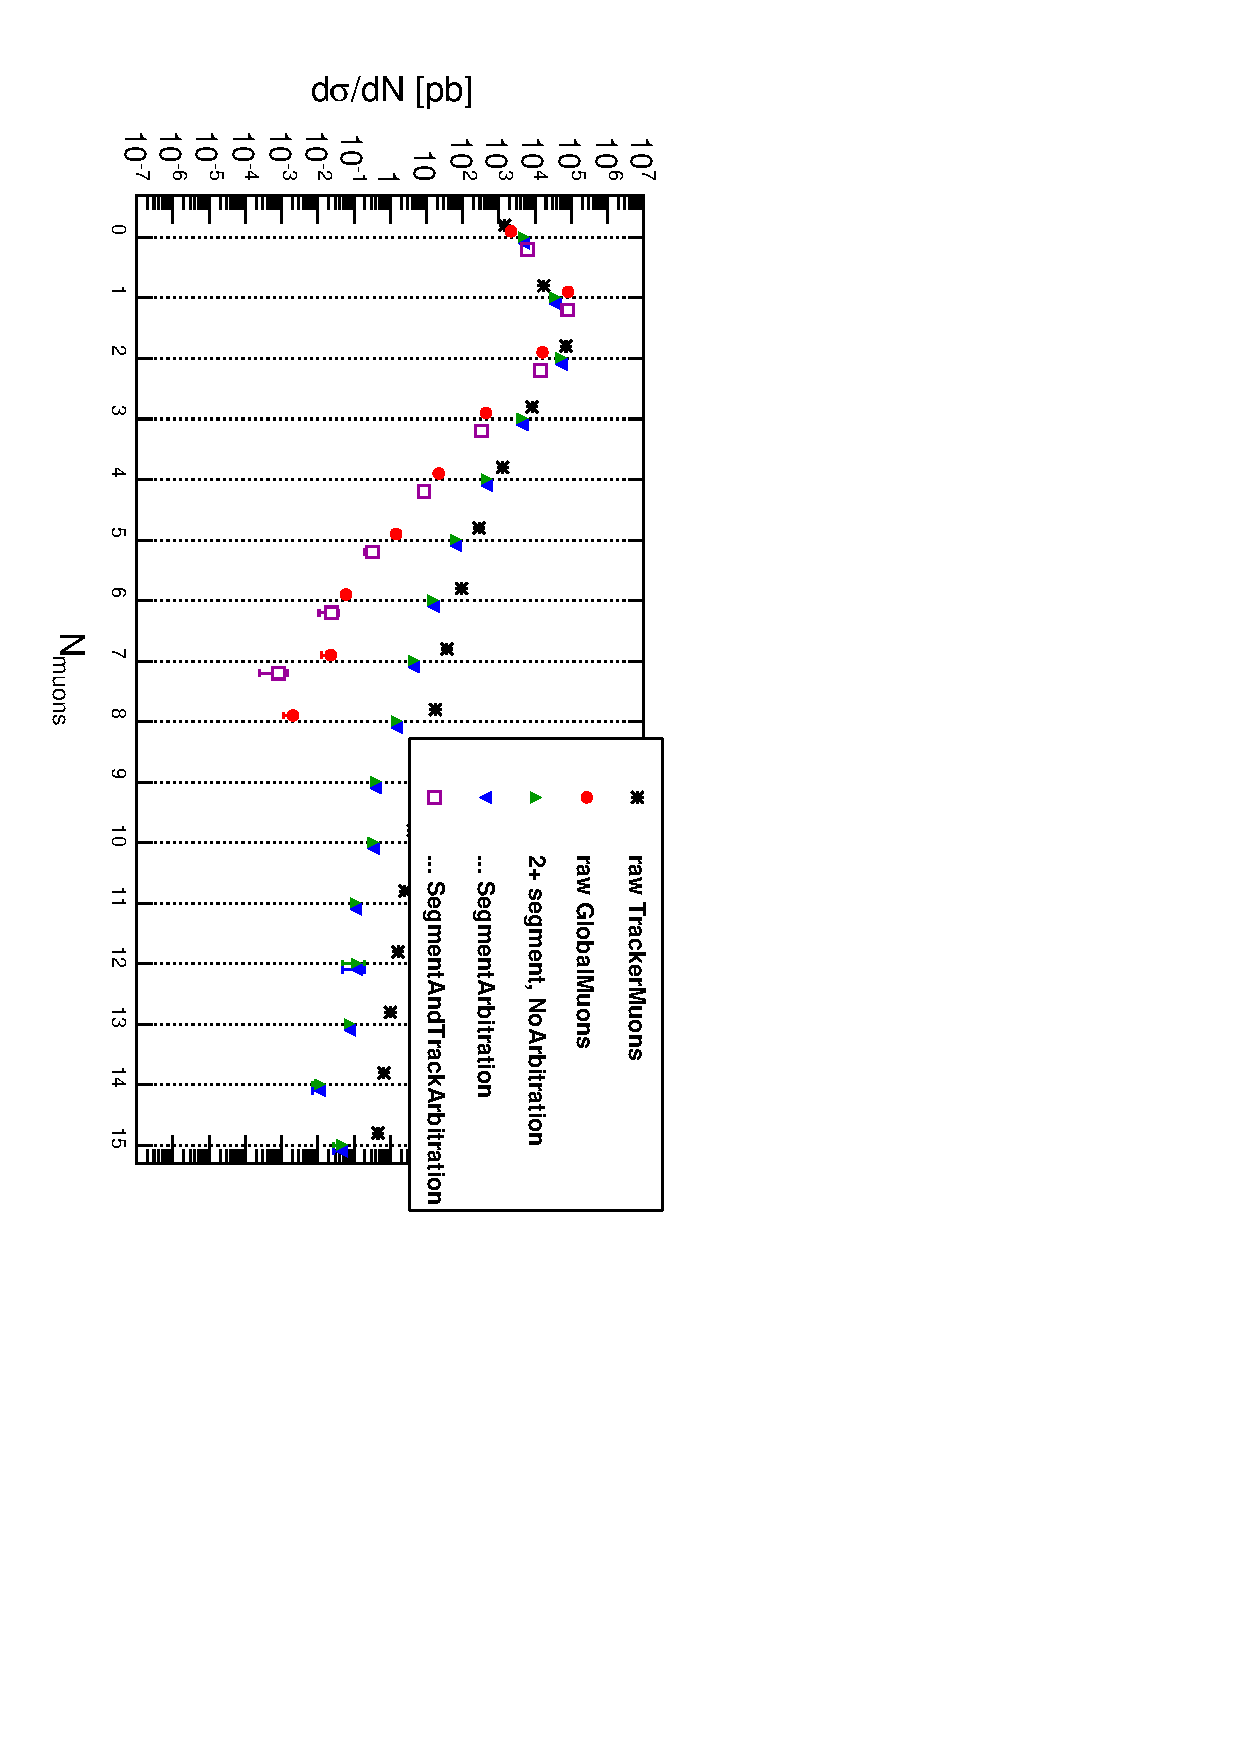
\includegraphics[height=\linewidth, angle=90]{tracks_lastpage_allreal.pdf}

\item Even with the cuts, TrackerMuons do not have inefficiencies that
  depend on closeness of muons in muon system \mbox{(right: $\mu$-pair gun efficiency as color scale vs.\ ME2 $\Delta R$, $\Delta \phi$)\hspace{-7 cm}}

\vspace{0.1 cm}
\mbox{\scriptsize (This is 3\_6\_3; GlobalMuon inefficiencies likely worse in 3\_8\_2 due to new cleaning step)\hspace{-5 cm}}
\end{itemize}
\column{0.5\linewidth}
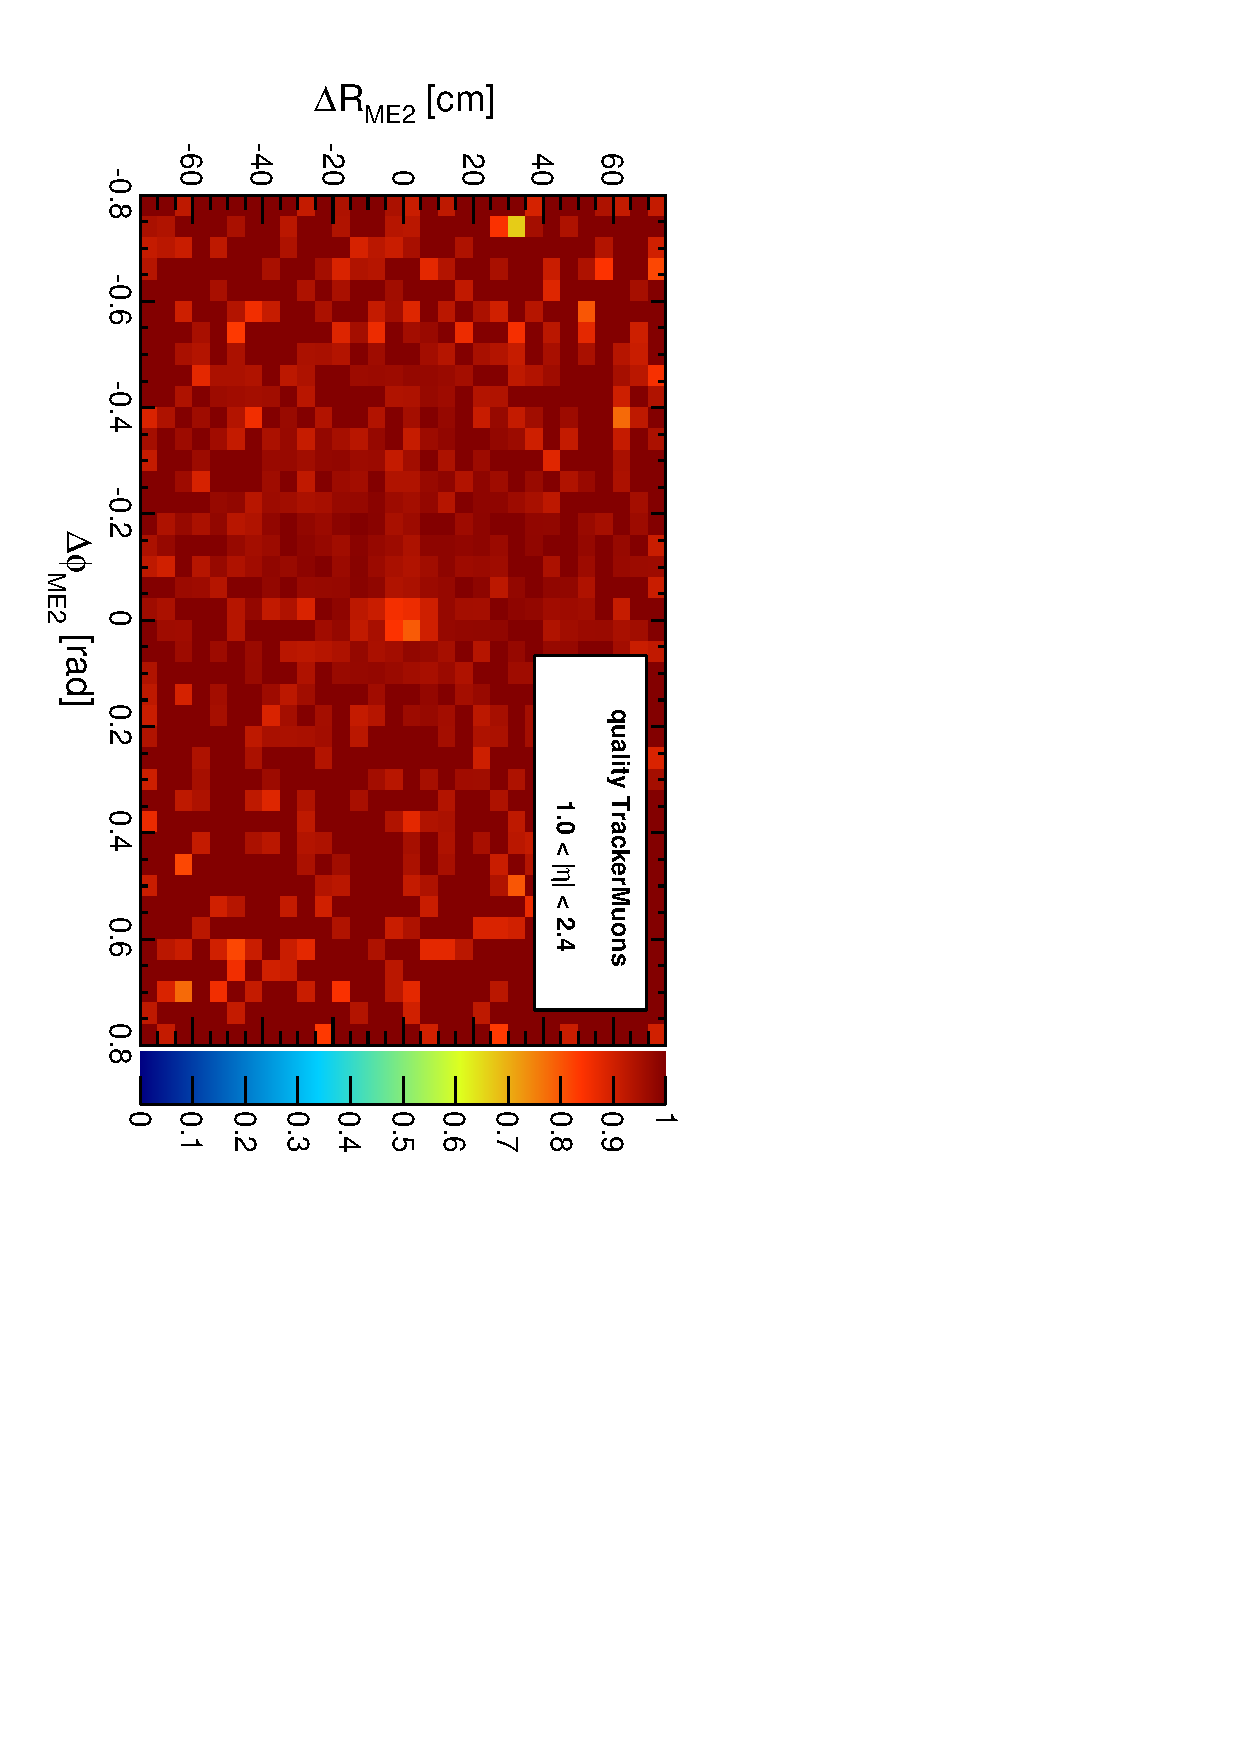
\includegraphics[height=\linewidth, angle=90]{me2_PlainTrackerMuon.pdf}

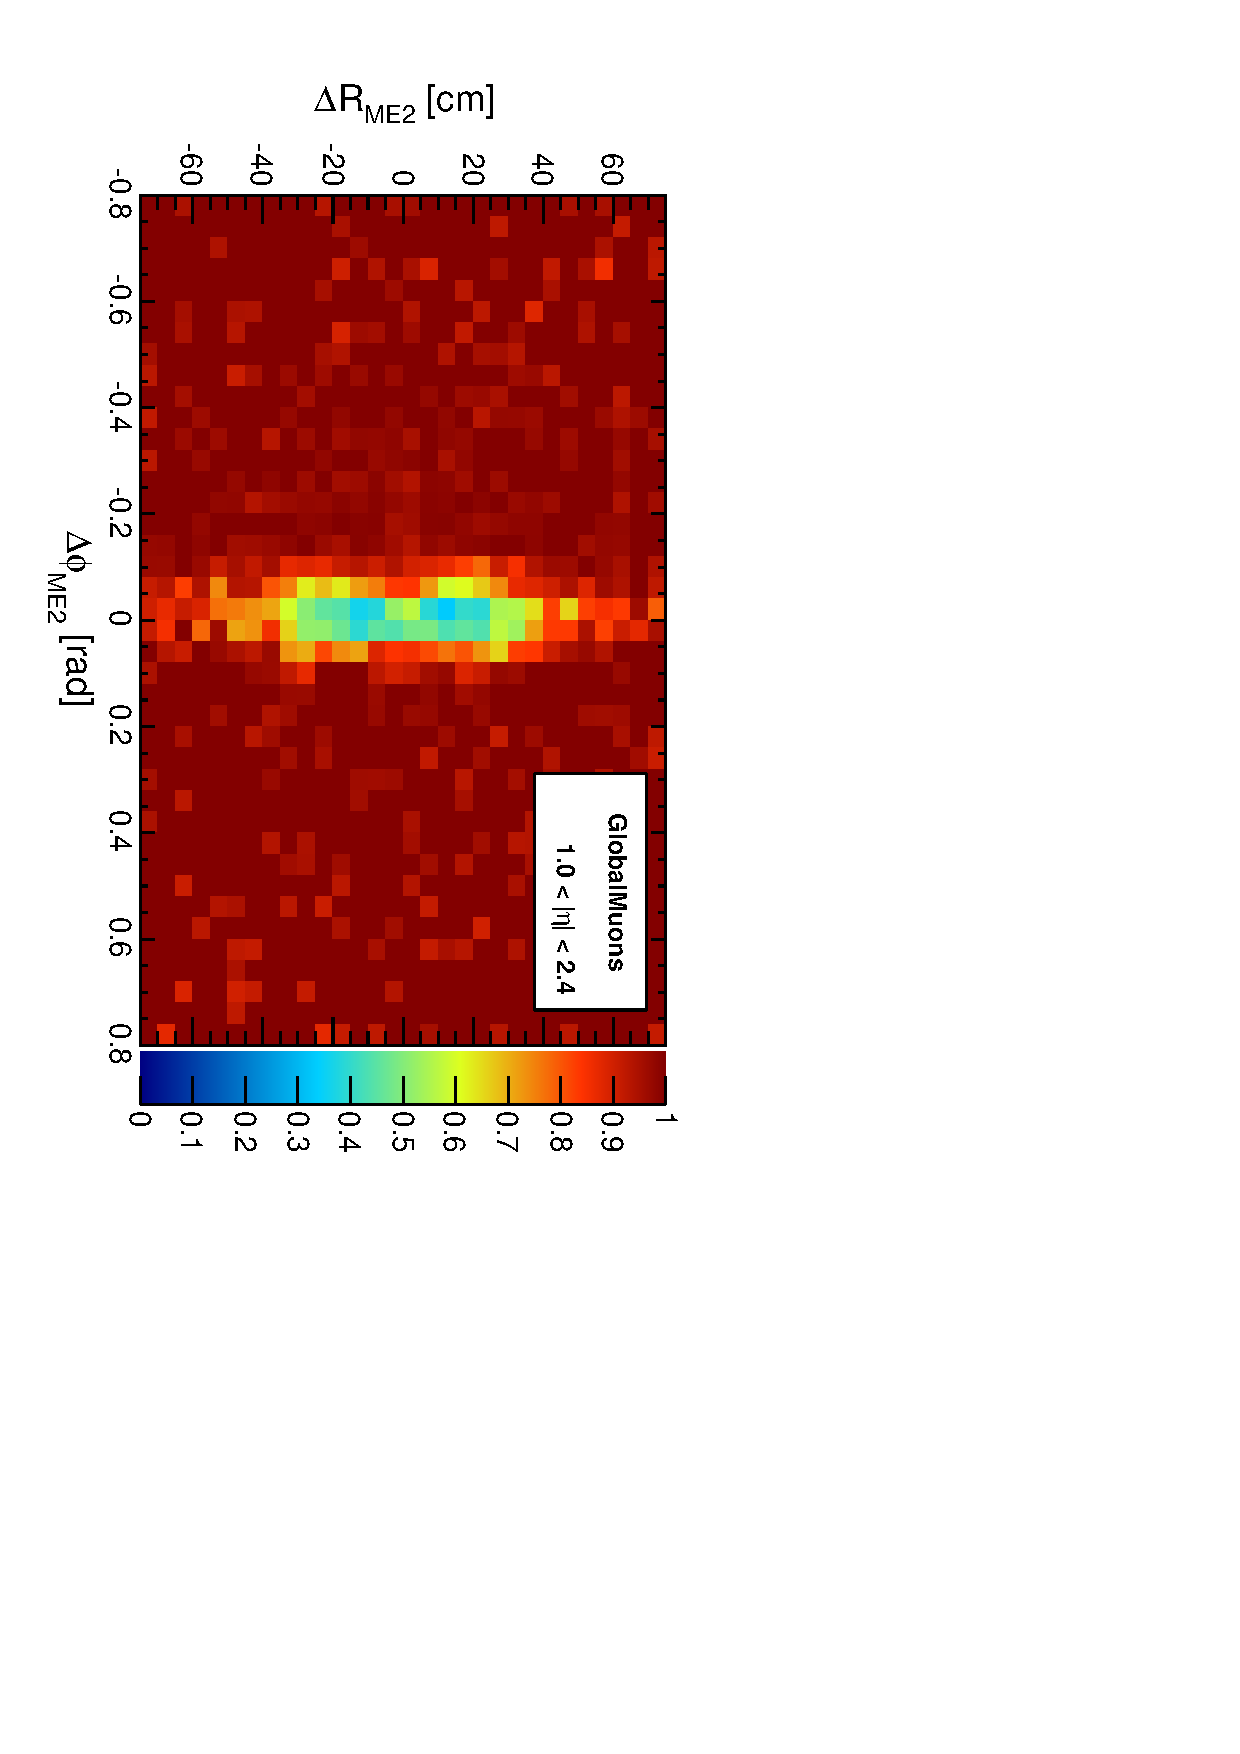
\includegraphics[height=\linewidth, angle=90]{me2_GlobalMuons.pdf}

\vspace{0.5 cm}
\end{columns}
\end{frame}

\begin{frame}
\begin{center}
\Huge \textcolor{blue}{High-level quantities in 3\_6\_3}
\end{center}
\end{frame}

\begin{frame}
\frametitle{High-level data/MC comparison}
\begin{itemize}
\item Mass distribution; data and MC independently scaled by luminosity
\item Big plot: HLT\_Mu9 with $p_T > 11$; small: HLT\_Mu5 with 7~GeV/$c$
\end{itemize}

\vspace{1.5 cm}
\hfill \only<1>{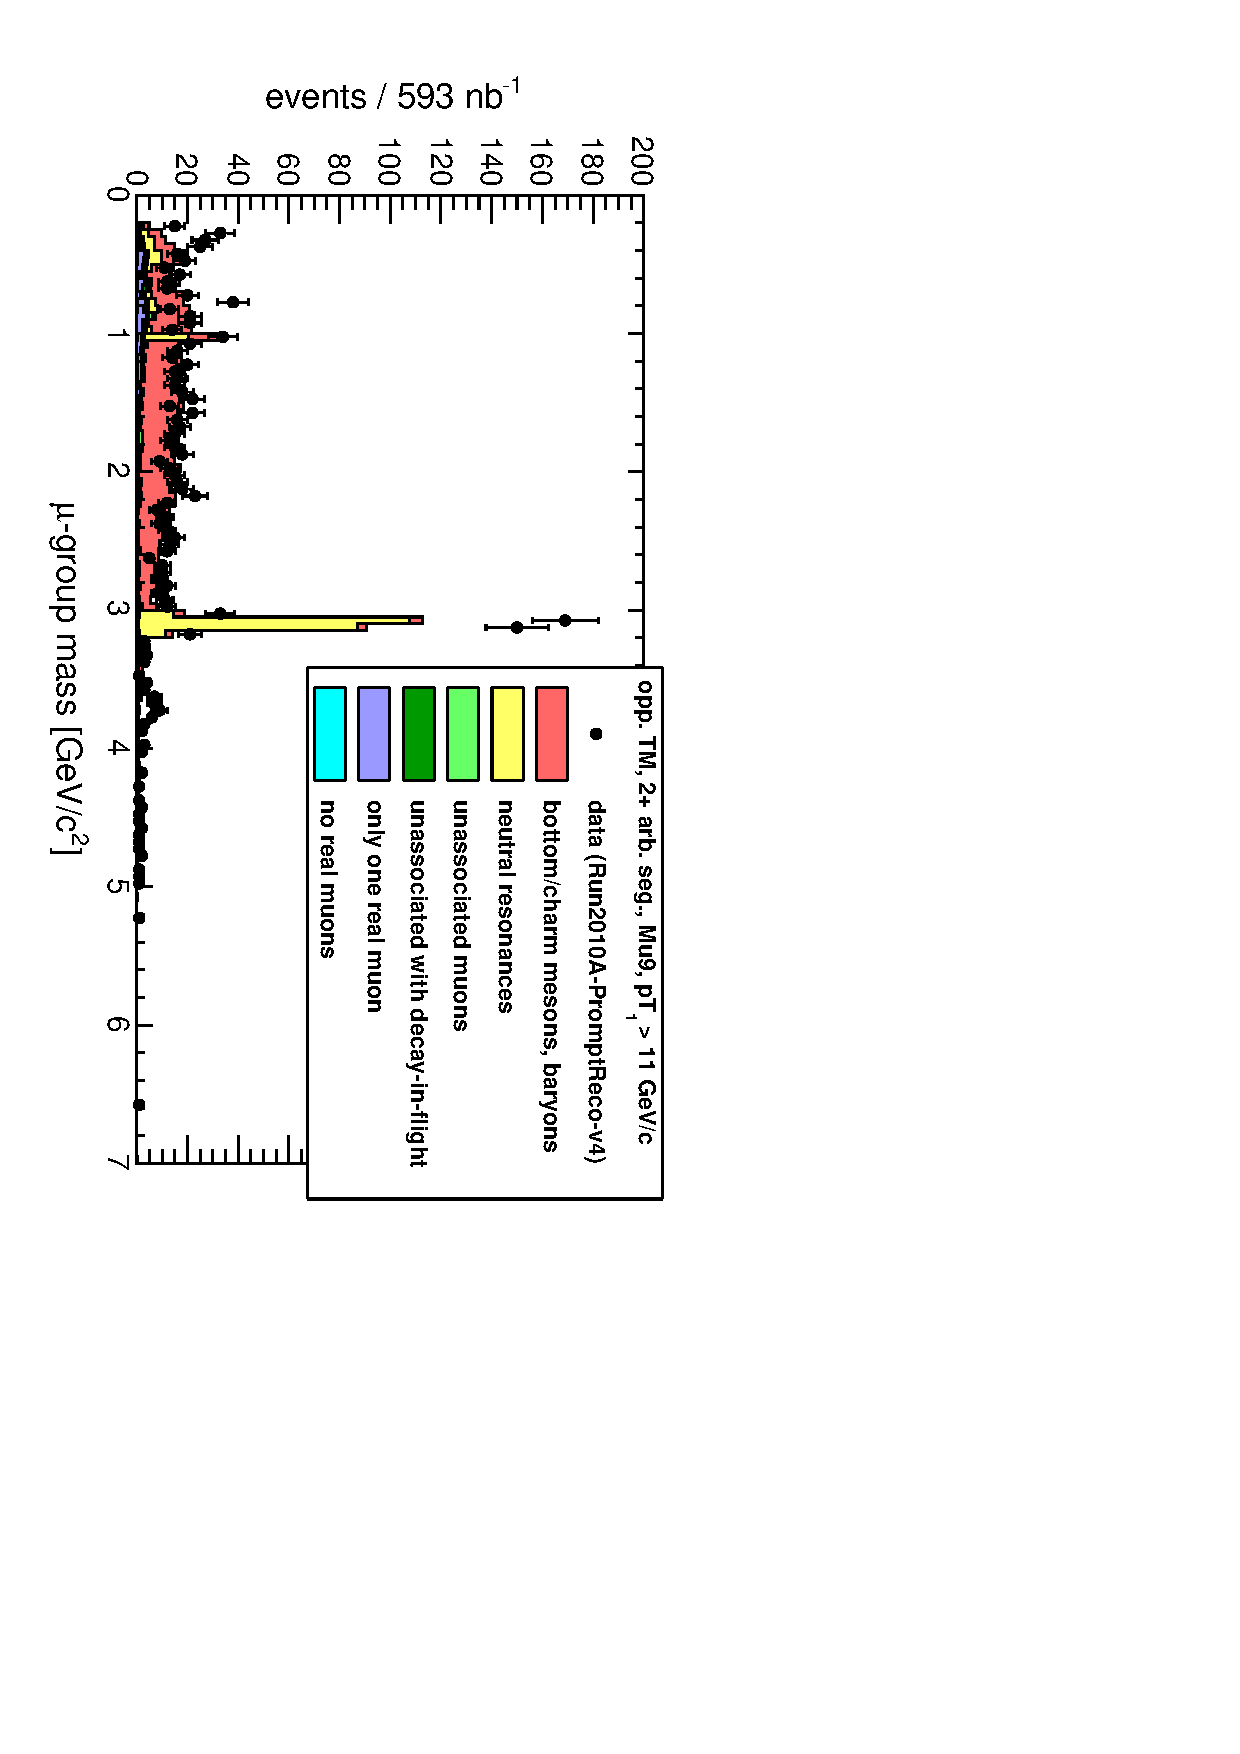
\includegraphics[height=0.9\linewidth, angle=90]{Mu9_mass_general.pdf}}\only<2>{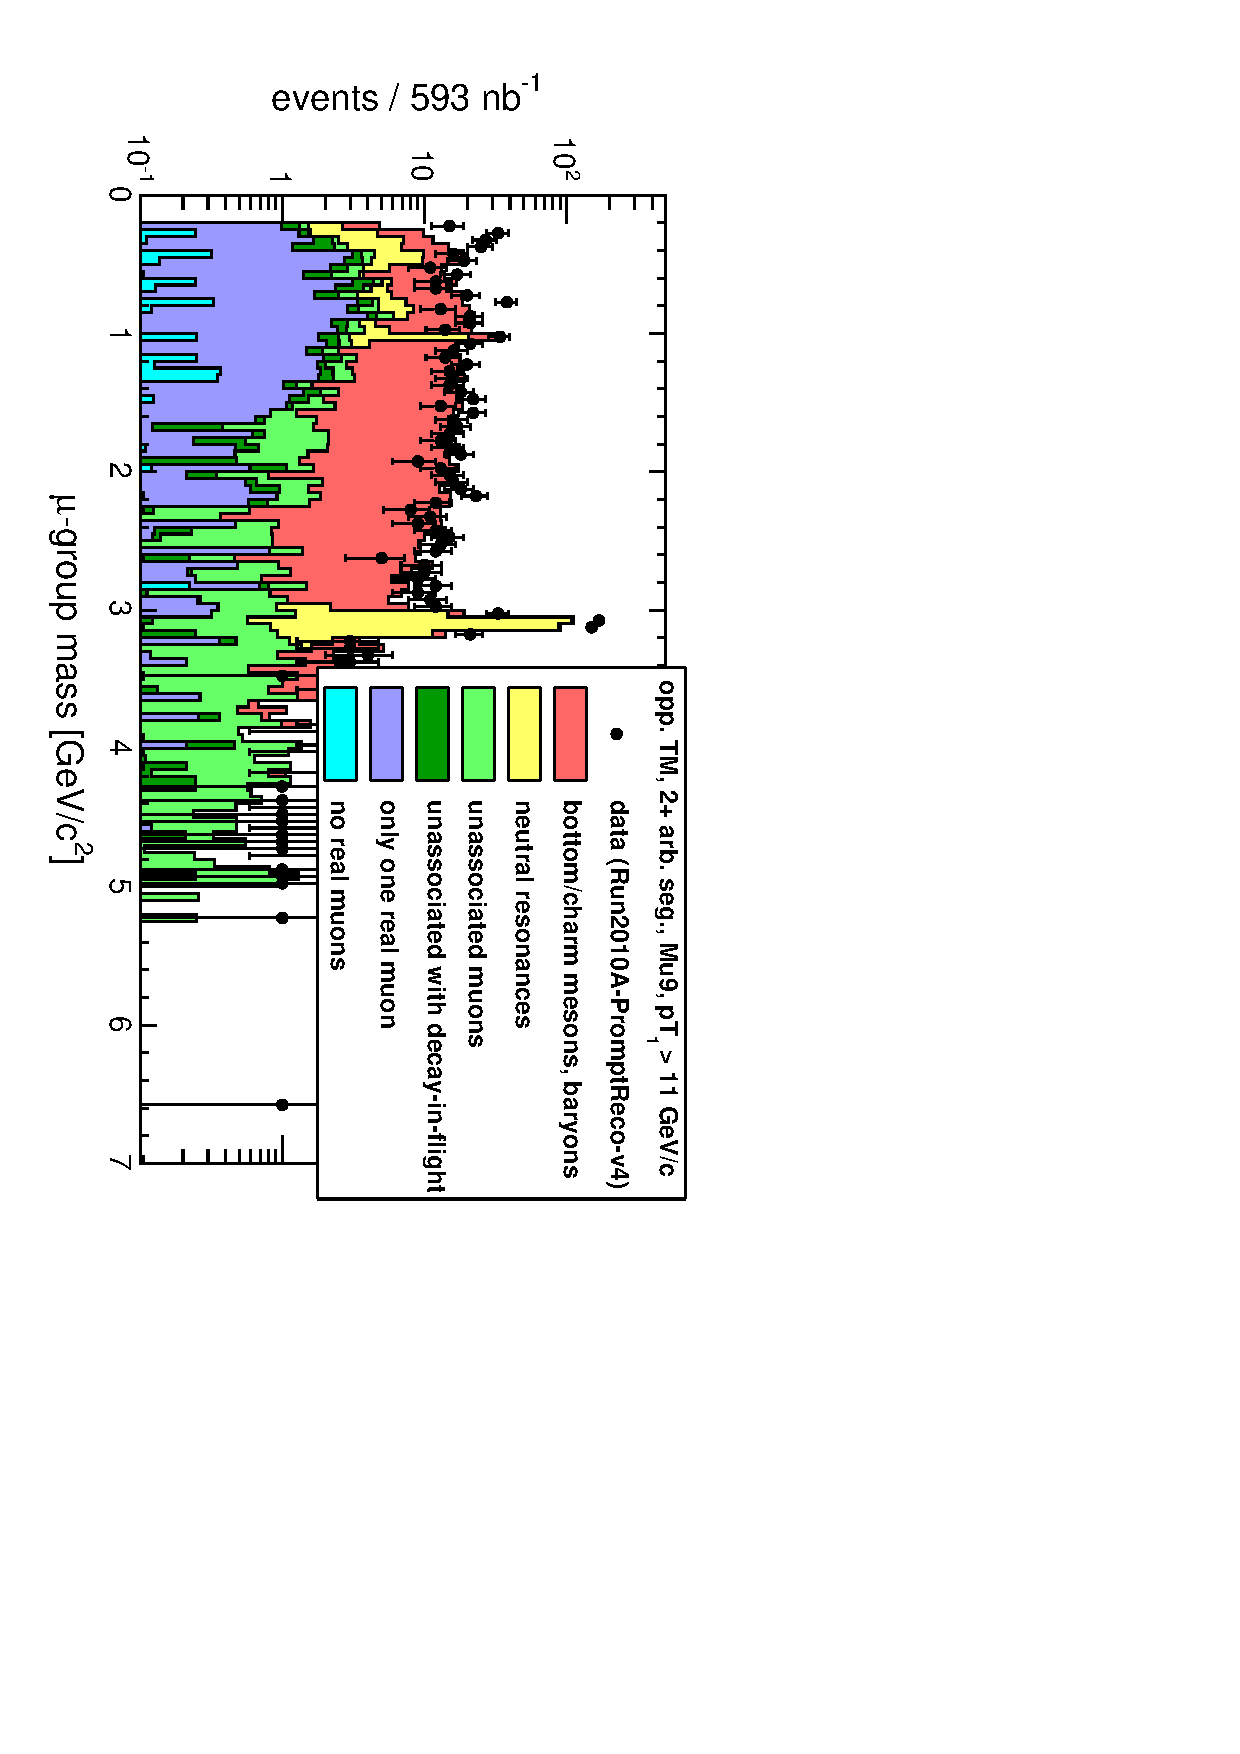
\includegraphics[height=0.9\linewidth, angle=90]{Mu9_mass_general_log.pdf}}

\vspace{-6.7 cm}
\begin{columns}
\column{0.45\linewidth}
\only<1>{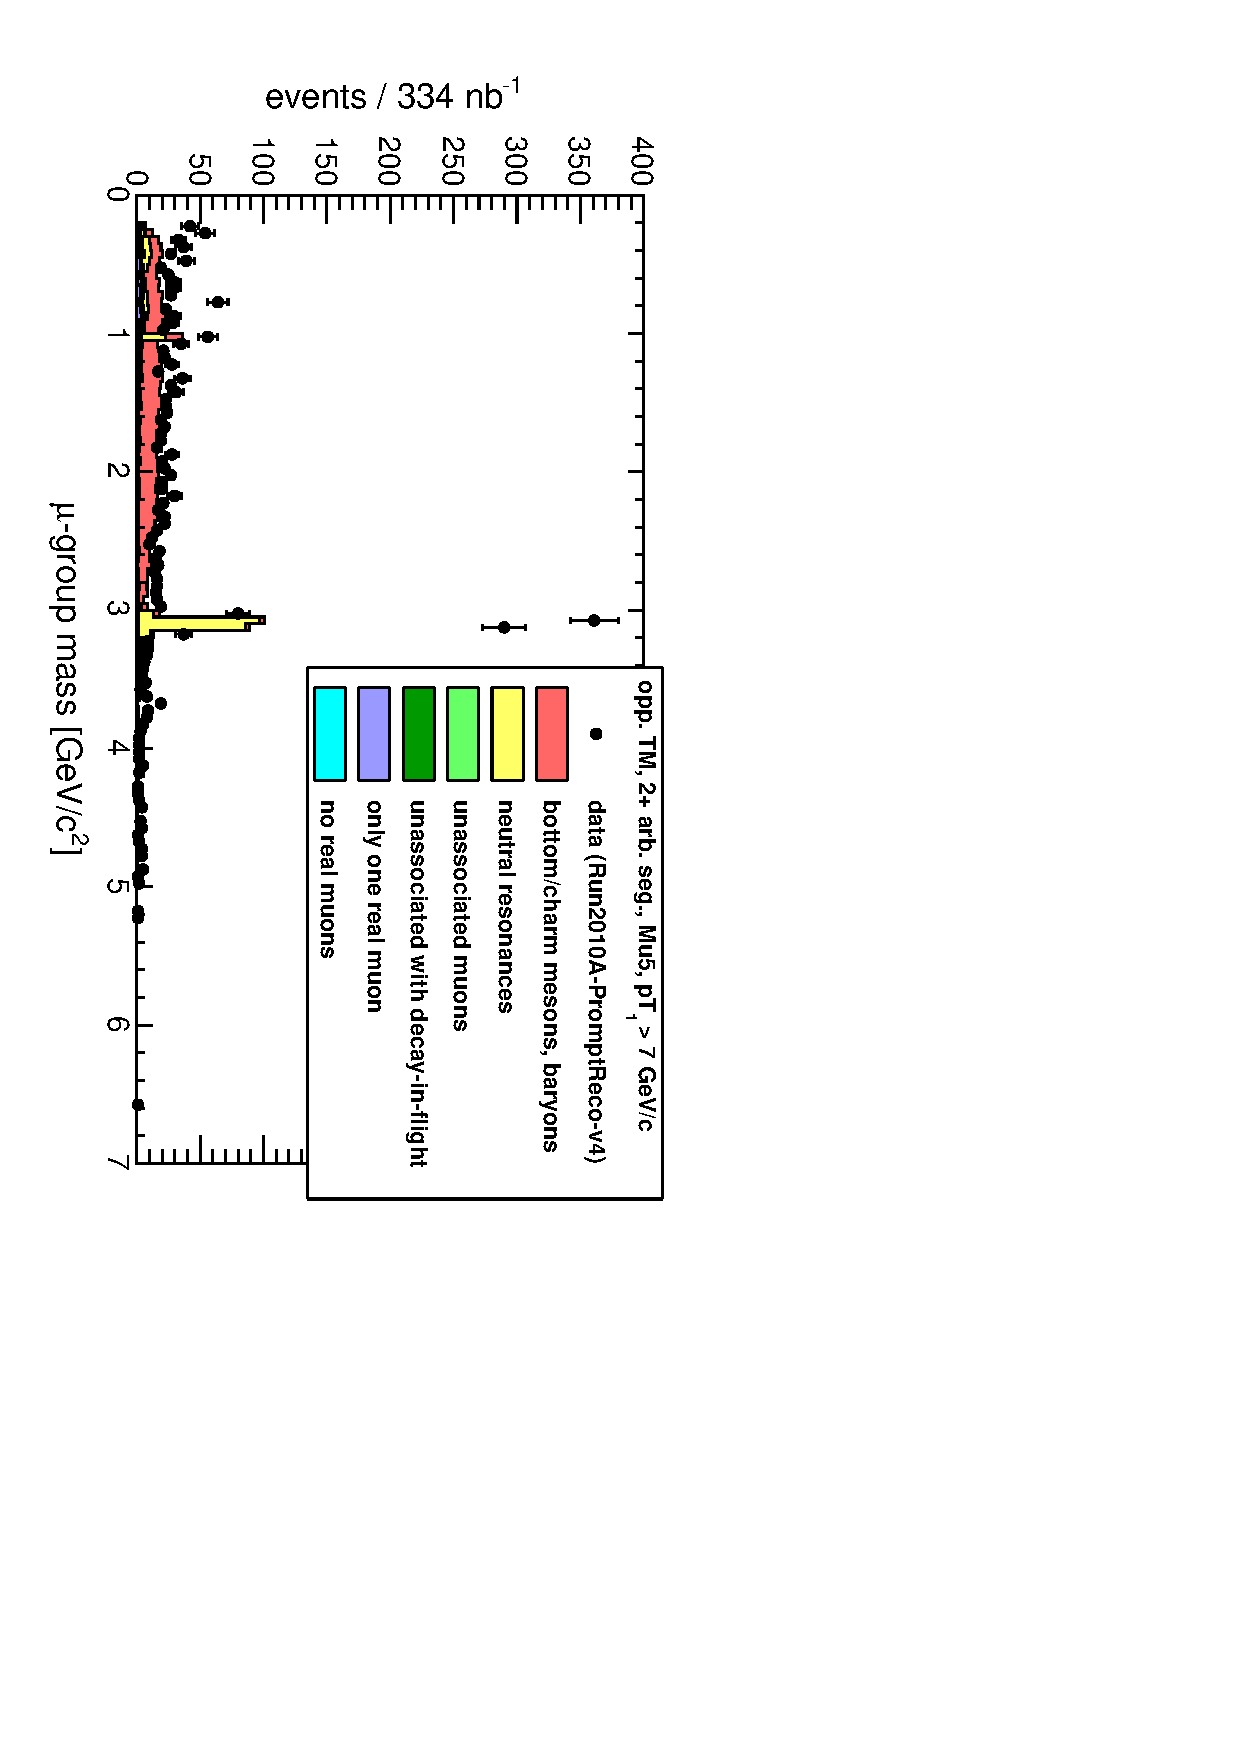
\includegraphics[height=\linewidth, angle=90]{Mu5_mass_general.pdf}}\only<2>{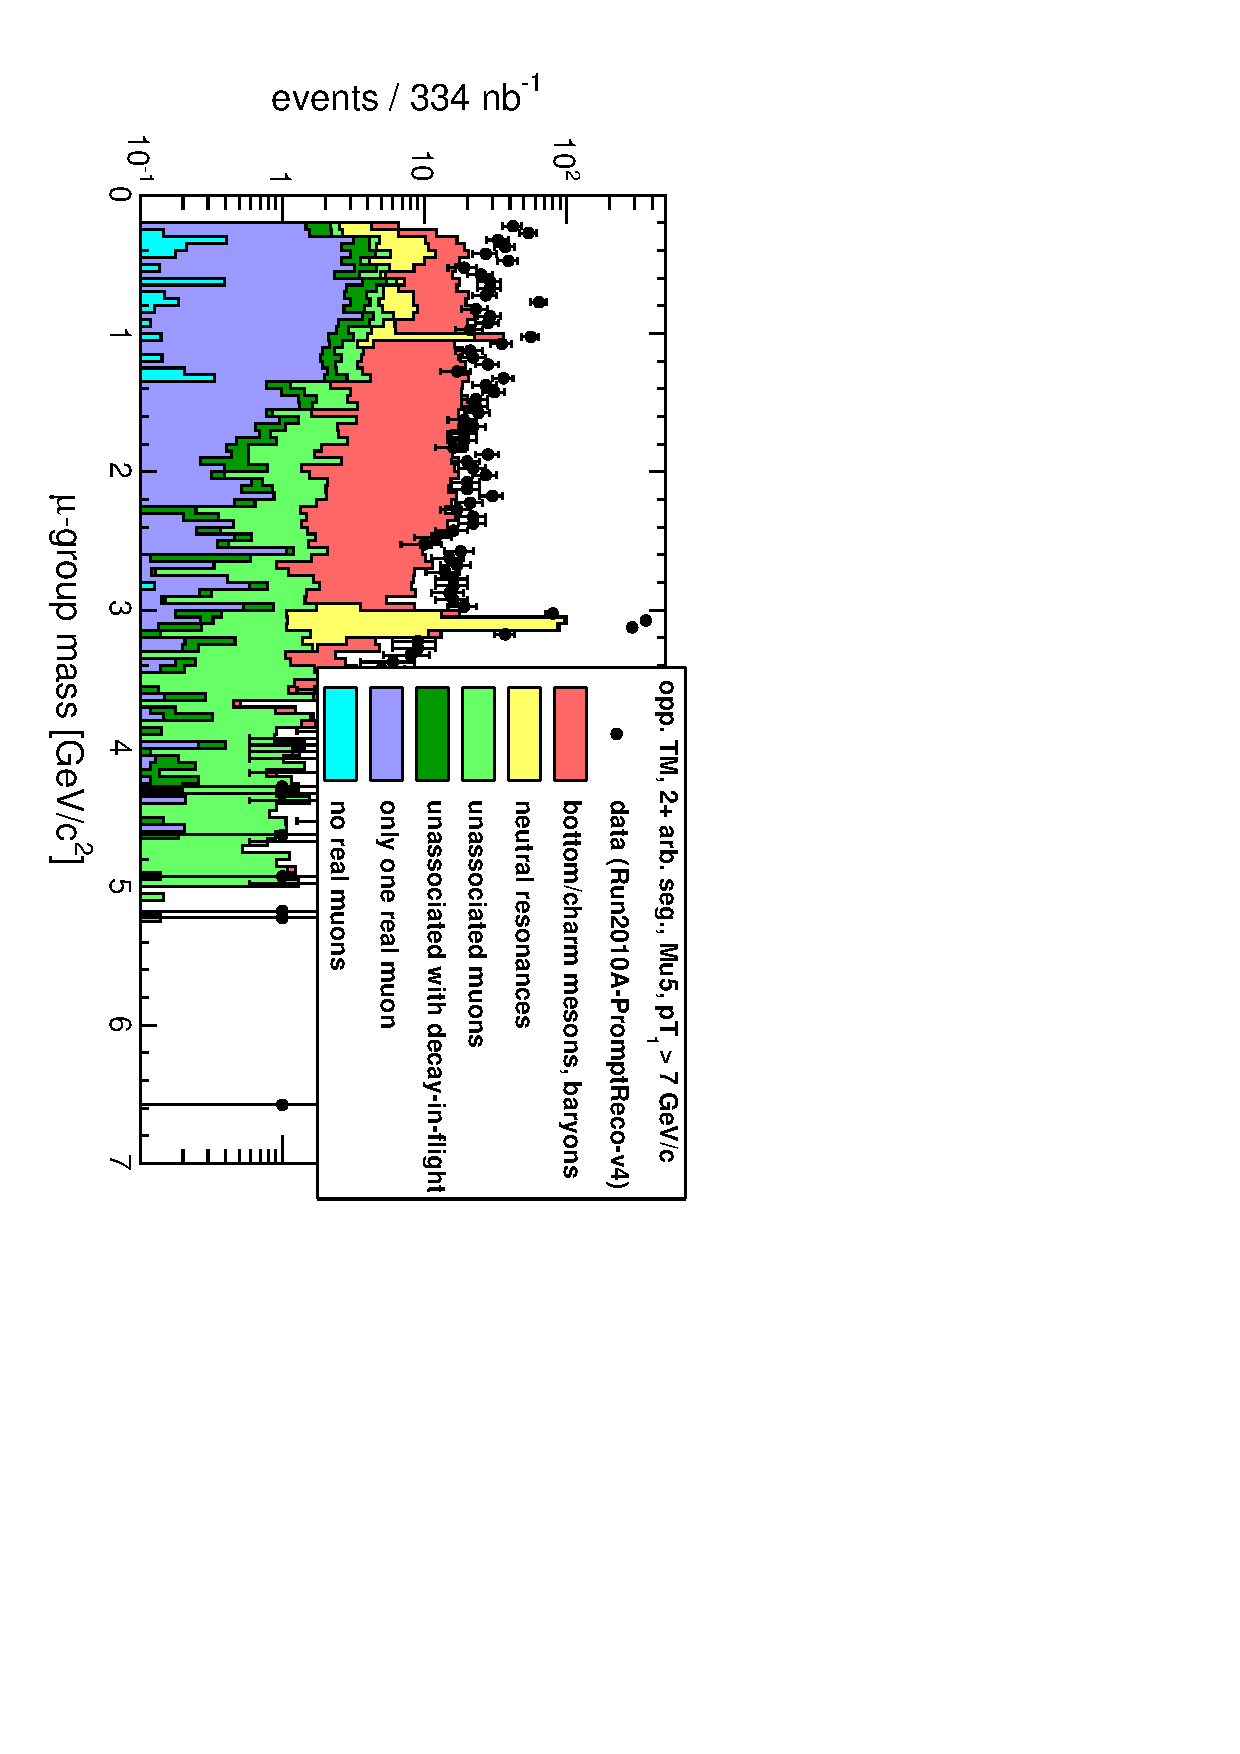
\includegraphics[height=\linewidth, angle=90]{Mu5_mass_general_log.pdf}}
\column{0.54\linewidth}
\vspace{-2 cm}
\begin{itemize}
\item Trigger simulation not applied \\ to Monte Carlo
\end{itemize}
\end{columns}

\vspace{6 cm}
\end{frame}

\begin{frame}
\frametitle{High-level data/MC comparison}
\begin{itemize}
\item Prompt $J/\psi$ (and $\psi'$) are not in InclusiveMu5\_Pt*
\item $p_T$ of $\mu$-groups with masses near $J/\psi$ peak shows that the missing \\ \hspace{5.15 cm} events are at low momentum
\end{itemize}

\vspace{-0.3 cm}
\vspace{1.5 cm}
\hfill 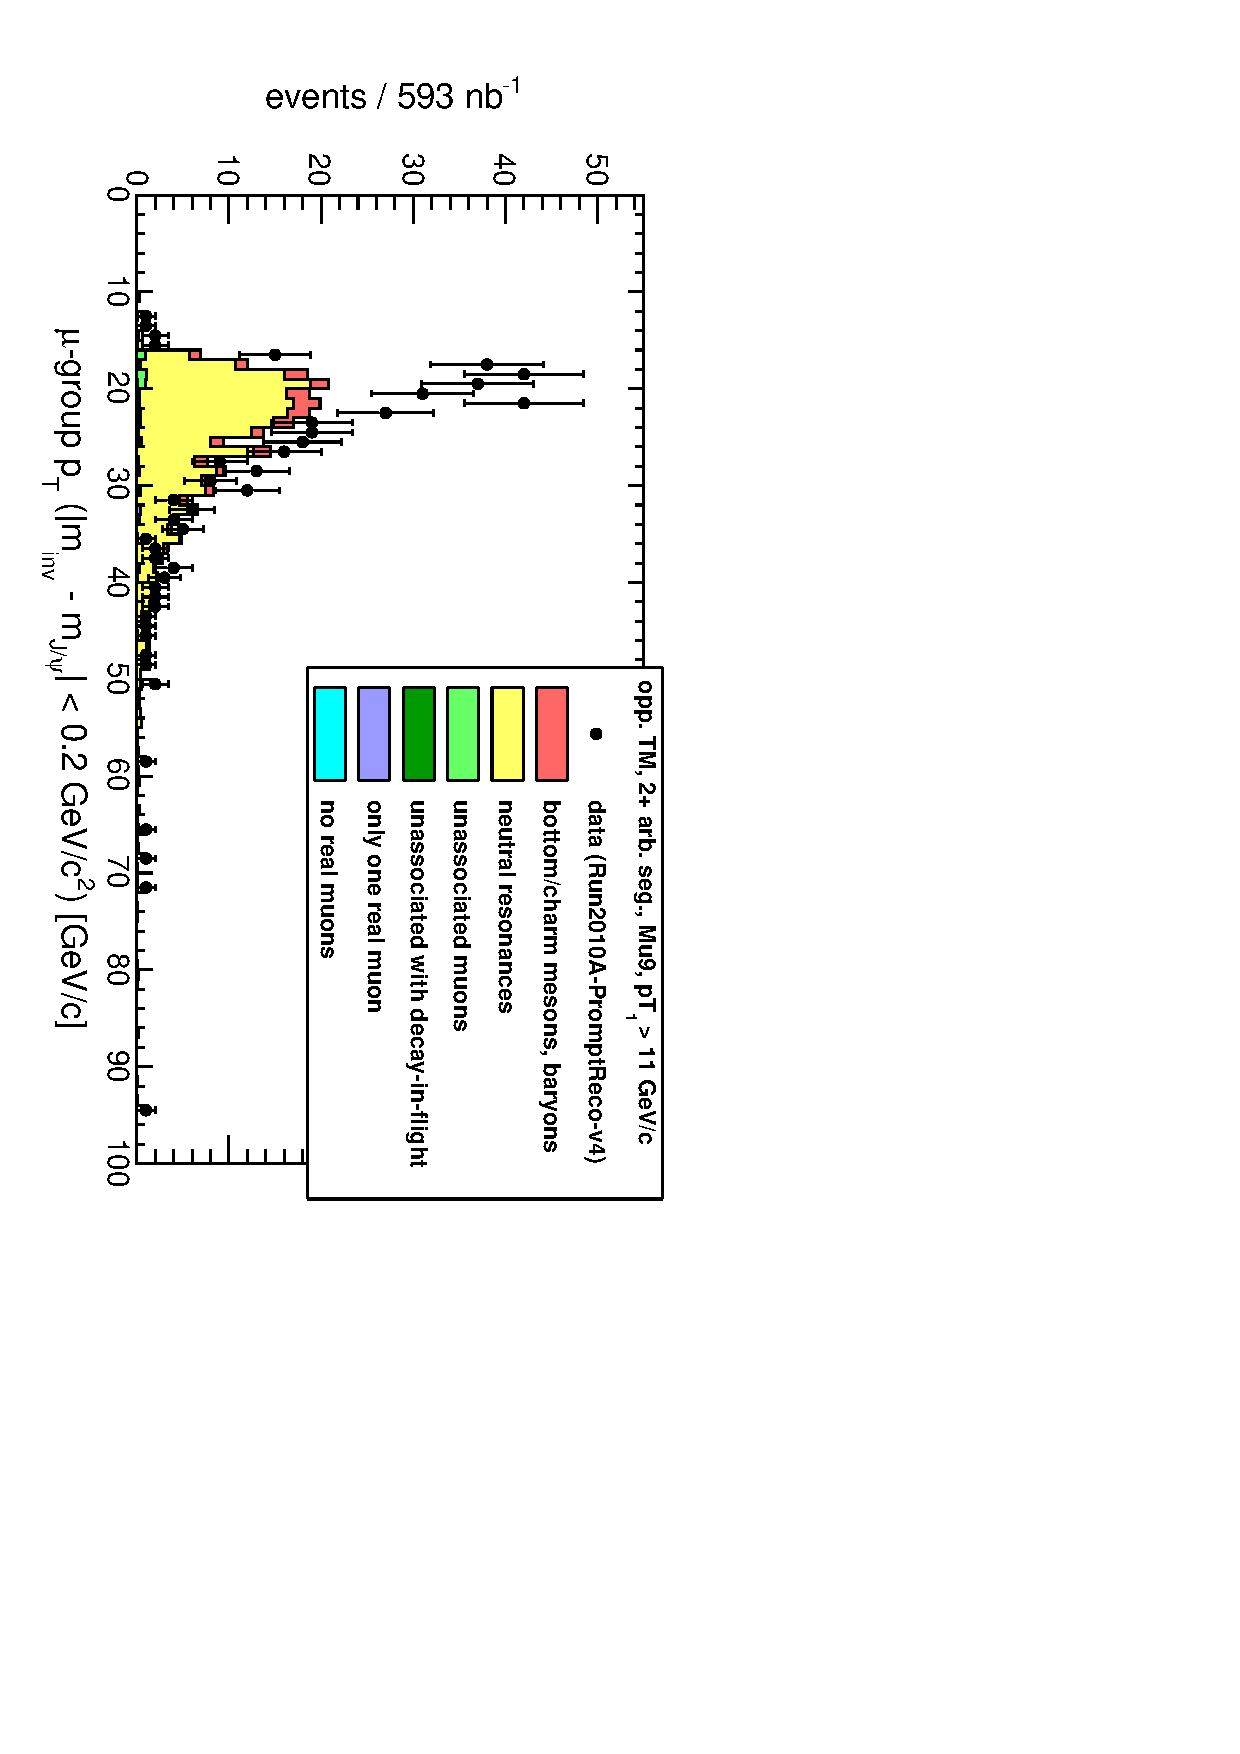
\includegraphics[height=0.9\linewidth, angle=90]{Mu9_pt_jpsi.pdf}

\vspace{-6.7 cm}
\begin{columns}
\column{0.45\linewidth}
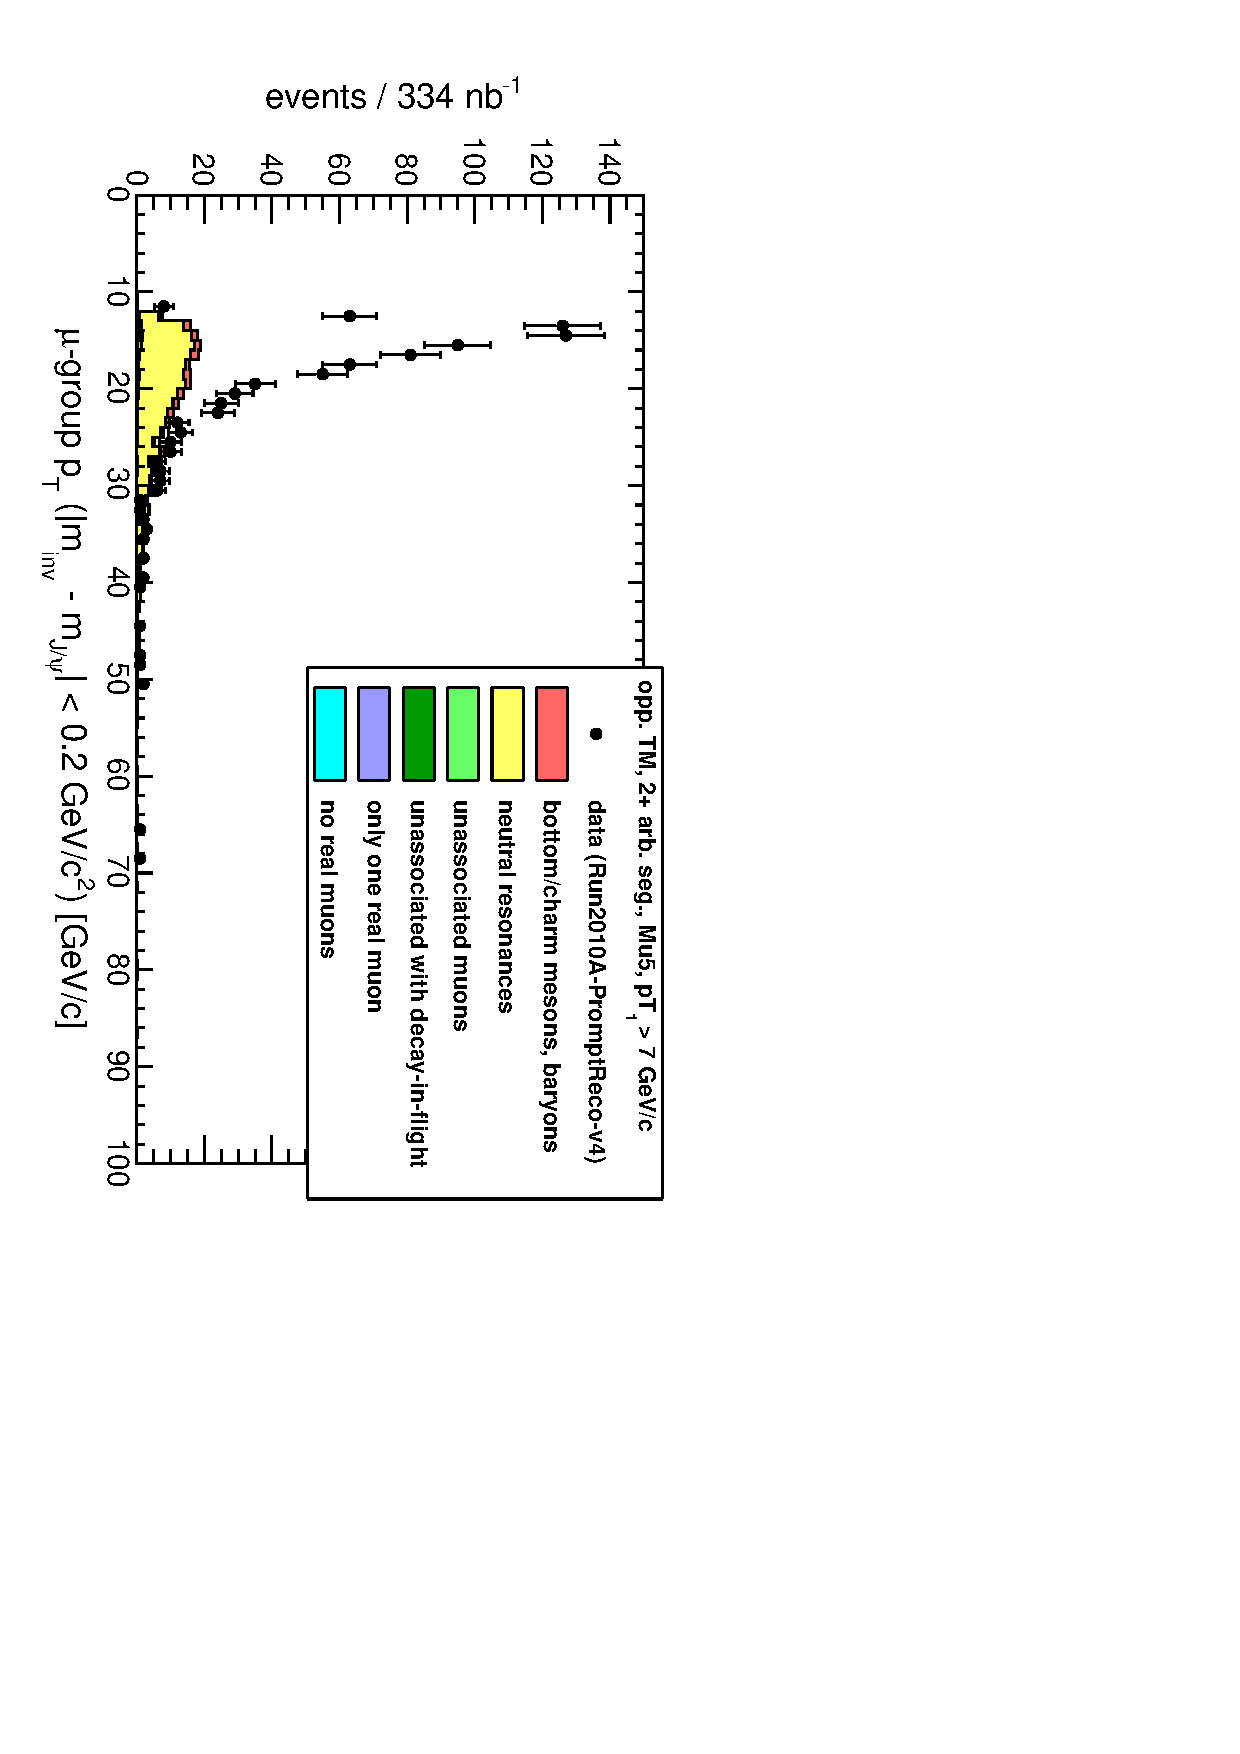
\includegraphics[height=\linewidth, angle=90]{Mu5_pt_jpsi.pdf}
\column{0.54\linewidth}
\vspace{0.3 cm}
\vspace{-2 cm}
\begin{itemize}
\item Prompt $J/\psi$ and $\psi'$ will be included in future 3\_8\_2 study
\end{itemize}
\end{columns}

\vspace{6 cm}
\end{frame}

\begin{frame}
\frametitle{High-level data/MC comparison}
\begin{columns}
\column{0.45\linewidth}
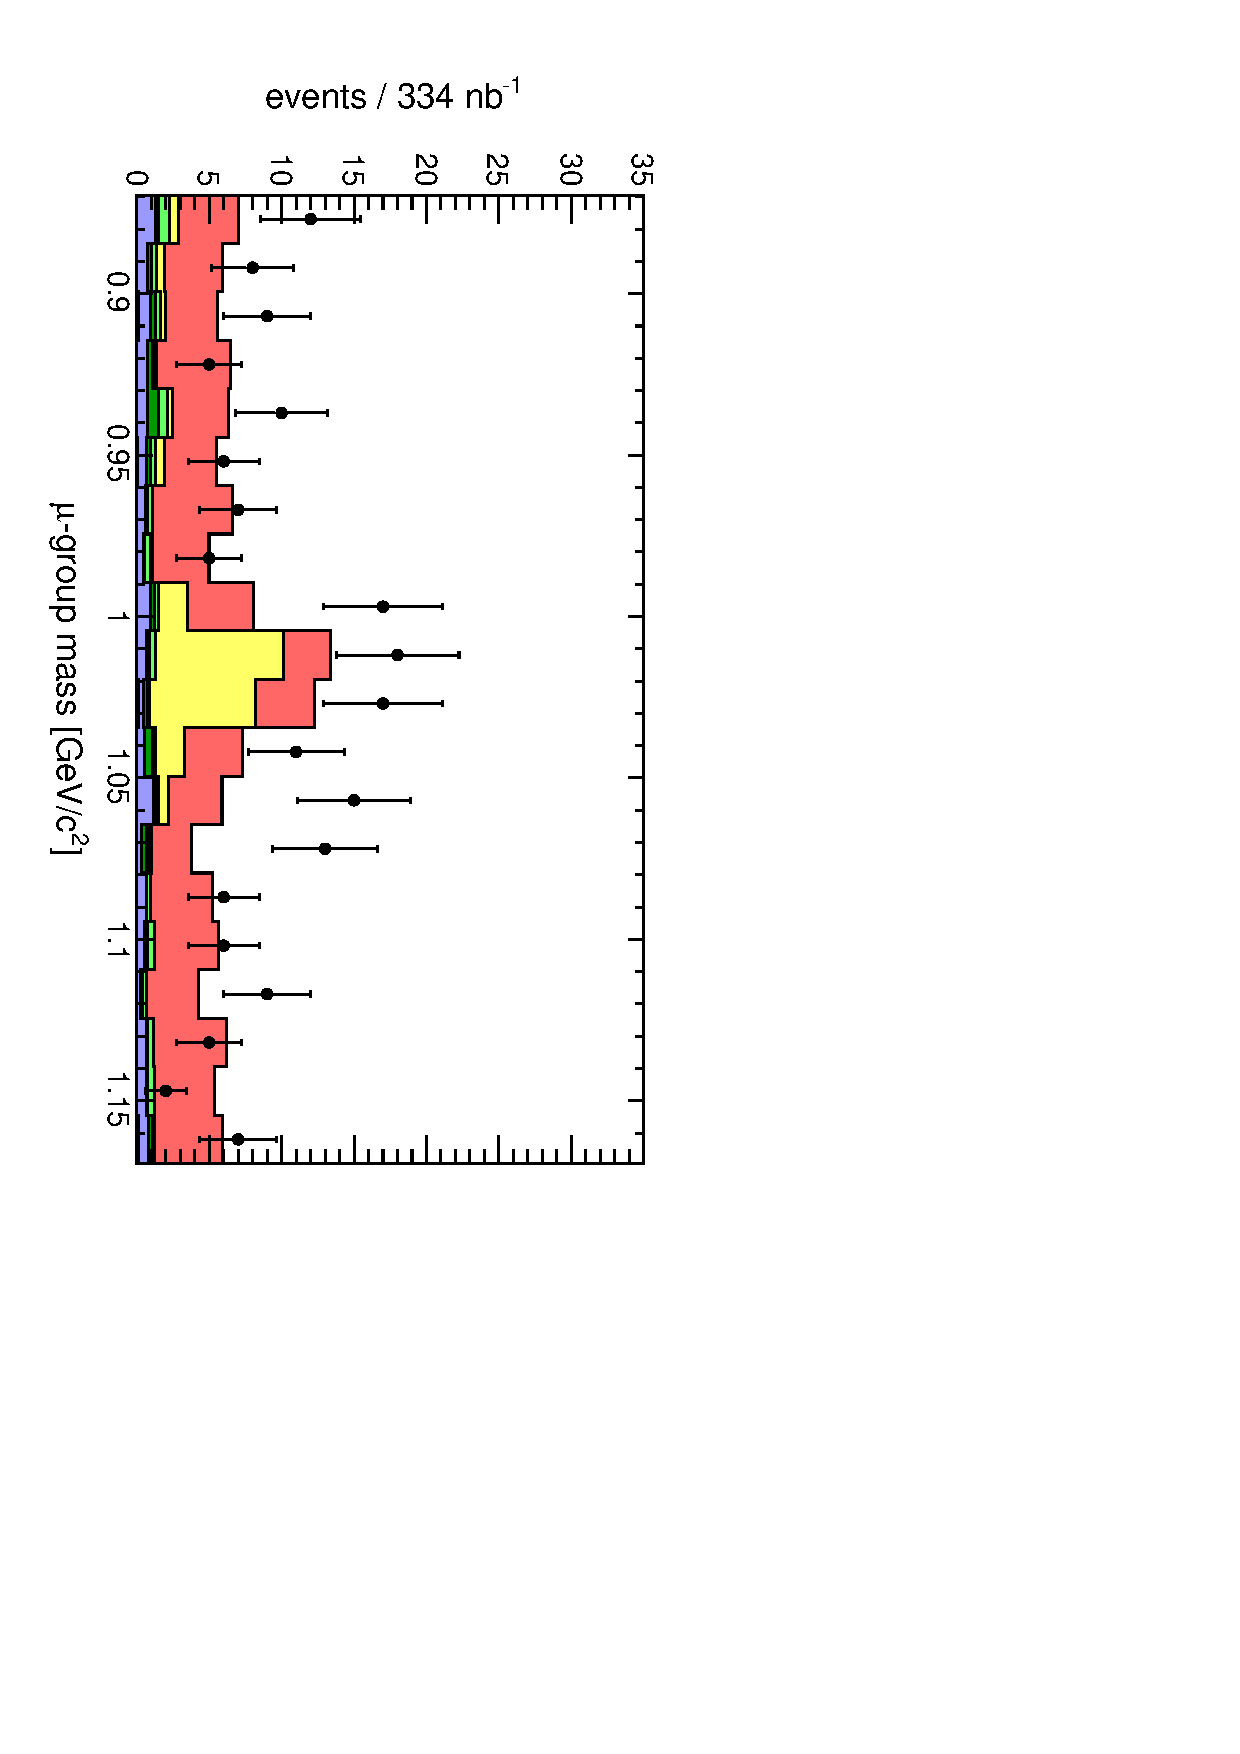
\includegraphics[height=\linewidth, angle=90]{Mu5_mass_phi.pdf}

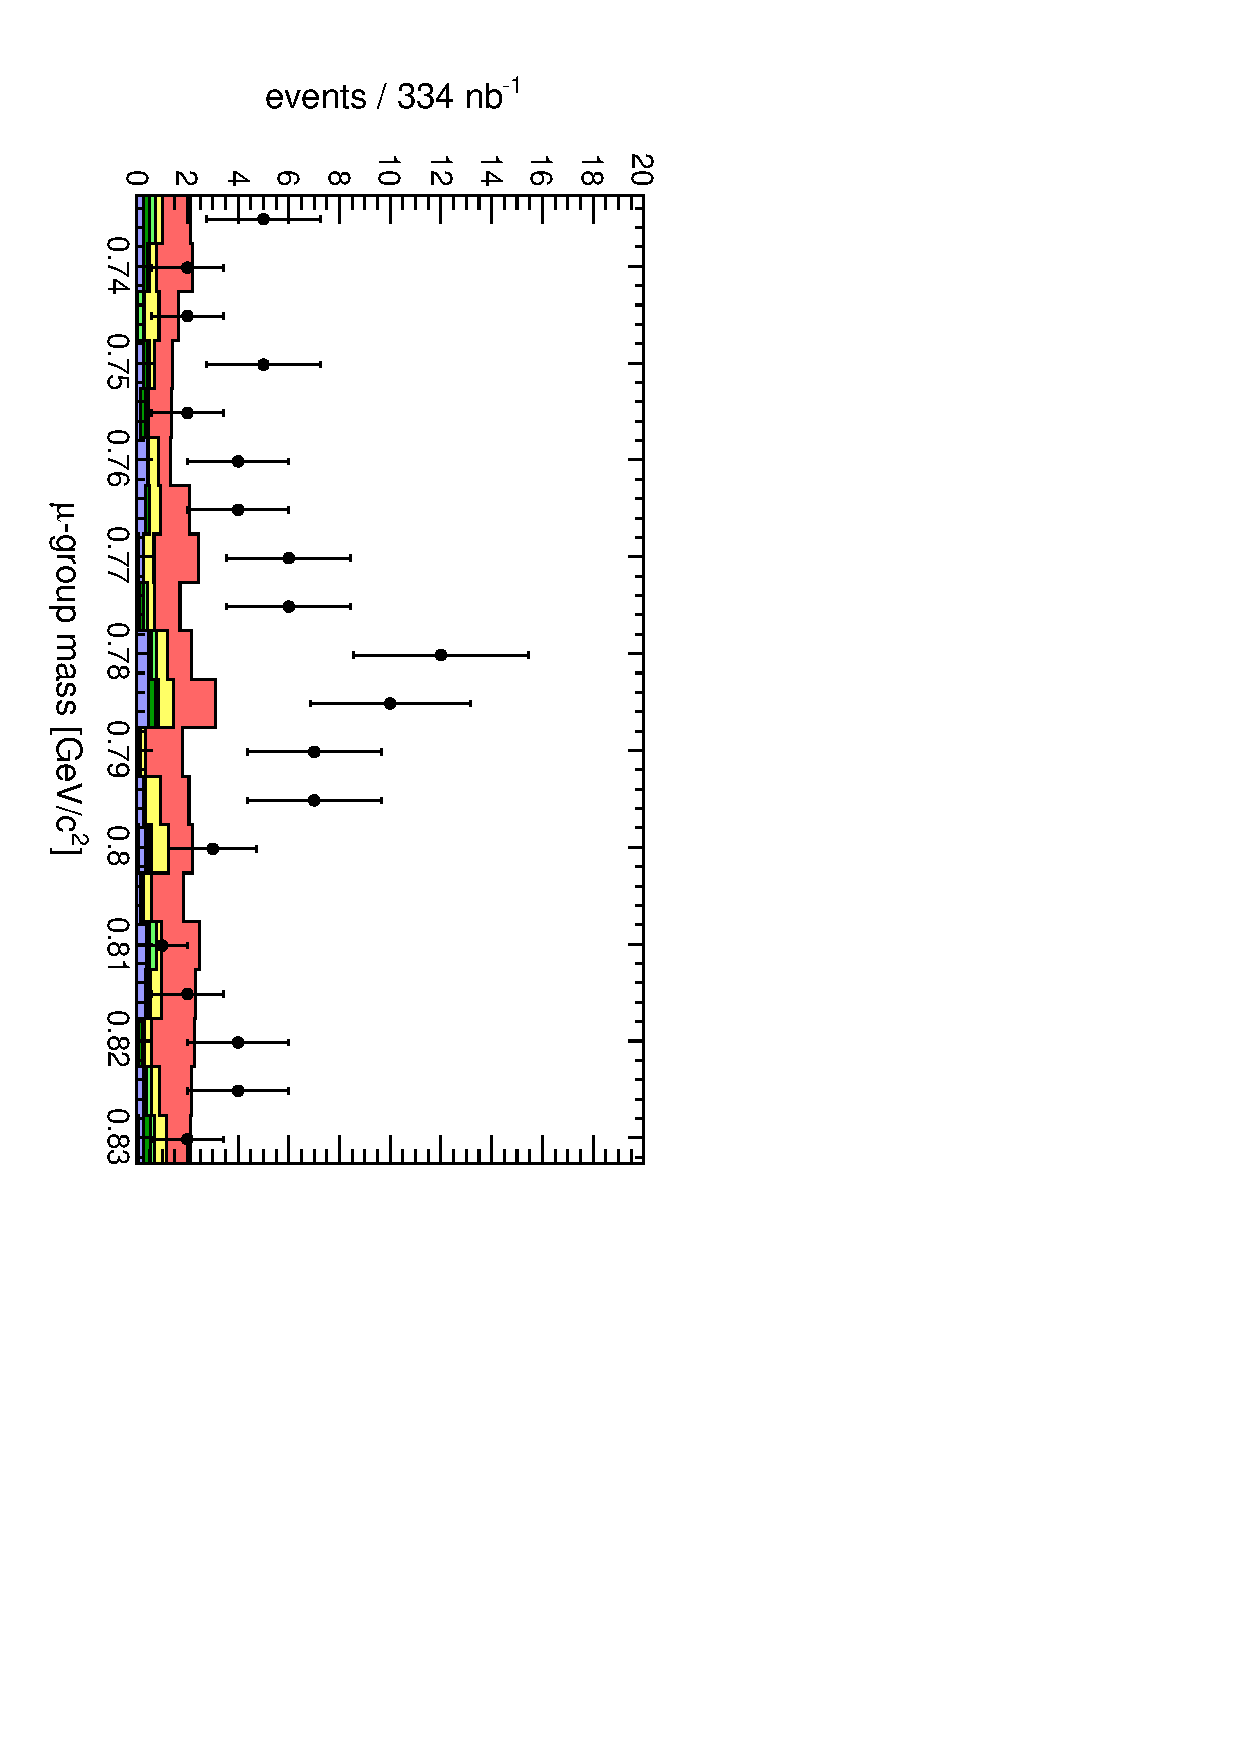
\includegraphics[height=\linewidth, angle=90]{Mu5_mass_omg.pdf}

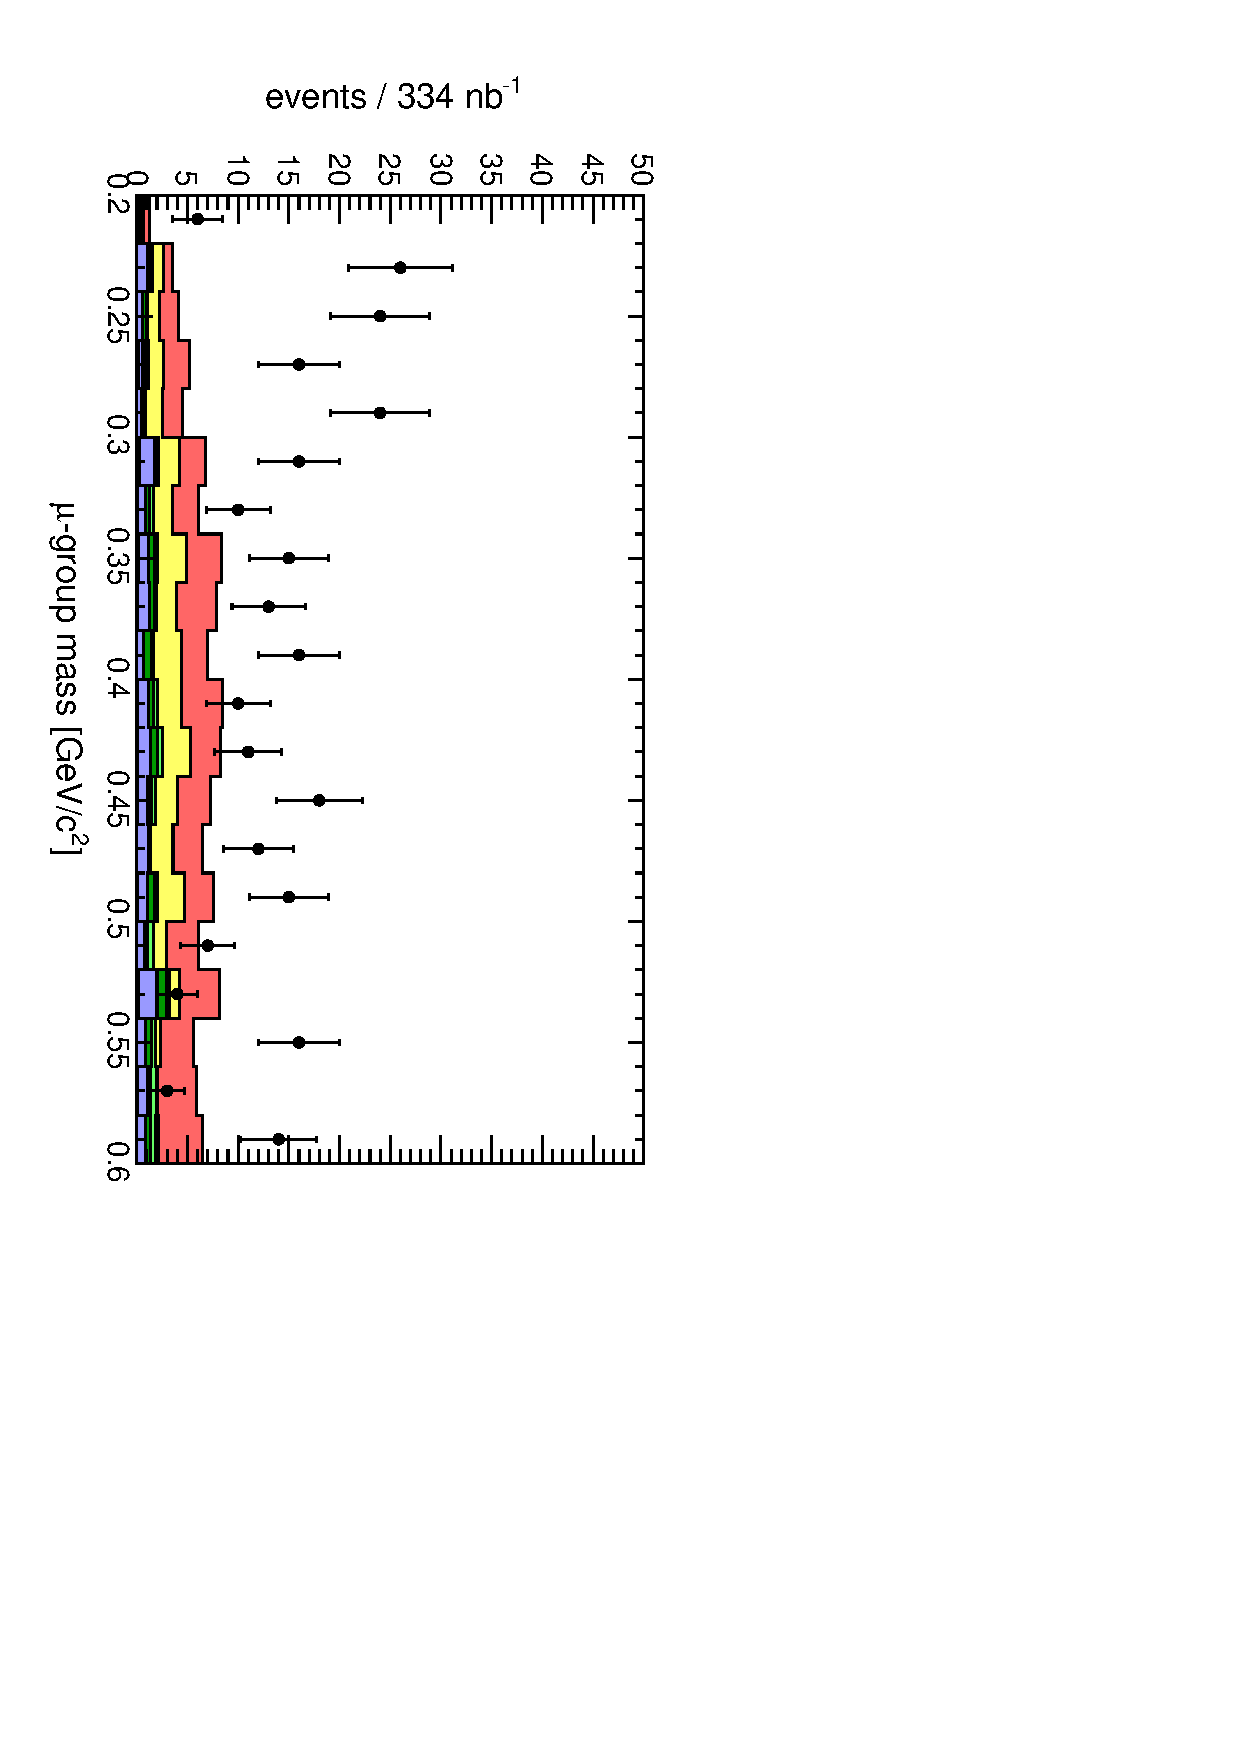
\includegraphics[height=\linewidth, angle=90]{Mu5_mass_eta.pdf}

\column{0.54\linewidth}
\begin{itemize}
\item Zoom in with HLT\_Mu5 sample to see more low-mass resonances

\item $\phi(1020) \to \mu\mu$ is visible in data/MC but underproduced?

\item $\omega(782)$ is in data but not MC

\item $\eta(548) \to \mu\mu(\gamma)$ is not responsible for the excess at low mass
\end{itemize}

\vspace{0.75 cm}
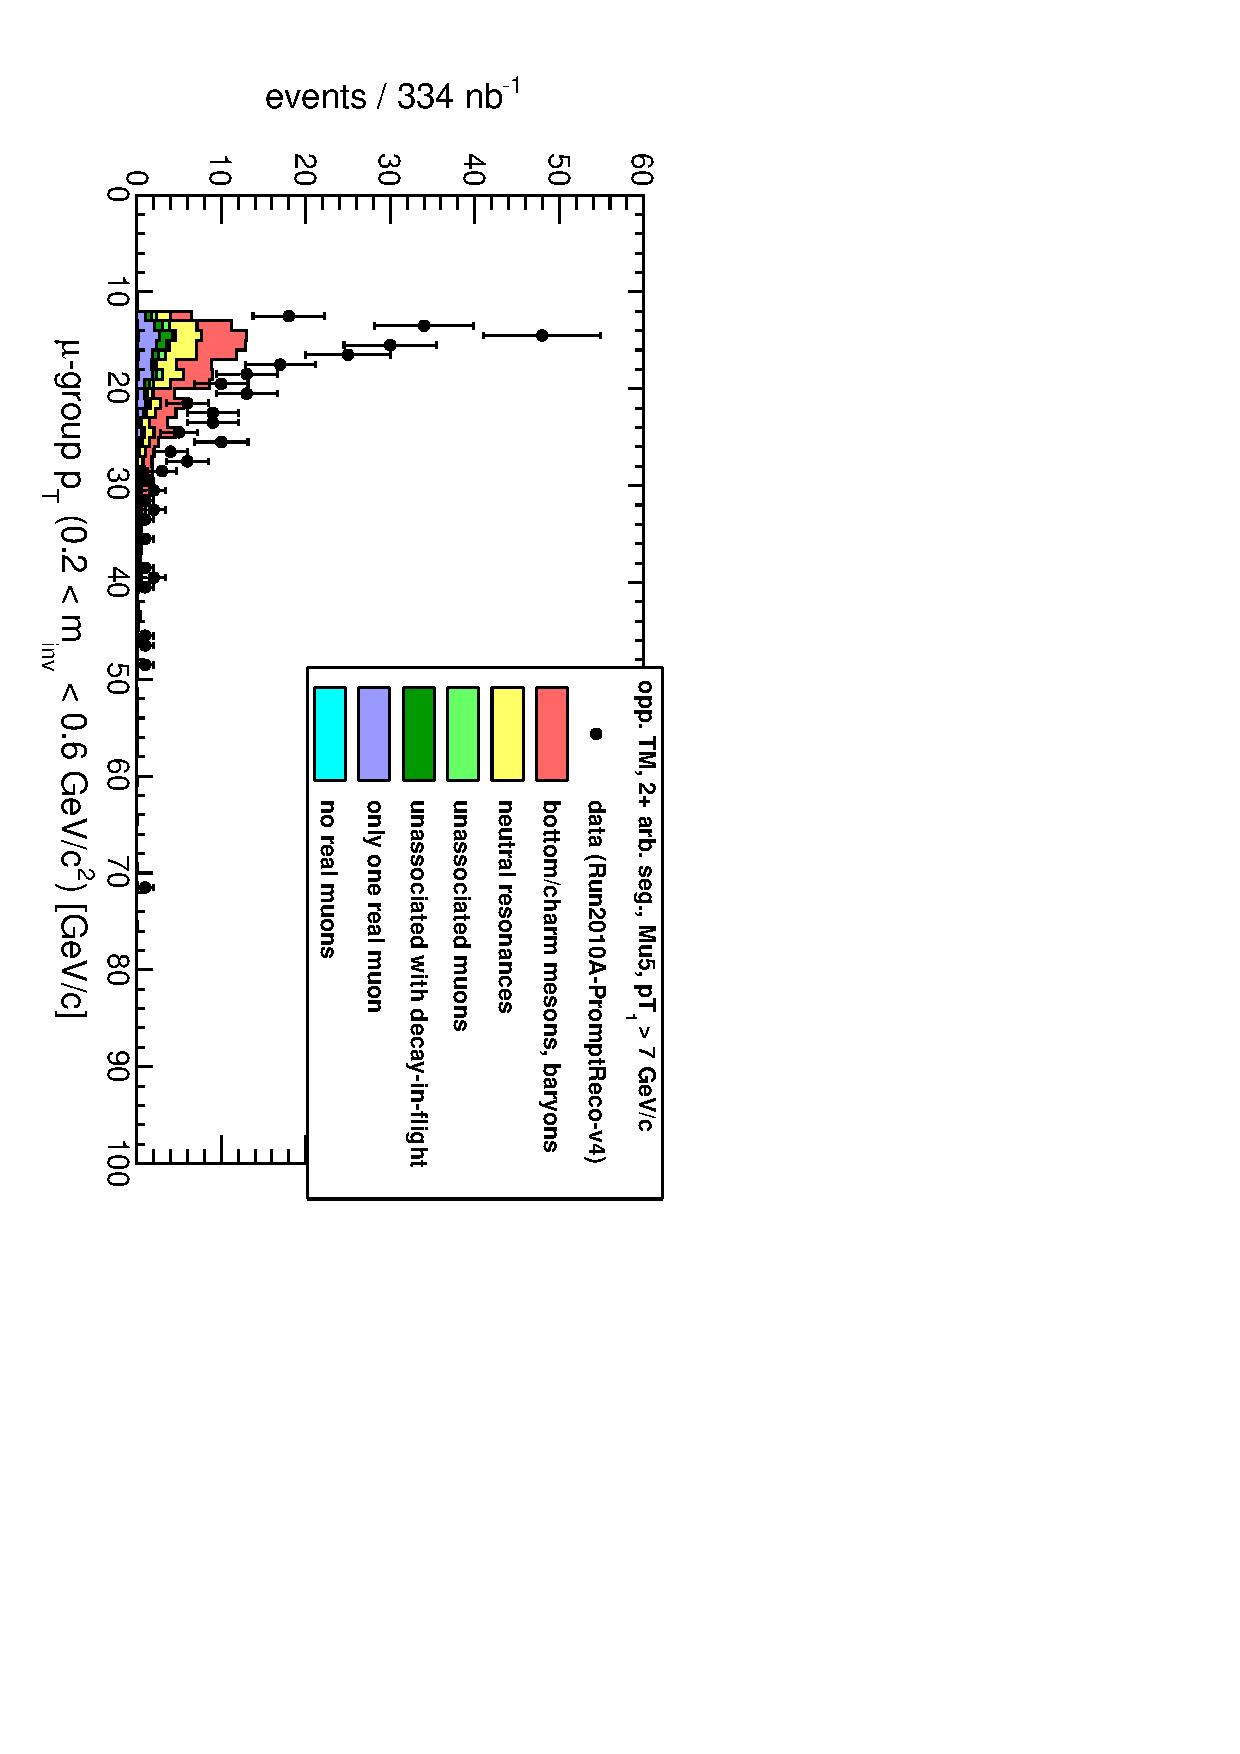
\includegraphics[height=\linewidth, angle=90]{Mu5_pt_eta.pdf}

\end{columns}
\end{frame}

\begin{frame}
\frametitle{Low-mass excess}

\begin{columns}
\column{0.6\linewidth}
\begin{itemize}
\item Excess of dimuons below 0.3~GeV/$c^2$ is not explained
\item Looked at all $\mathcal{O}(100)$ by hand: they're all
  good-looking muons

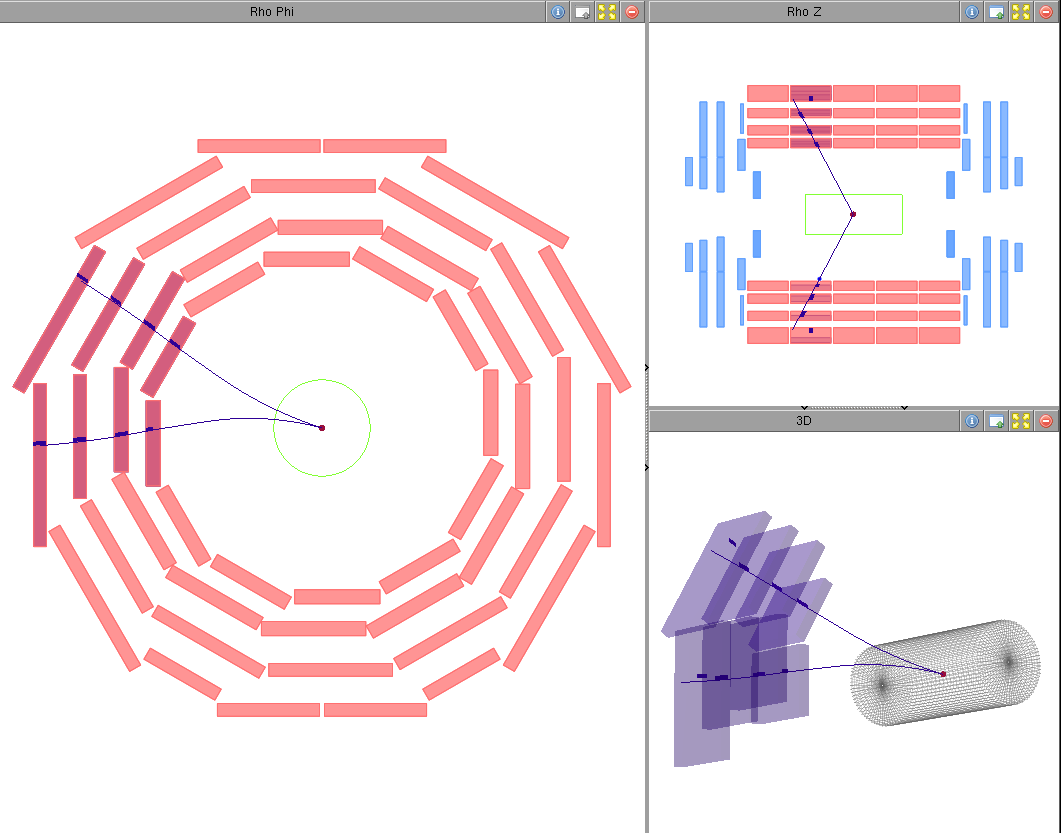
\includegraphics[width=\linewidth]{low-mass_perfectly-normal_2.png}

\item The dimuon vertices are not consistent with $\gamma X \to
  \mu^+\mu^- X$ \mbox{conversions (right)\hspace{-1 cm}}

\item Centrally distributed in $\eta$ \mbox{(not ME1/1a triplets)\hspace{-2 cm}}
\end{itemize}

\column{0.4\linewidth}
\begin{center}
{\scriptsize Vertex positions of $m_\s{inv} < 0.3$~GeV/$c^2$ events}

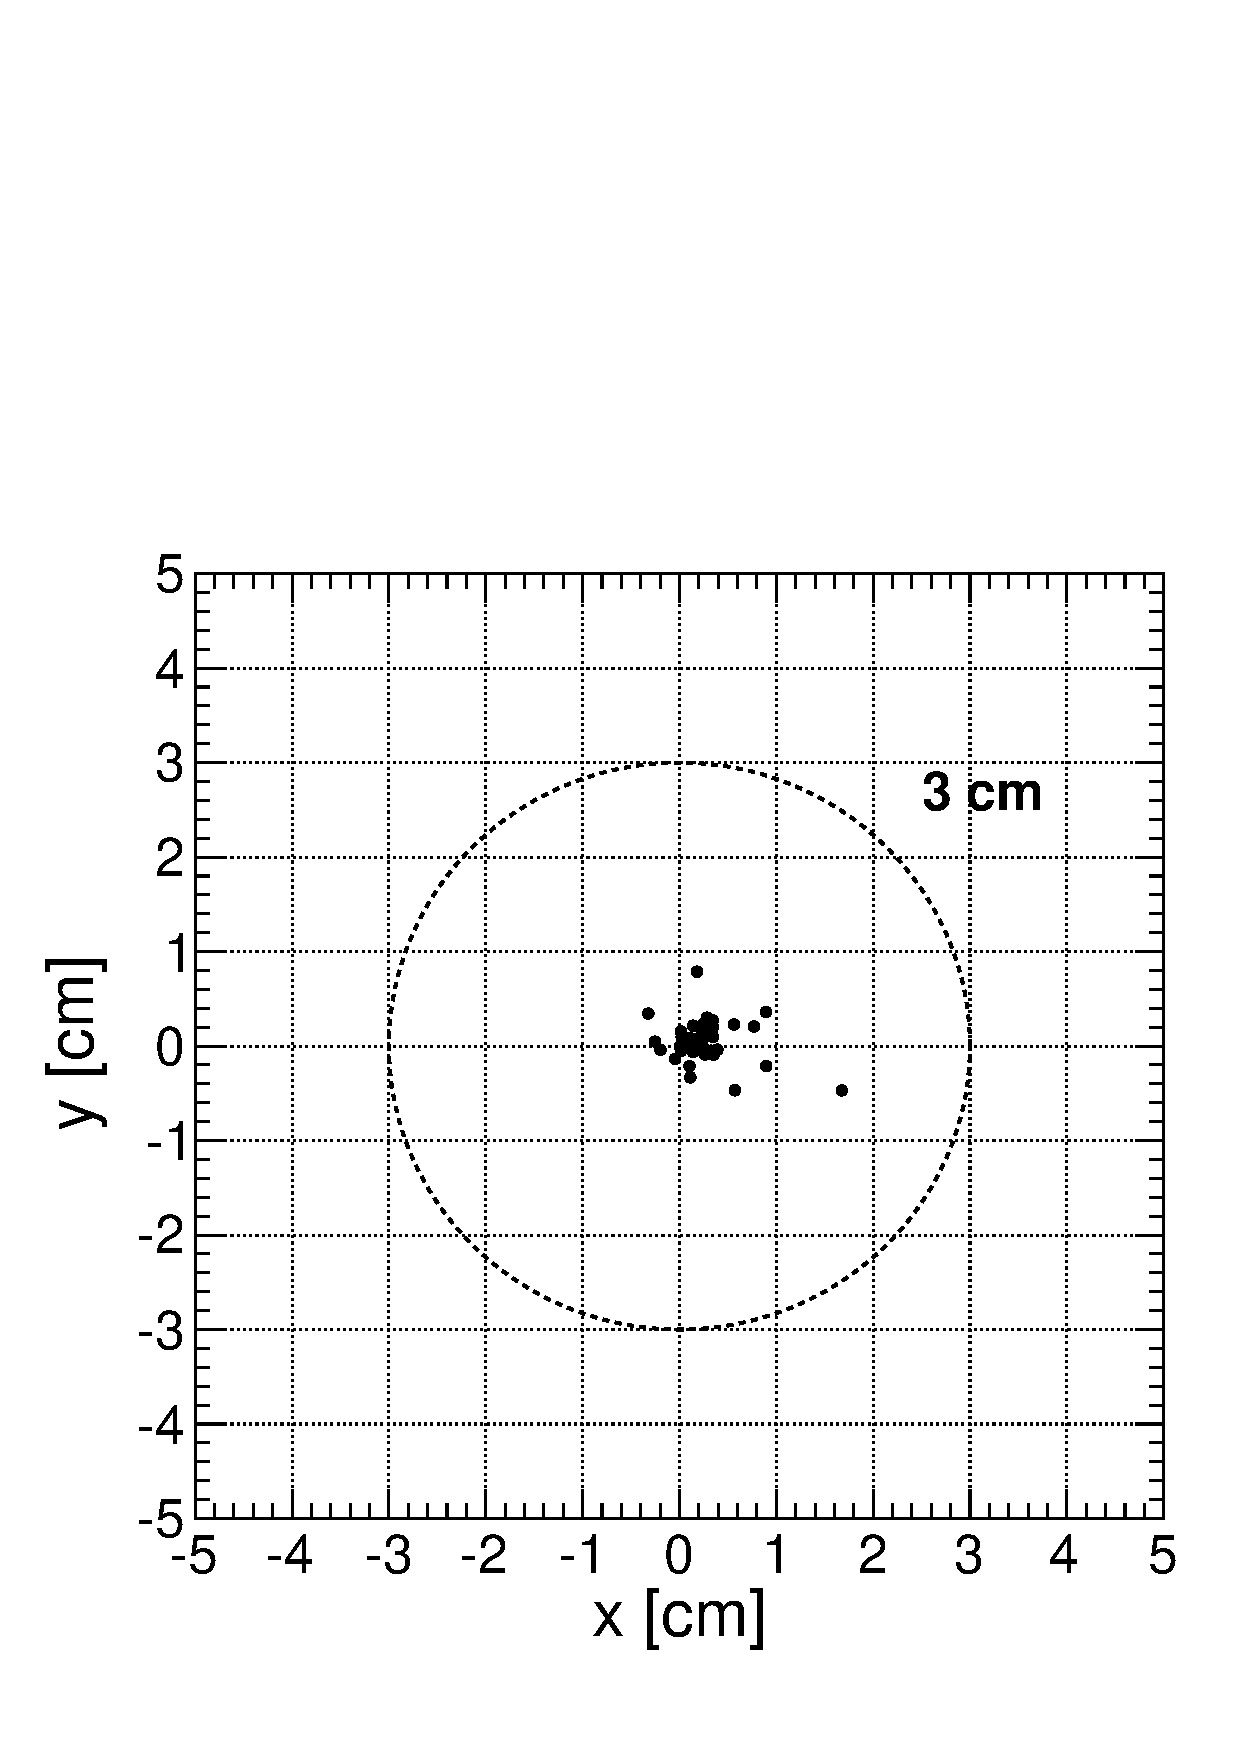
\includegraphics[width=0.7\linewidth]{Mu9_massbelow300MeV_vx_vy.pdf}

{\scriptsize $\gamma X \to e^+e^- X$ conversions (for~reference)}

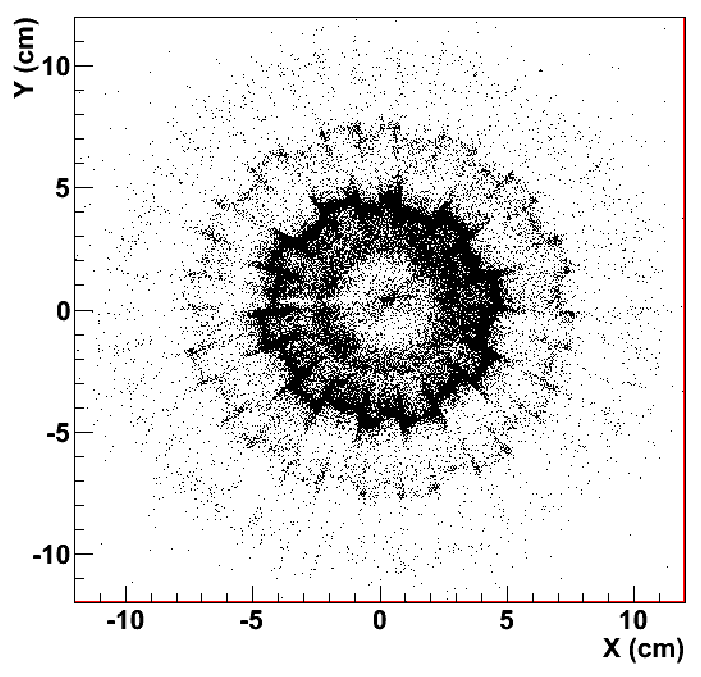
\includegraphics[width=0.7\linewidth]{electron_conversions.png}
\end{center}
\end{columns}
\end{frame}

% \section*{First section}
\begin{frame}
\begin{center}
\Huge \textcolor{blue}{Low-level quantities in 3\_8\_2}
\end{center}
\end{frame}

\begin{frame}
\frametitle{Low-level data/MC comparison}

\begin{itemize}\setlength{\itemsep}{0.1 cm}
\item Start with segment/propagated track comparisons to check for
  detector effects; later, work upward to kinematics again
\item Avoiding trigger bias: only look at muons that were not solely
  responsible for the HLT\_Mu9 trigger
\item Using latest alignment GlobalTag and 3\_8\_2 algorithms
  (re-reconstructed all tracks from the hits in data and MC)
\item Check residuals (segment-minus-propagated track) as a function of
\begin{itemize}\setlength{\itemsep}{0.2 cm}
\item \textcolor{darkblue}{inverse momentum ($q/p_T$ or $q/|p|$):} sensitive to propagation issues (e.g.\ $\vec{B}$-field bias, material budget)
\item \textcolor{darkblue}{wheel/disk/station:} sensitive to misalignment
\end{itemize}
\item Four segment/propagated track parameters:
\begin{itemize}
\item $x$: local coordinate equivalent to $r\phi$; \mbox{``$\phi$ residual'' = $x/R_\s{chamber}$\hspace{-1 cm}}
\item $y$: parallel to beamline (DT) or radial (CSC)
\item $dx/dz$ (entrance angle in bending plane)
\item $dy/dz$
\end{itemize}
\end{itemize}
\end{frame}

\begin{frame}
\frametitle{Dependence on momentum}

\begin{columns}
\column{0.4\linewidth}
\begin{itemize}
\item Plot $\phi$ residuals from MB3 and ME2 only

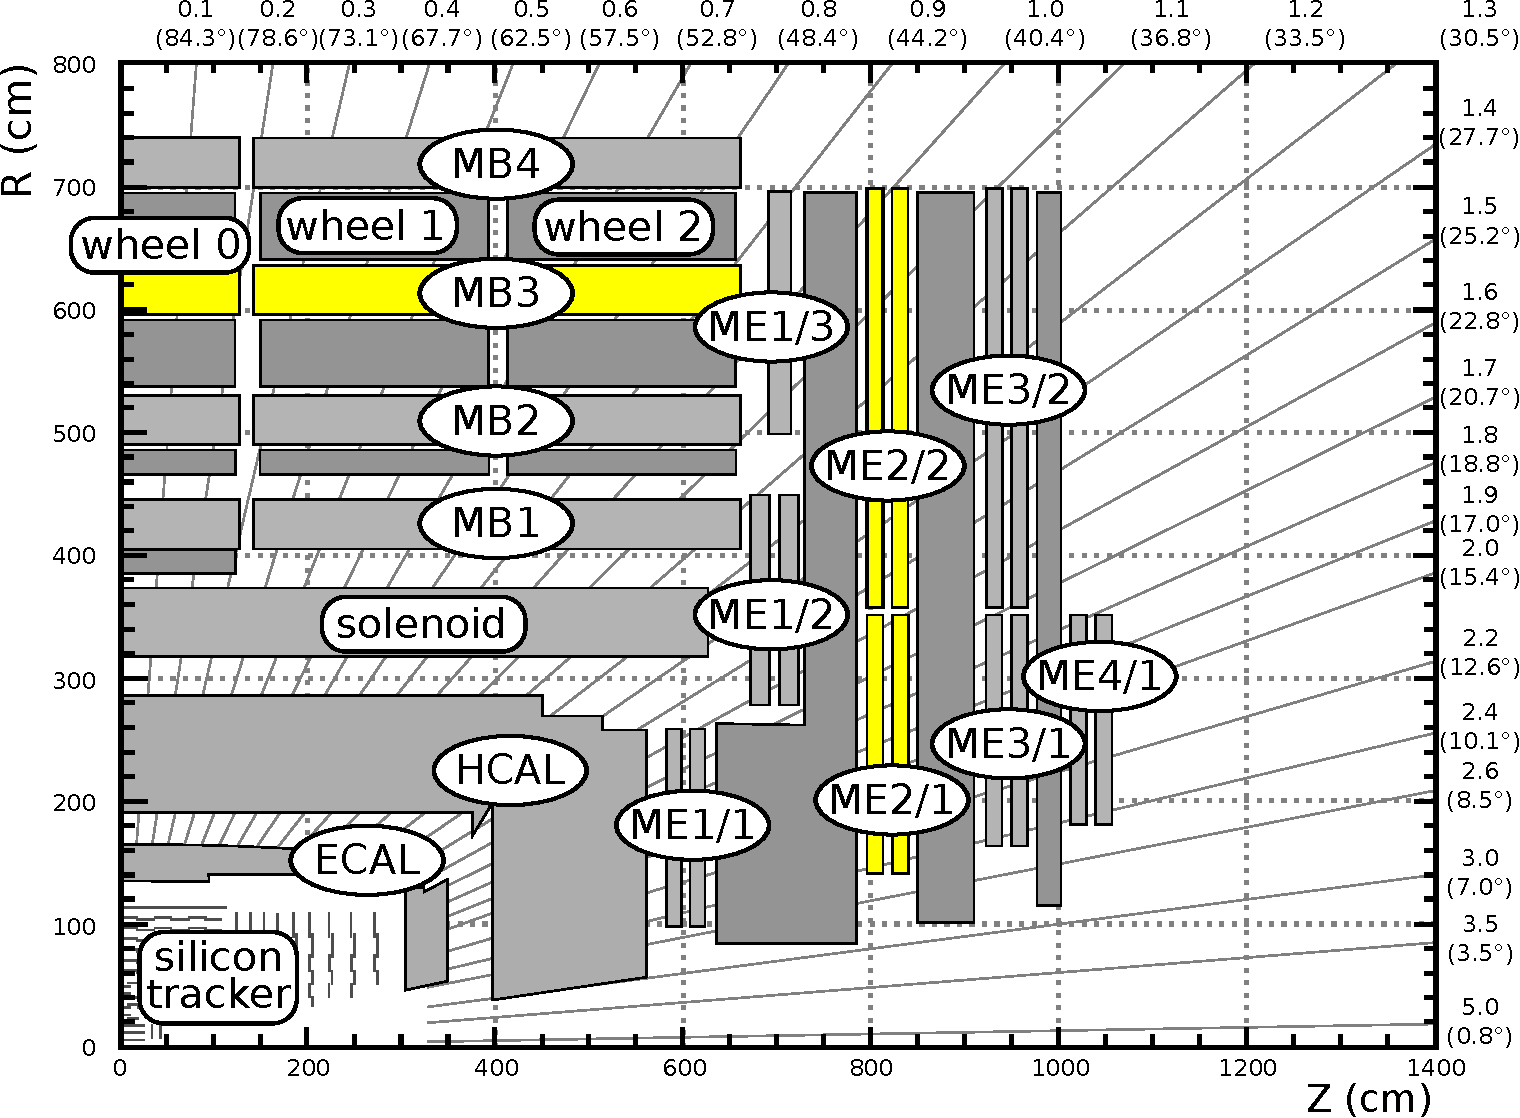
\includegraphics[width=\linewidth]{muon_system_labeled_mb3-me2.pdf}

(one representative residual per track)

\item Width of residuals distribution scales roughly as $1/|p|$, cut at $1/p_T < 0.2$~$c$/GeV

\item Any biases in the mean are much smaller than the width of
  \mbox{the distribution\hspace{-1 cm}}
\end{itemize}

\column{0.6\linewidth}
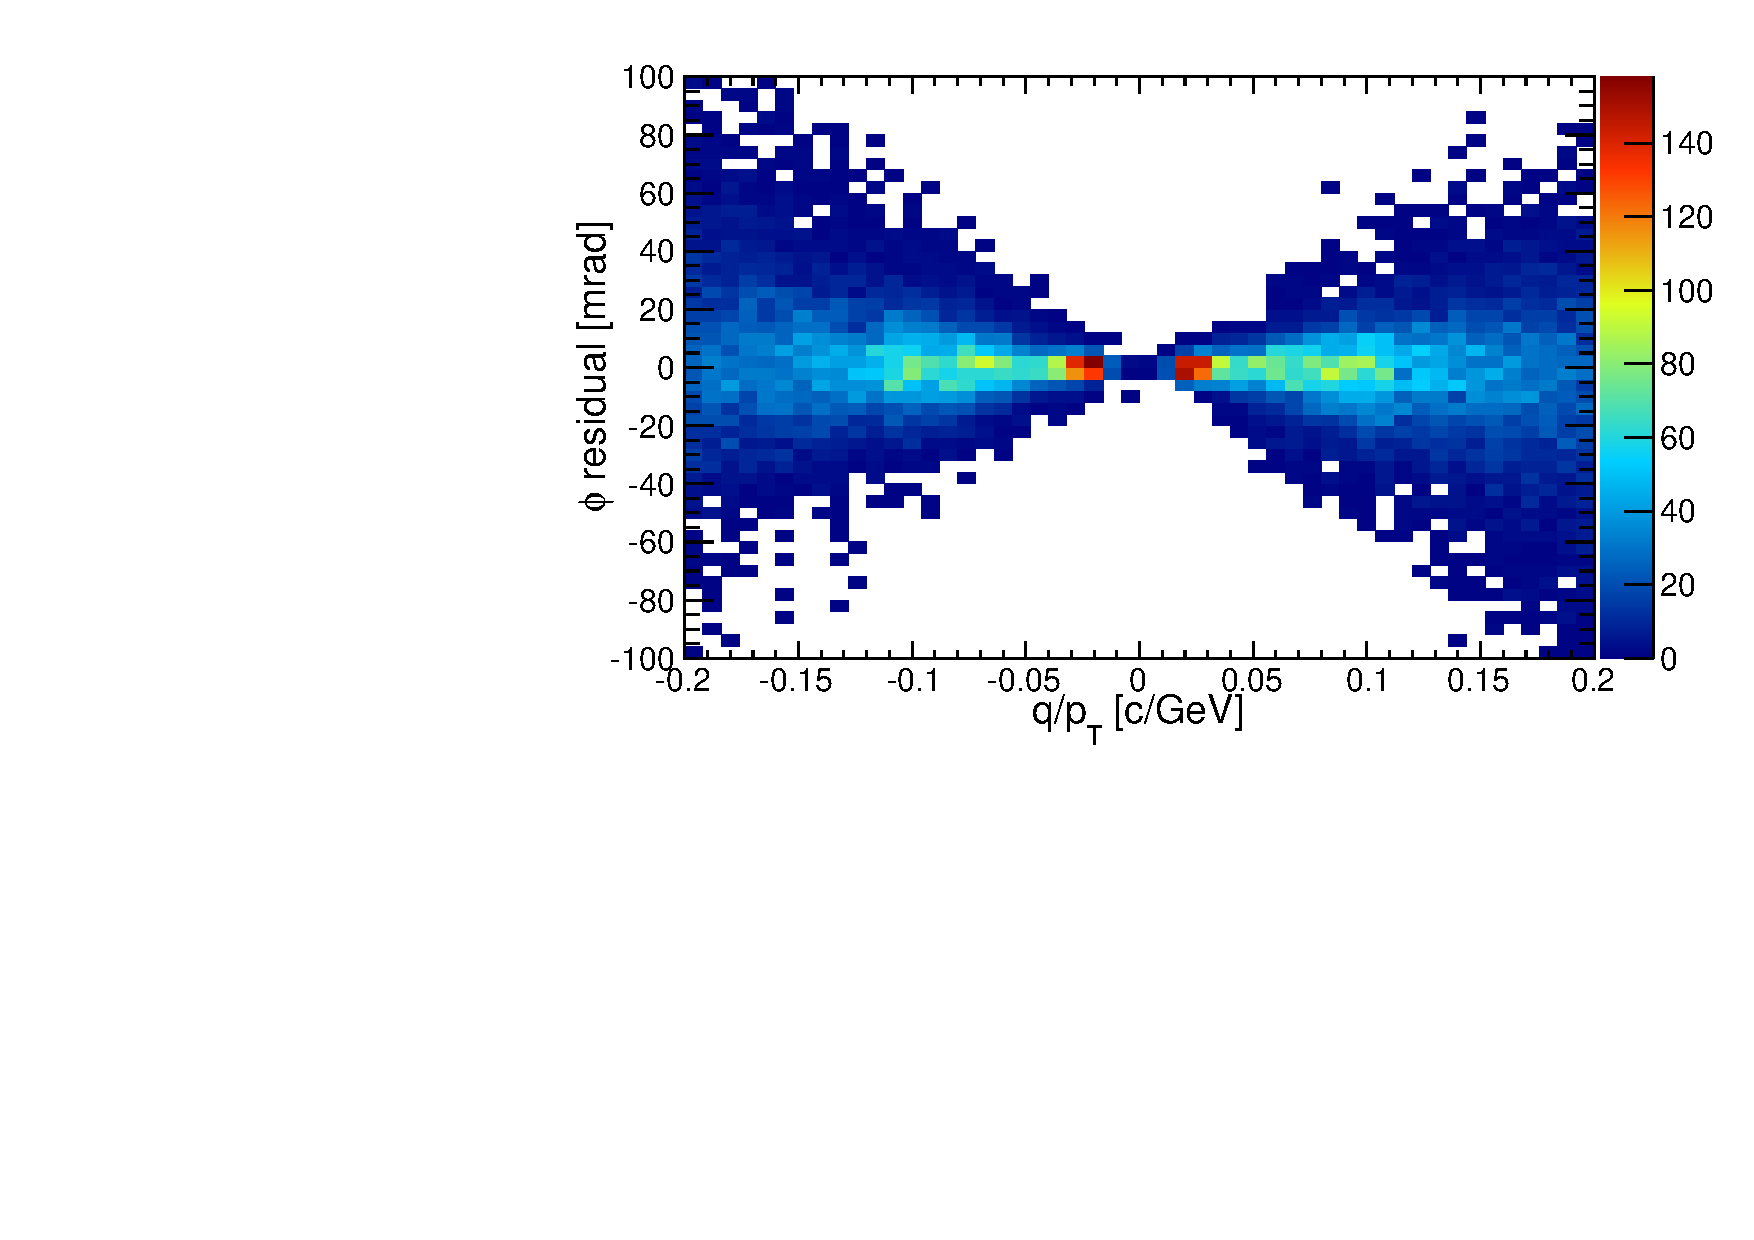
\includegraphics[width=\linewidth]{simple2d_qoverpt.pdf}

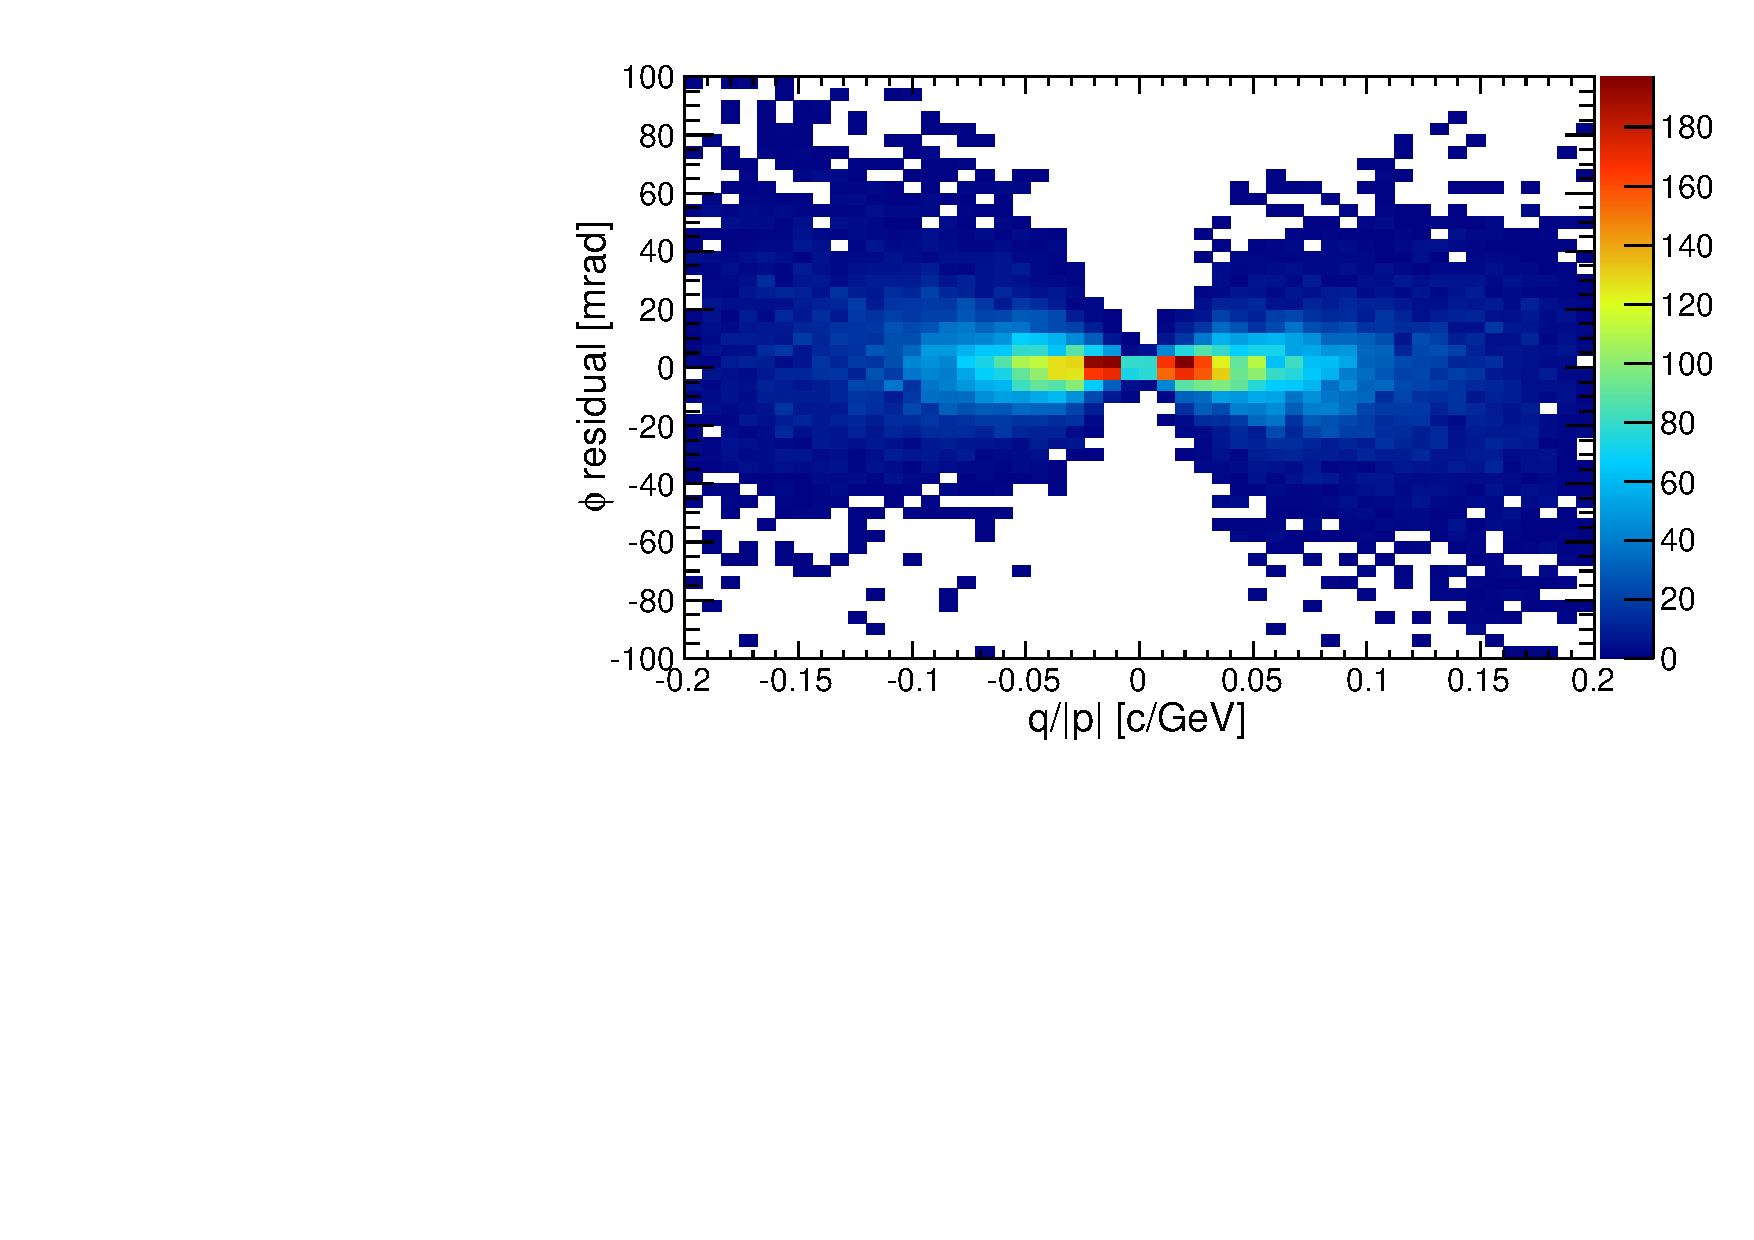
\includegraphics[width=\linewidth]{simple2d_qoverpmag.pdf}
\end{columns}
\end{frame}

\begin{frame}
\frametitle{Dependence on momentum}

\vspace{-1.8 cm}
\begin{itemize}
\item To quantify bias in the Gaussian part of the residuals peak (not
  the tails), fit distributions in momentum bins to
\[ p(x) = \left\{ \begin{array}{c c}
A \exp\left(-(x - x_0)^2/(2\sigma^2)\right) & |x - x_0| < m \\
B/|x|^{p_1} & (x - x_0) > m_1 \\
C/|x|^{p_2} & -(x - x_0) < -m_2 \\
\end{array} \right. \]

where $A$, $B$, $C$, $m_1$, and $m_2$ are chosen to make the function
continuous and differentiable
\end{itemize}

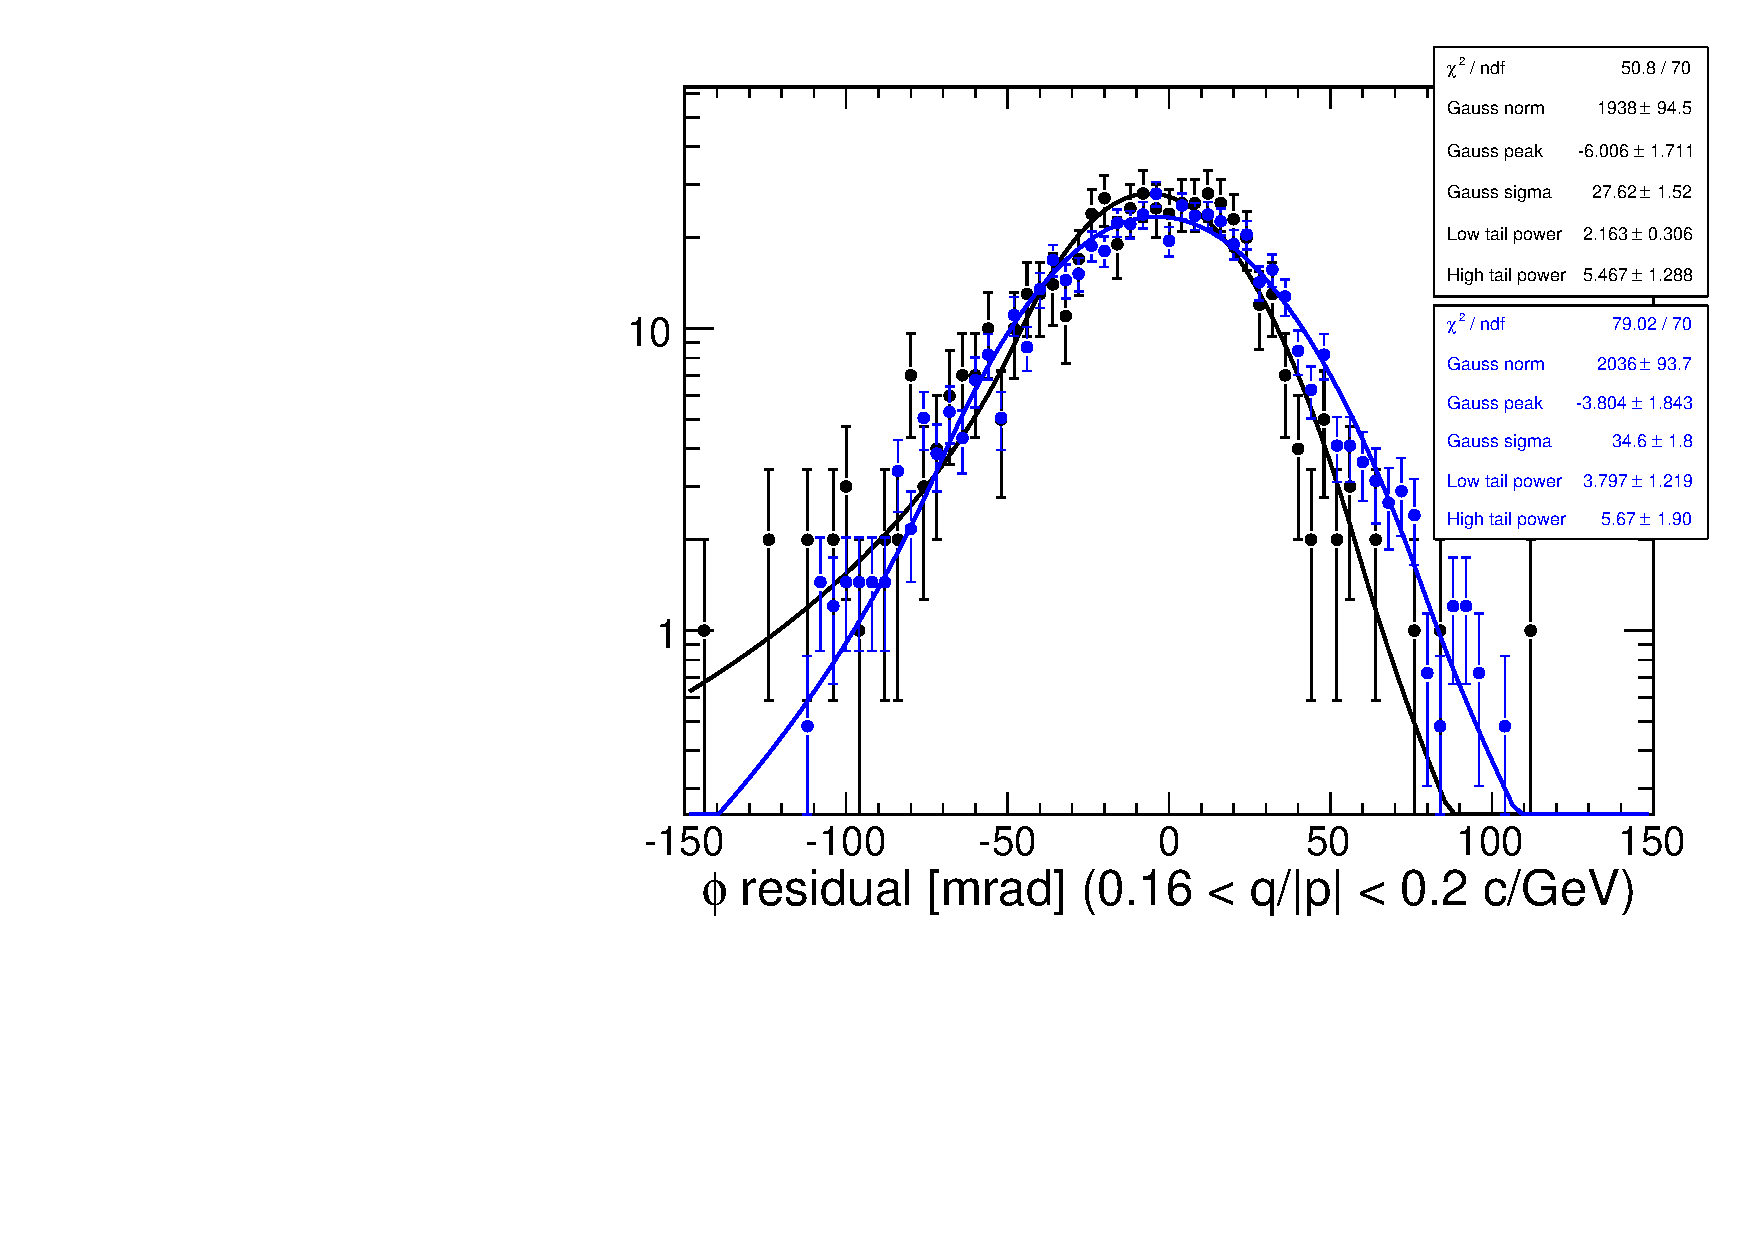
\includegraphics[width=0.49\linewidth]{example_lowmomentum.pdf}
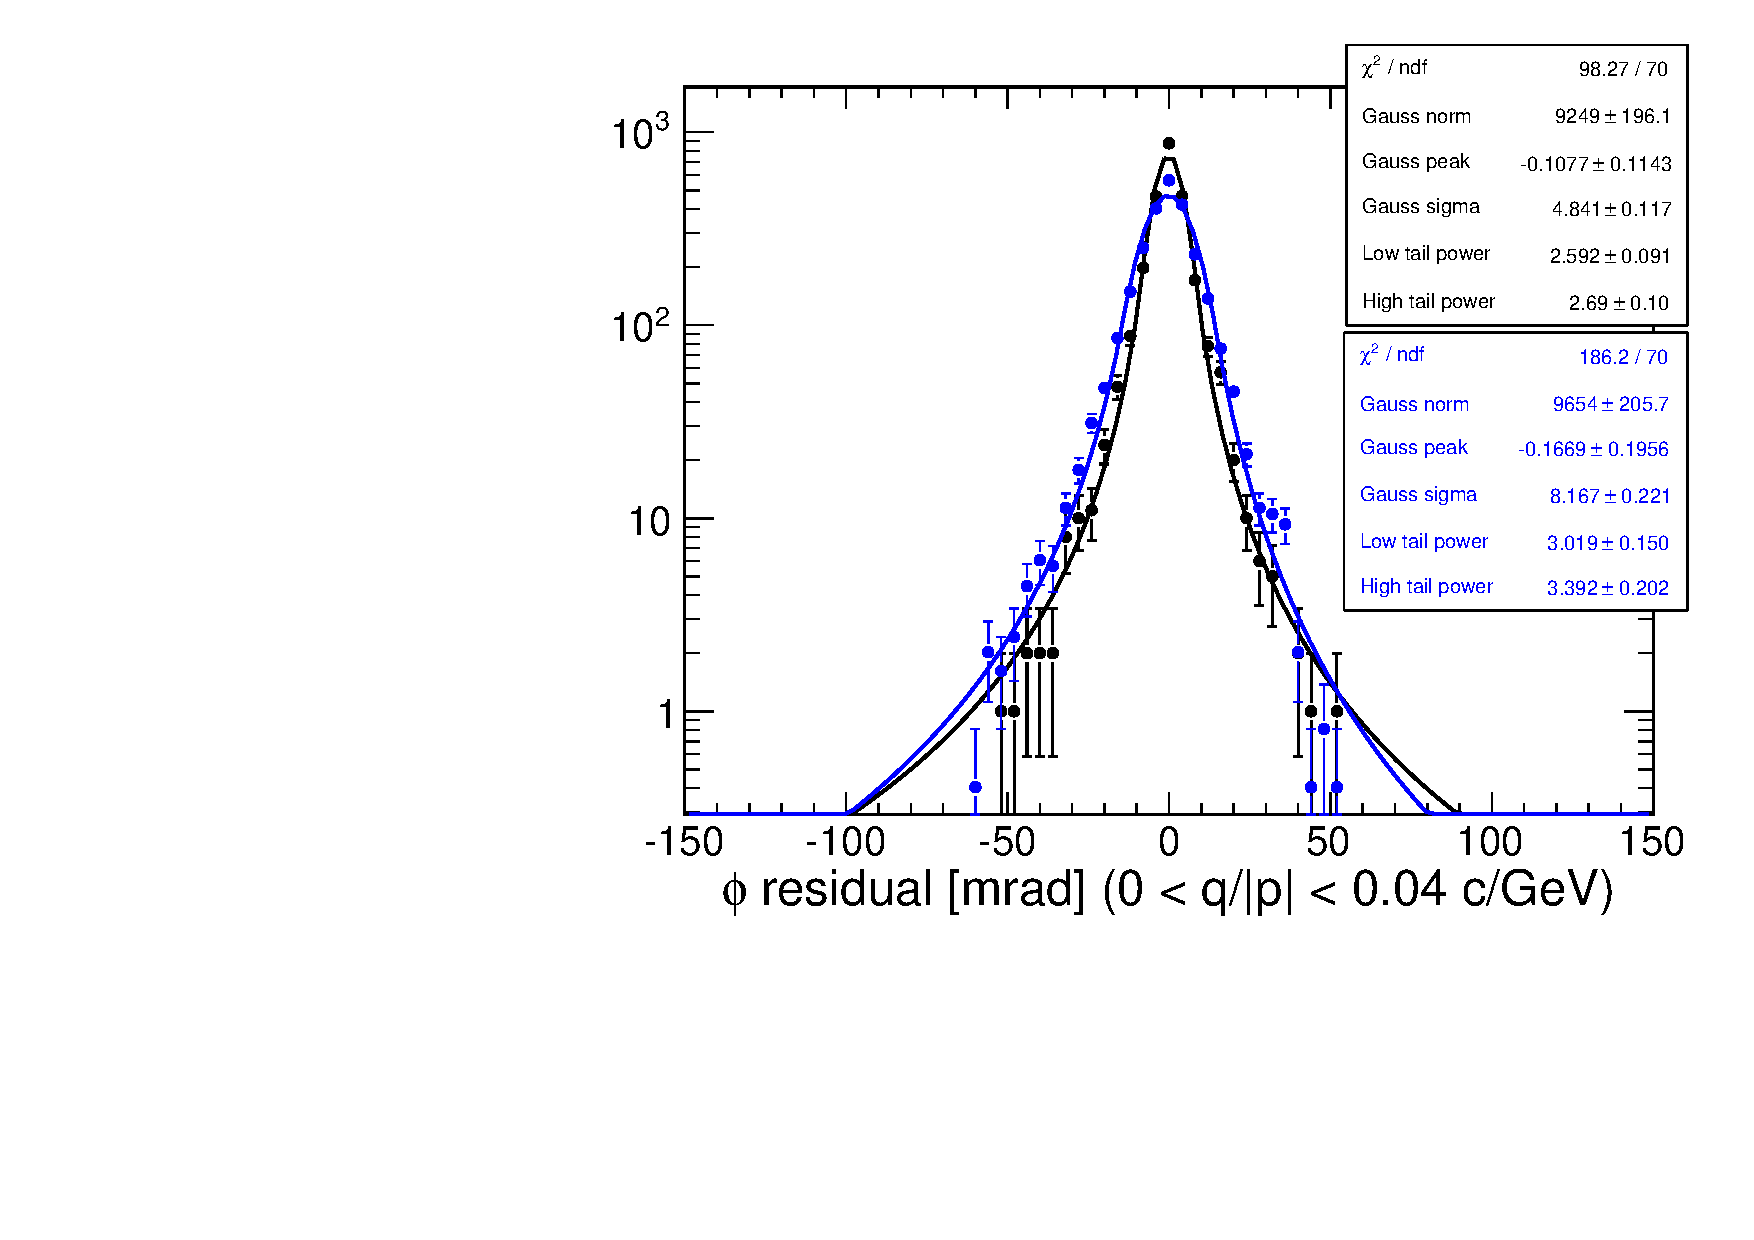
\includegraphics[width=0.49\linewidth]{example_highmomentum.pdf}

\vspace{-3.6 cm}
\hspace{6.3 cm}\textcolor{black}{data: black}

\hspace{6.3 cm}\textcolor{blue}{MC: blue}
\end{frame}

\begin{frame}
\frametitle{Dependence on momentum}
\begin{itemize}
\item Slope of Gaussian peak vs.\ $q/|p|$ obscured by decays-in-flight
\begin{itemize}\setlength{\itemsep}{0.2 cm}
\item \textcolor{darkgreen}{Green}: all muons (TM with $p_T > 5$~GeV/$c$ and $N_\s{segments} \ge 2$)
\item \textcolor{black}{Black:} excluding muons matched to decay-in-flight (MC only)
\item \textcolor{red}{Red:} member of $\mu$-group ($P_\s{vertex} > 1\%$ with another muon)
\item \textcolor{blue}{Blue:} within 0.2~GeV/$c^2$ of $J/\psi$ peak (very pure muons)
\end{itemize}
\item Removing that, there's a bias in data not present in Monte Carlo
\end{itemize}

\vspace{-0.5 cm}
\begin{columns}
\column{0.5\linewidth}
\begin{center} Data \end{center}

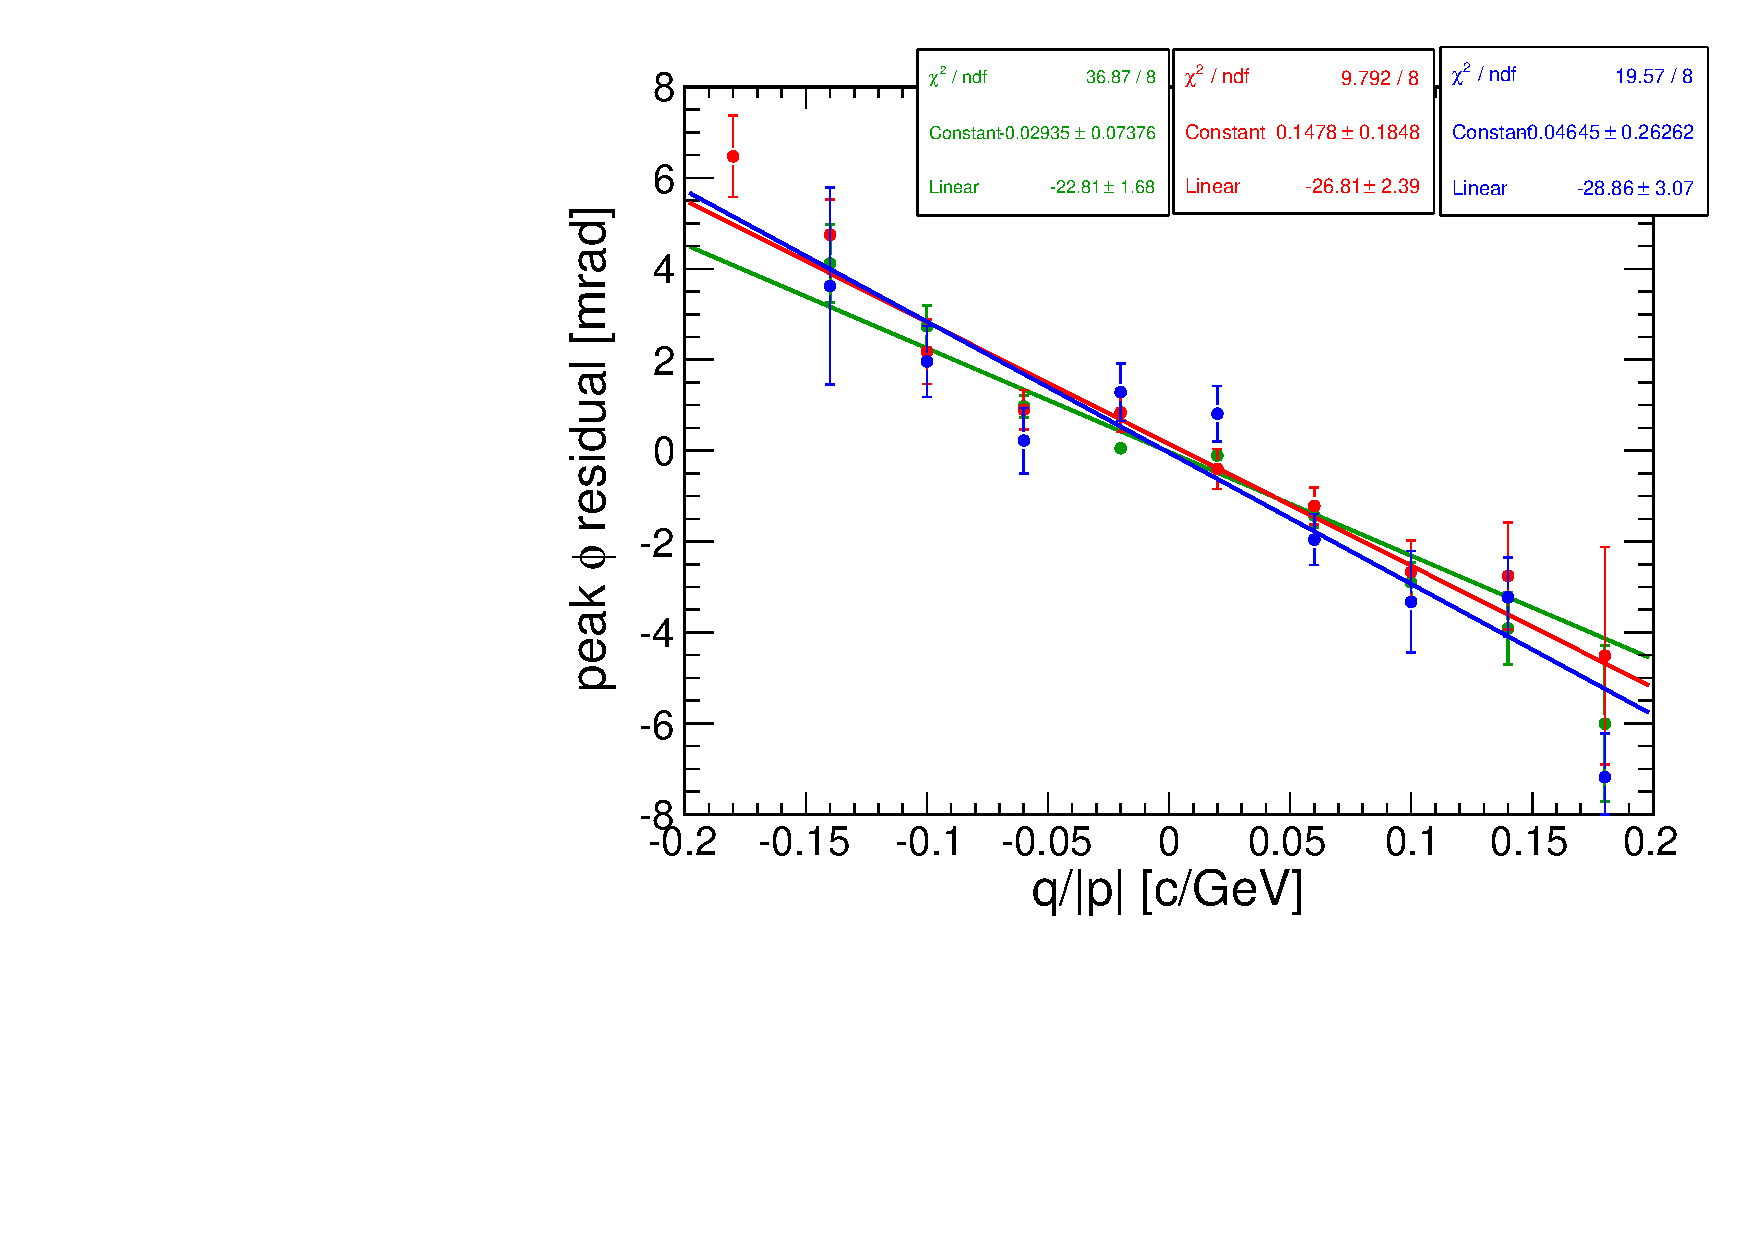
\includegraphics[width=\linewidth]{datacuts_allmu_ingroup_jpsi.pdf}
\column{0.5\linewidth}
\begin{center} Monte Carlo \end{center}

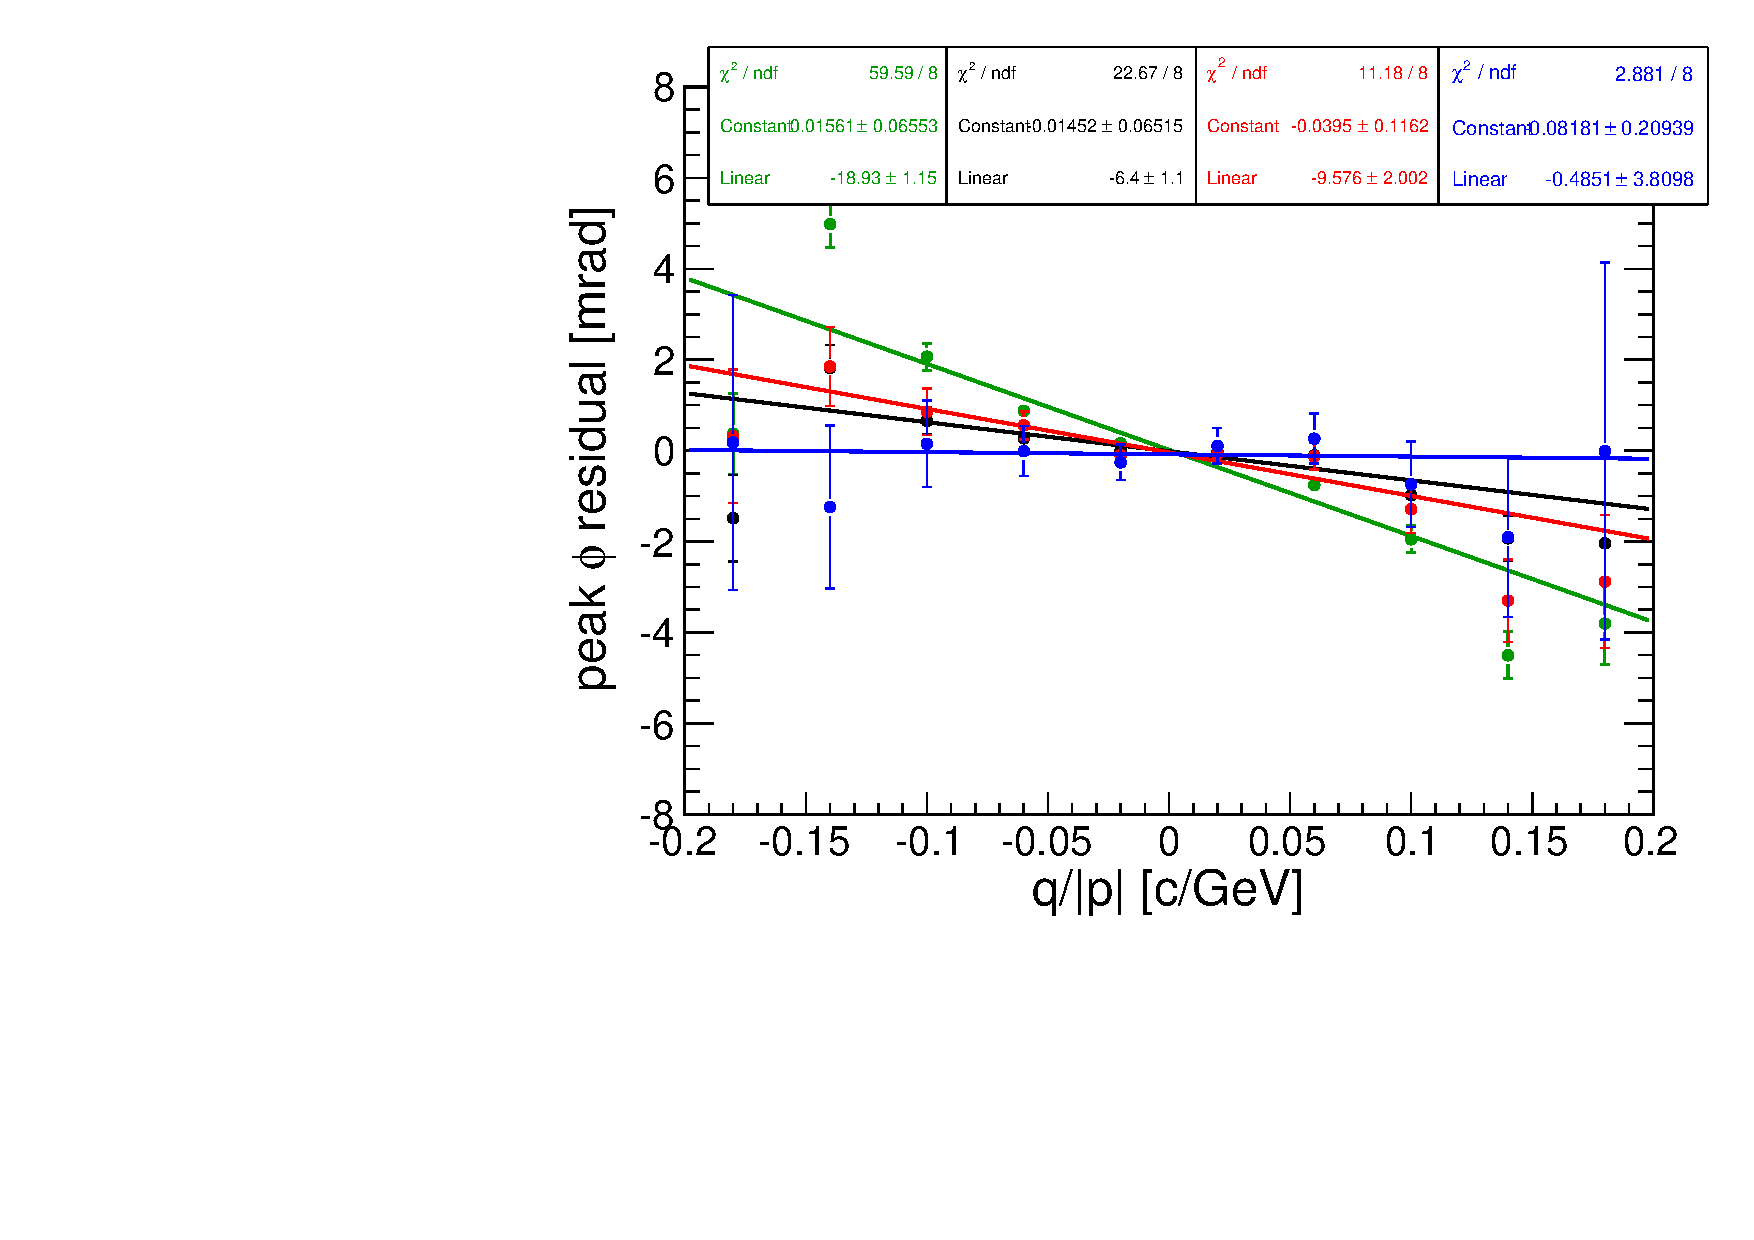
\includegraphics[width=\linewidth]{mccuts_allmu_noinfly_ingroup_jpsi.pdf}
\end{columns}
\end{frame}

\begin{frame}
\frametitle{Dependence on momentum}
\begin{itemize}
\item Re-drawing residual vs.\ $q/p_T$ and $q/|p|$ for muons from $J/\psi$

\textcolor{red}{data in red}, \textcolor{blue}{Monte Carlo in blue}

\begin{itemize}\setlength{\itemsep}{0.1 cm}
\item trend is stronger vs.\ $q/|p|$ (but that might be different
  influence of the endcap detectors relative to the barrel)

\item bias is about 15\% of the width of the distribution at 5~GeV/$c$
\end{itemize}

\item Modifying dE/dx in SteppingHelixPropagator tunes this plot

(but I don't plan to apply an ad-hoc tune)
\end{itemize}

\vfill
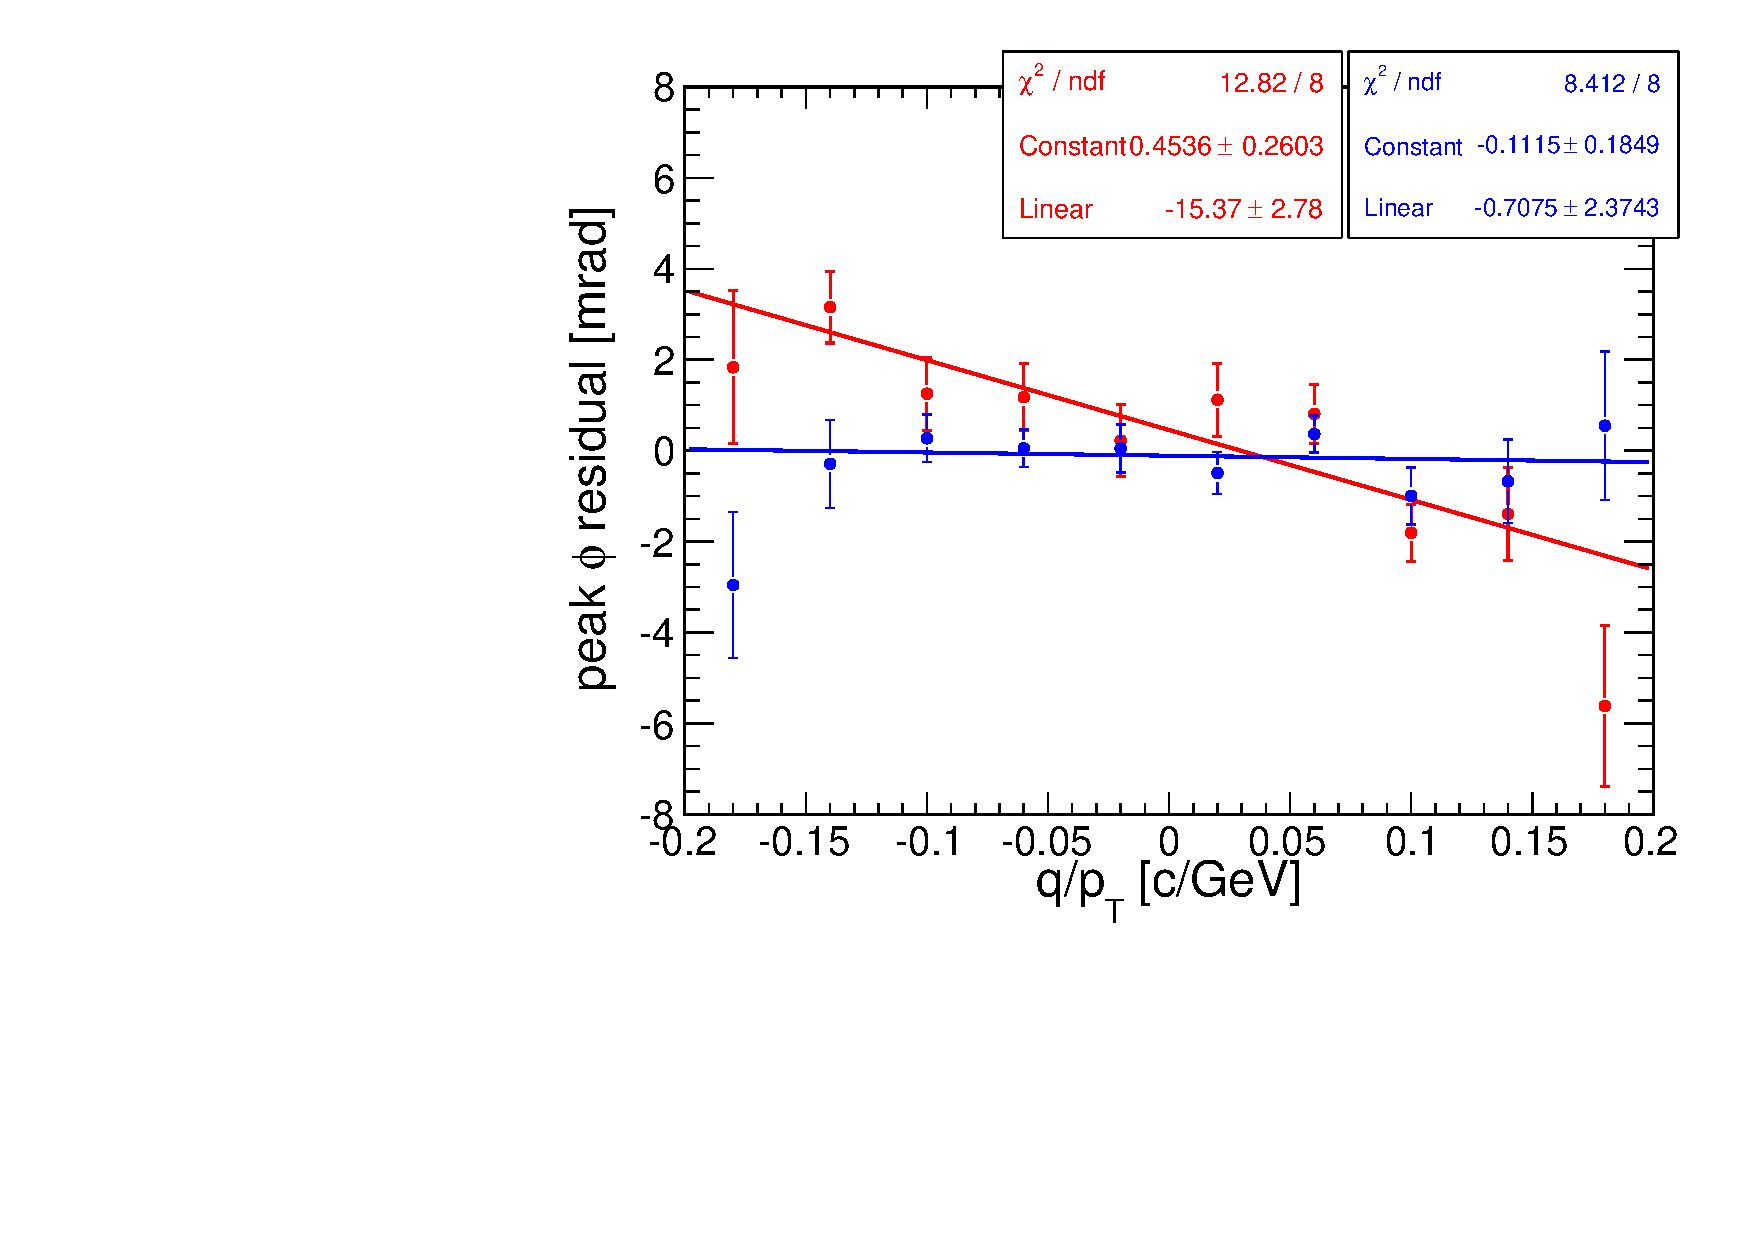
\includegraphics[width=0.49\linewidth]{datamc_jpsicut_qoverpt.pdf}
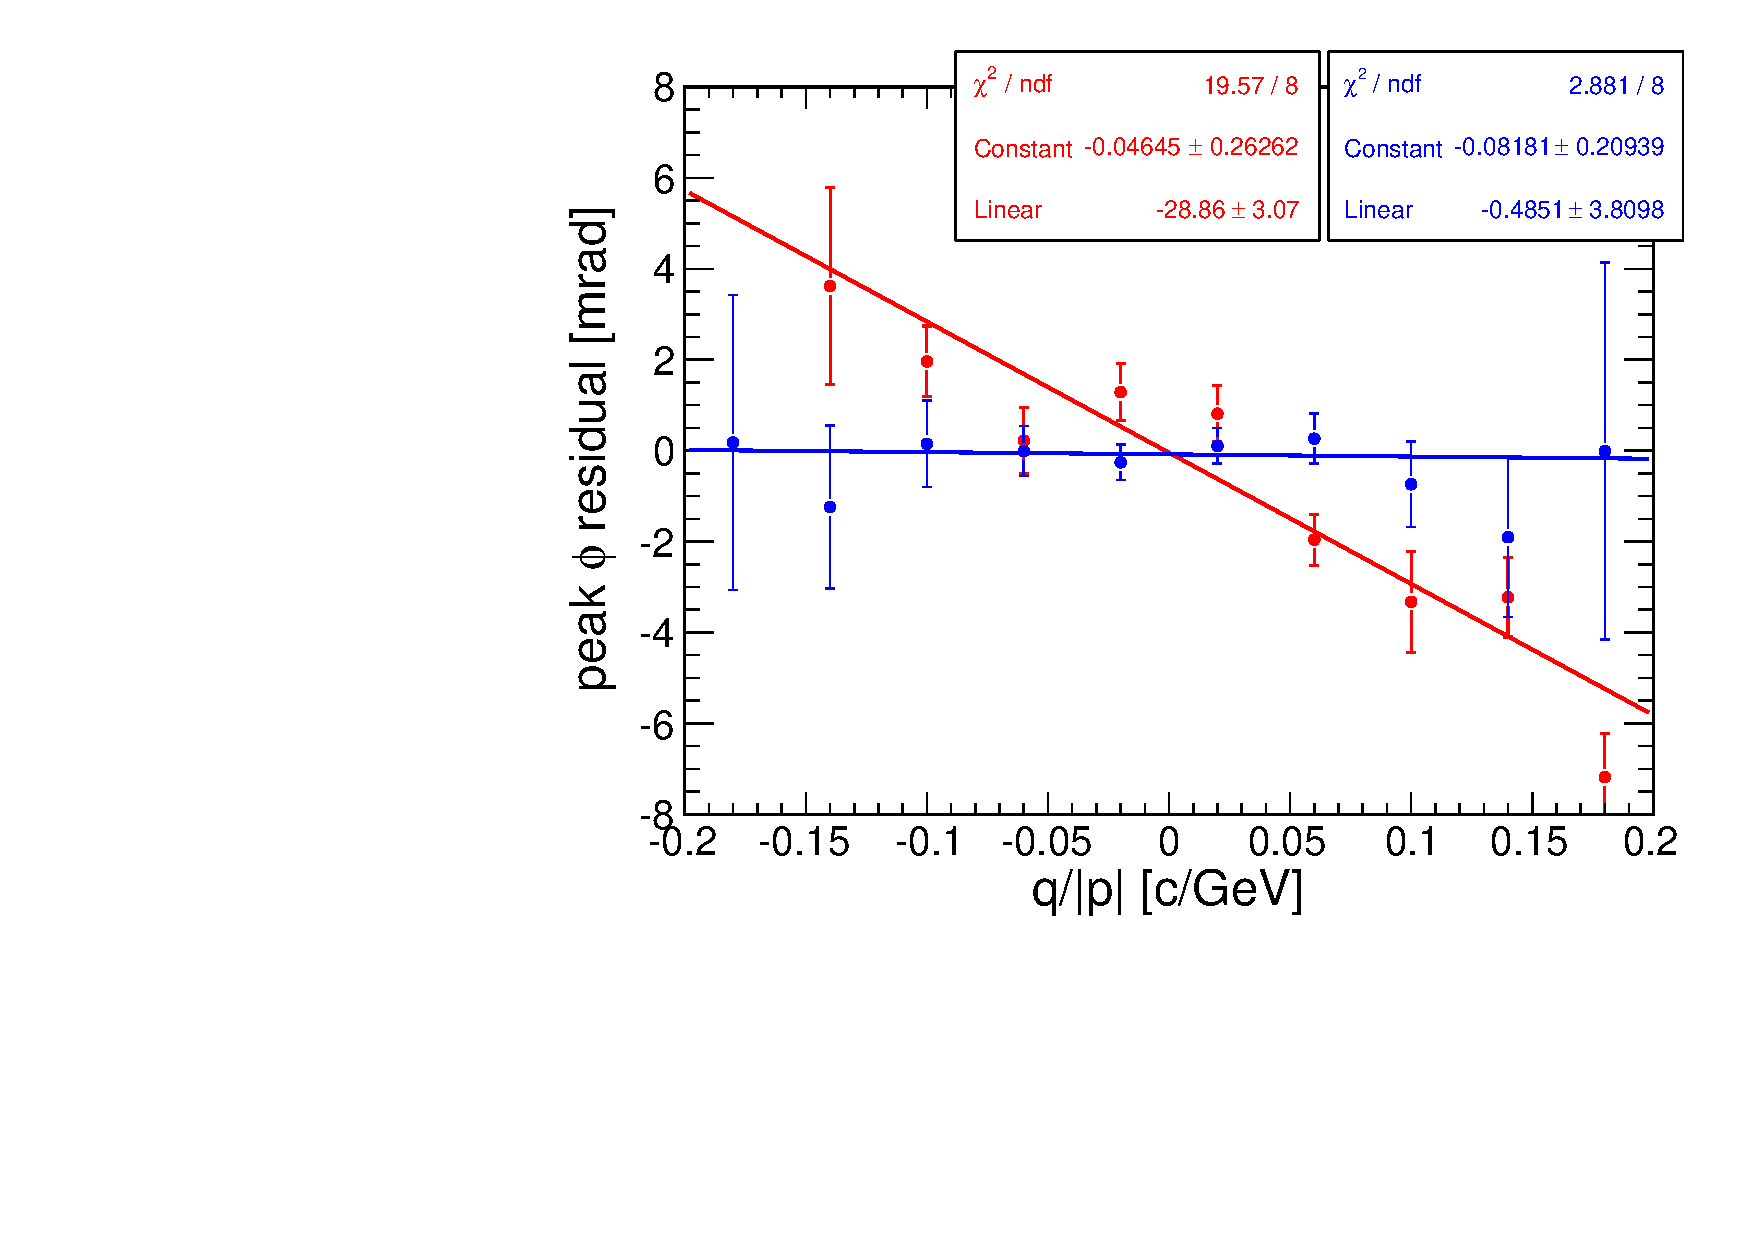
\includegraphics[width=0.49\linewidth]{datamc_jpsicut_qoverpmag.pdf}
\end{frame}

\begin{frame}
\frametitle{Dependence on detectors}

\begin{itemize}
\item Plot four components of residuals ($x$, $y$, $dx/dz$, $dy/dz$) for
  each distinct ring of detectors
\begin{itemize}
\item barrel wheels 0, $\pm$1, $\pm$2 and stations 1, 2, 3, 4
\item endcap stations 1/1, 1/2, 1/3, 2/1, 2/2, 3/1, 3/2, 4/1, 4/2
\end{itemize}
\item No trigger bias (only look at muons not solely responsible for
  HLT\_Mu9 trigger)
\item Select only muons in $\mu$-groups (similar results in $J/\psi$-only)
\item Examples (points are data, shaded blue/grey is Monte Carlo):
\end{itemize}

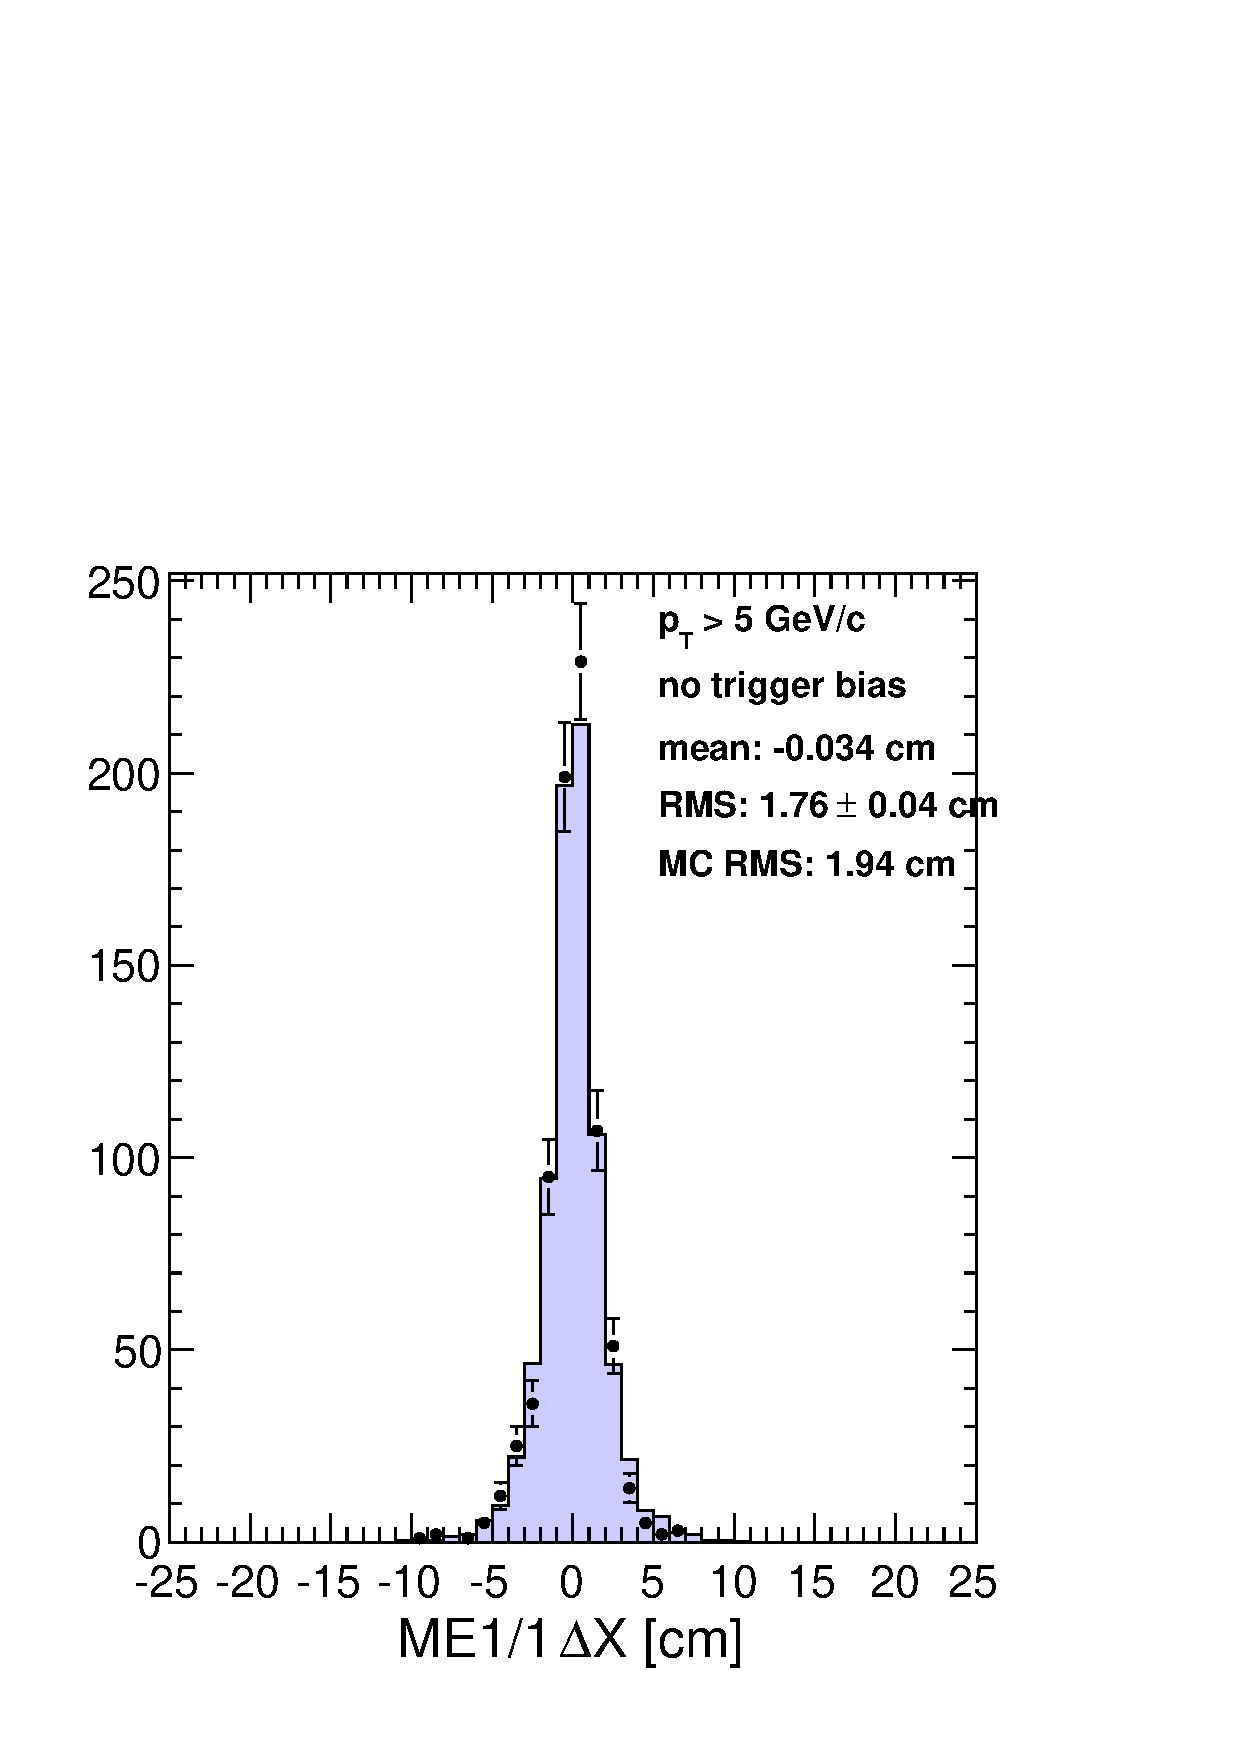
\includegraphics[width=0.24\linewidth]{me11_X.pdf}
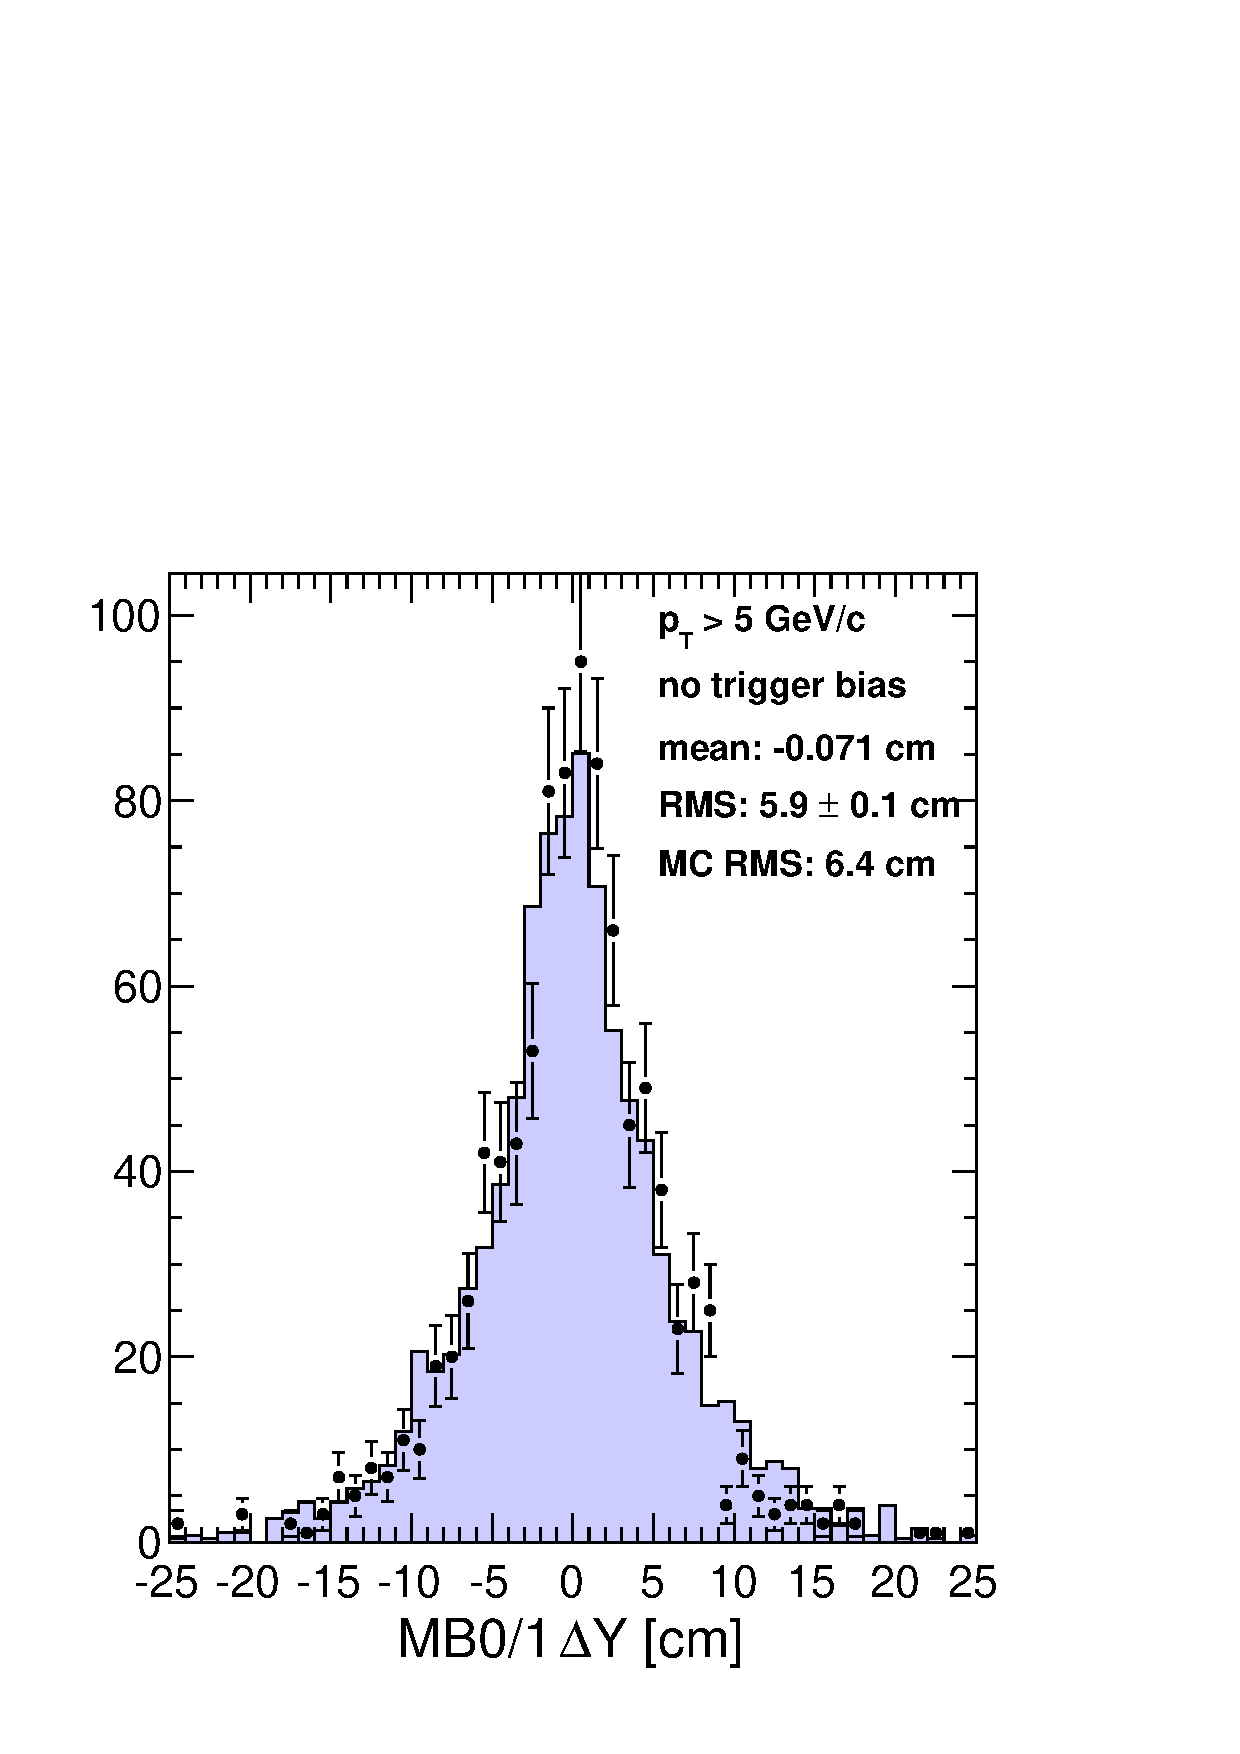
\includegraphics[width=0.24\linewidth]{mb01_Y.pdf}
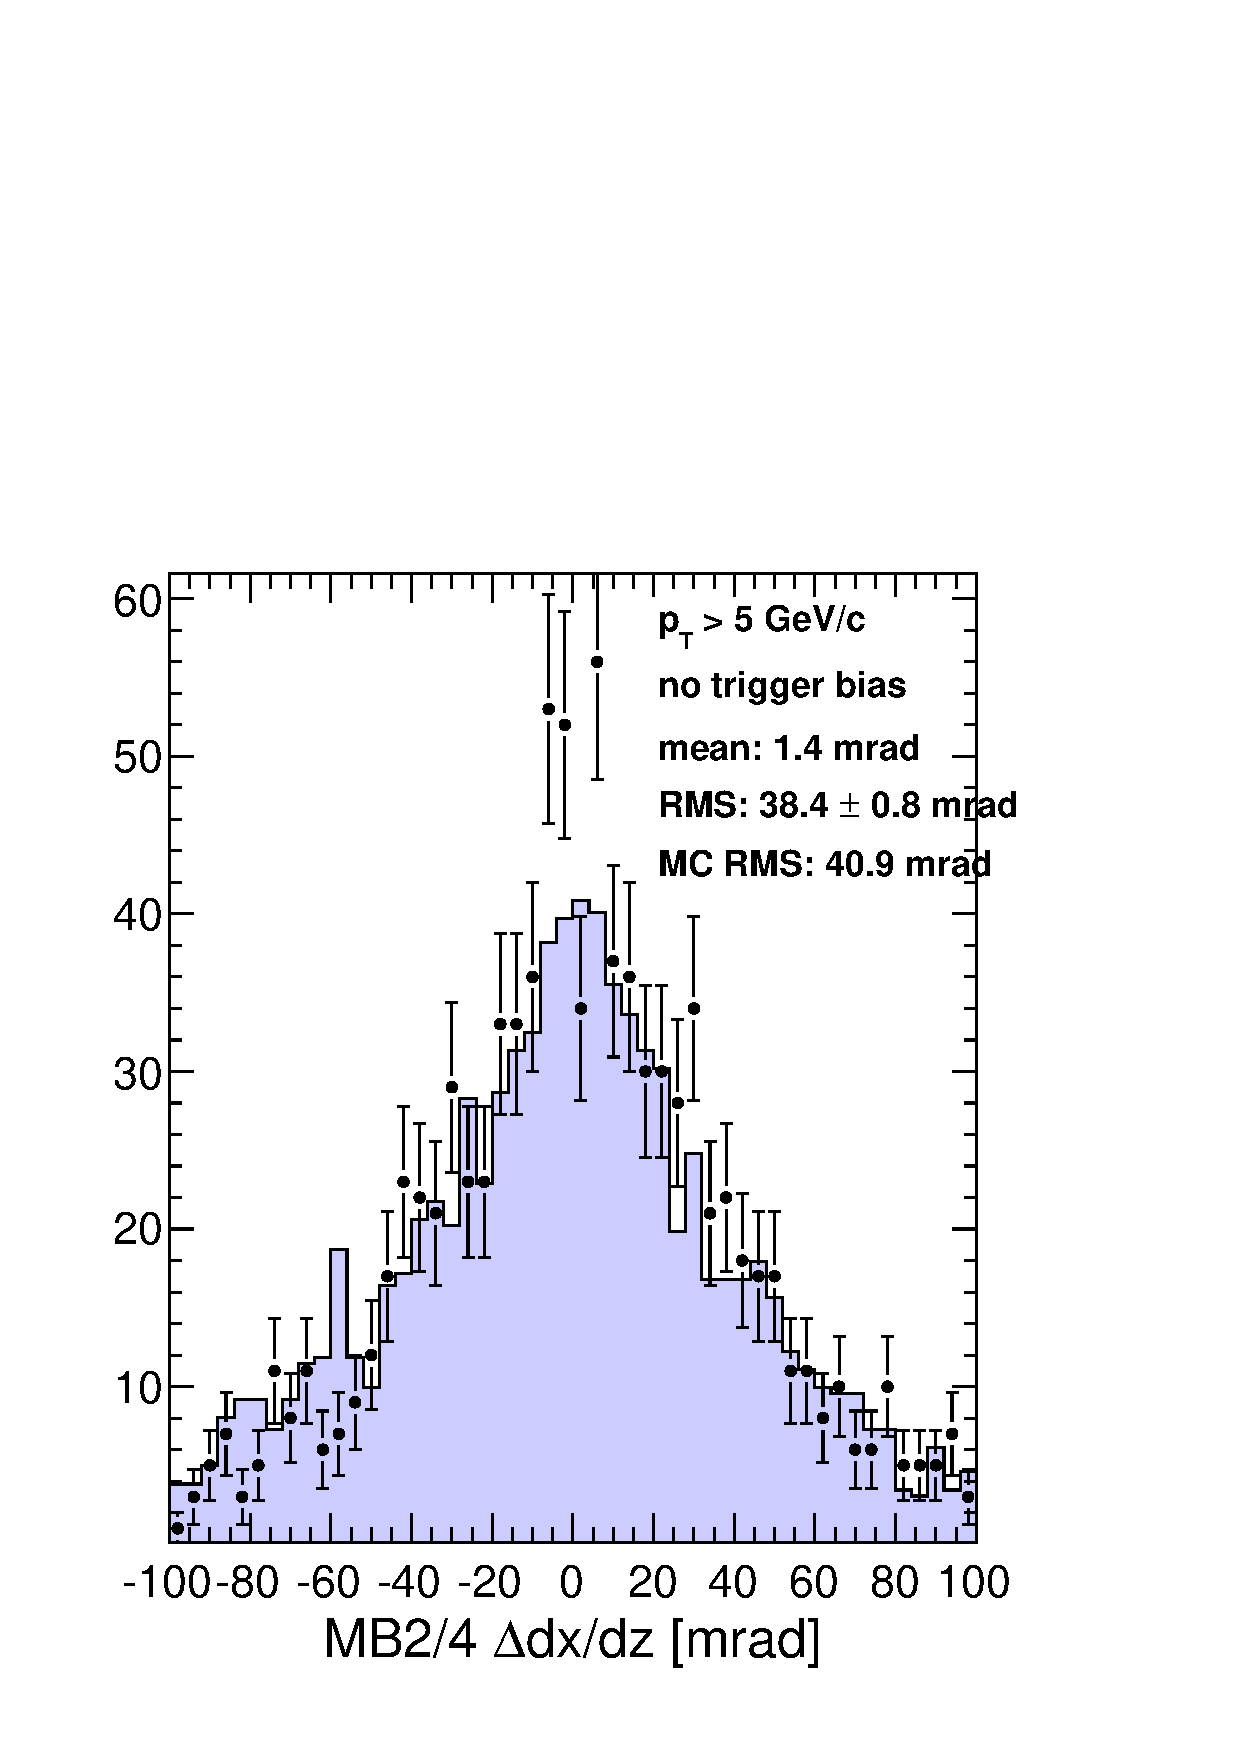
\includegraphics[width=0.24\linewidth]{mb24_dXdZ.pdf}
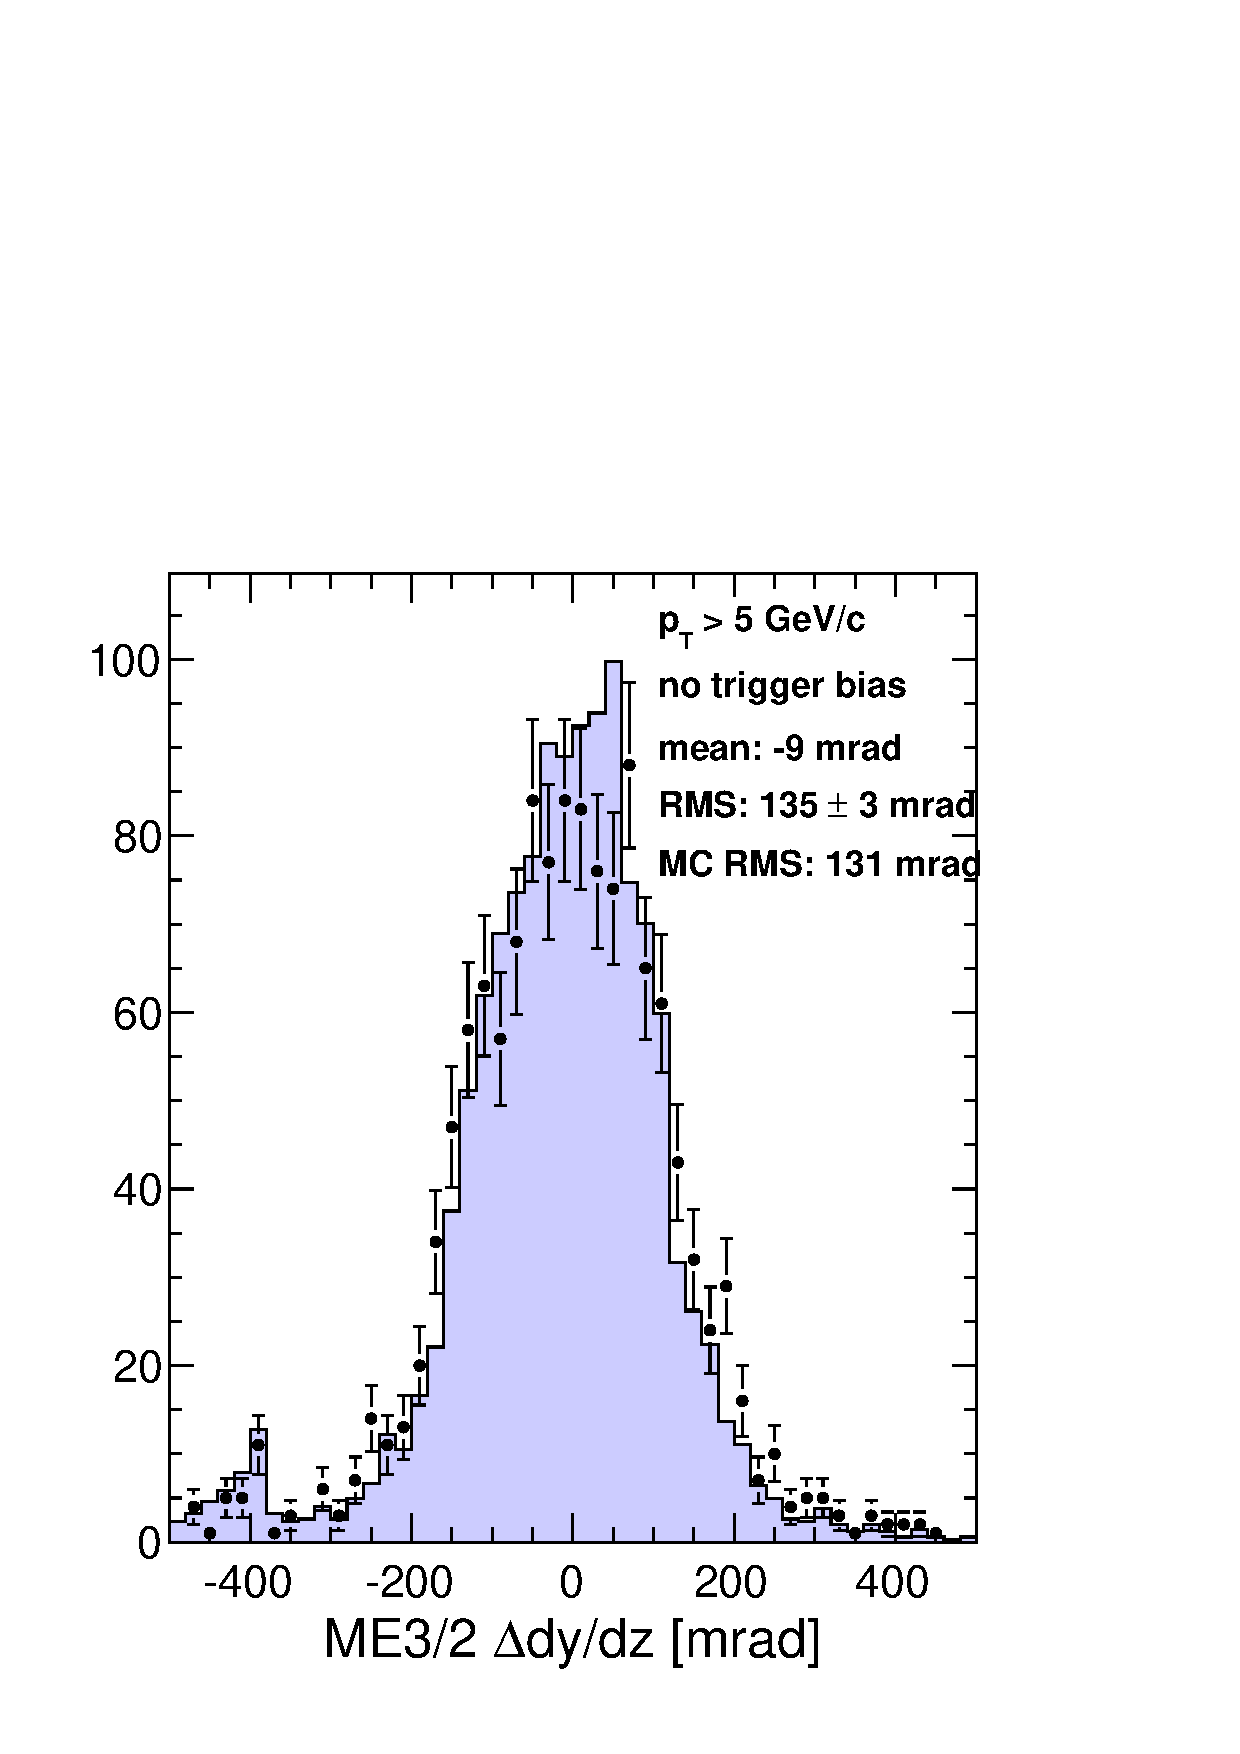
\includegraphics[width=0.24\linewidth]{me32_dYdZ.pdf}
\end{frame}

\begin{frame}
\frametitle{Dependence on detectors}

\begin{itemize}
\item MC is a little wider than the data everywhere
\item MC has STARTUP conditions re-tracked with IDEAL alignment: could
  be the influence of mis{\it calibrated} hits?
\end{itemize}
\begin{center}
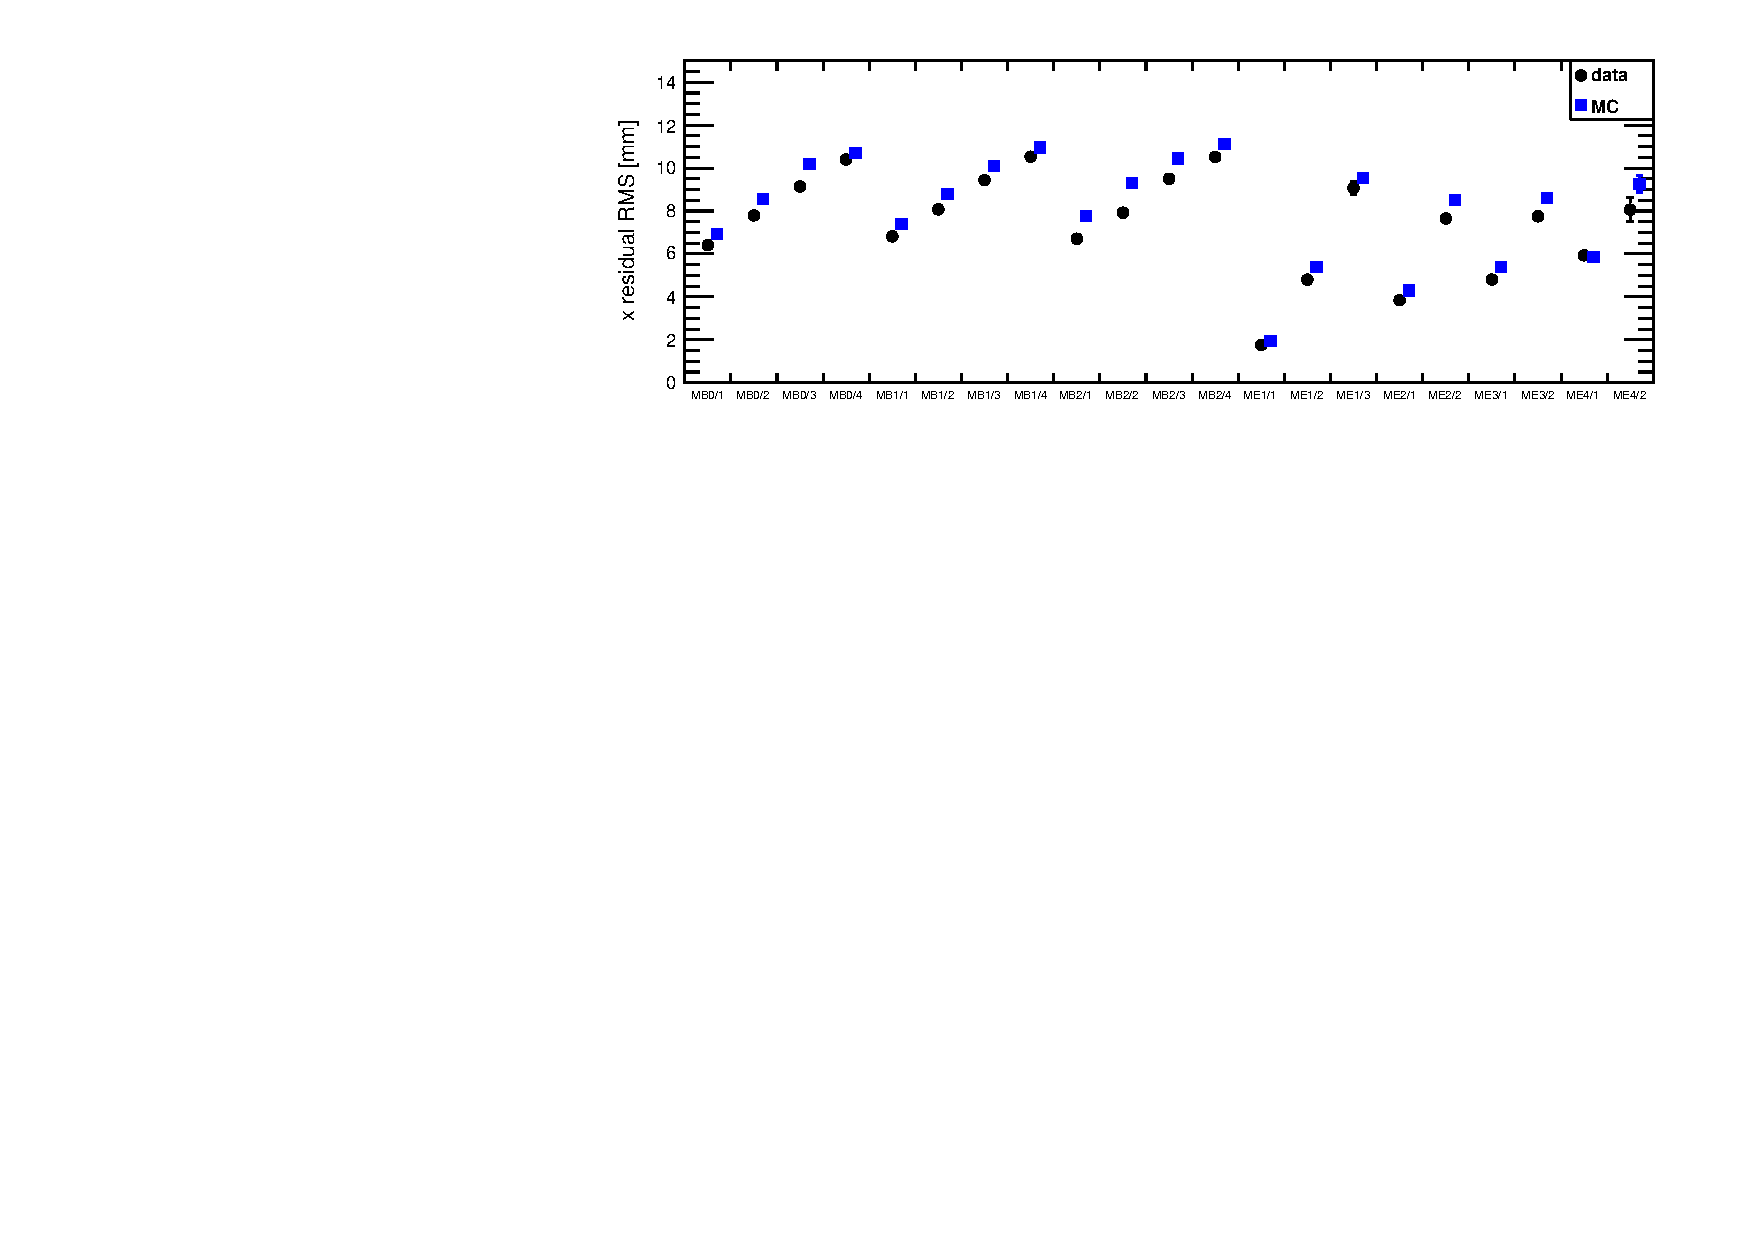
\includegraphics[width=0.9\linewidth]{summaryX.pdf}

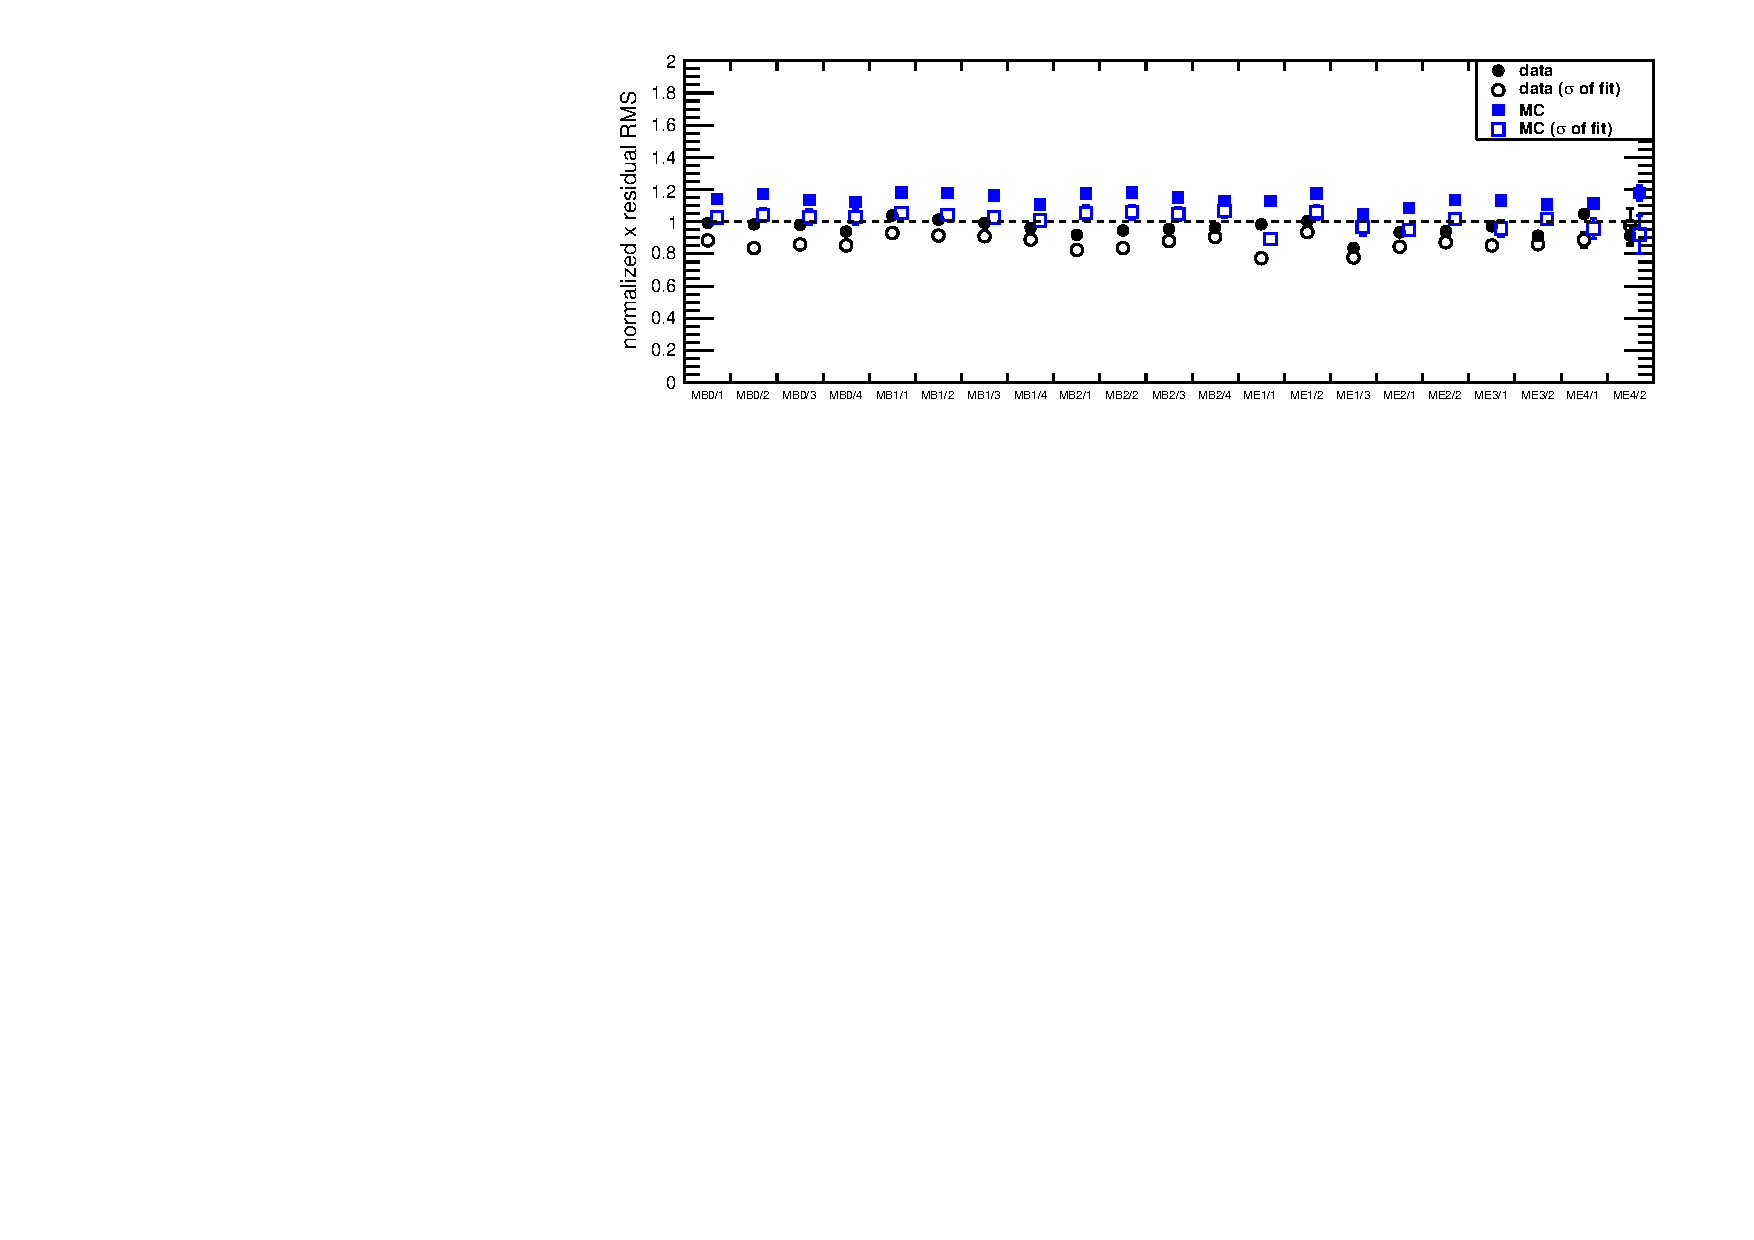
\includegraphics[width=0.9\linewidth]{summaryXnorm.pdf}
\end{center}
\end{frame}

\begin{frame}
\frametitle{Dependence on detectors}

\begin{itemize}
\item Same for $y$
\item Compared with standard RelVals (similar results):
\href{http://cmsdoc.cern.ch/cms/Physics/muon/CMSSW/Performance/RecoMuon/MuonIdentification/}{\textcolor{blue}{\tt \tiny http://cmsdoc.cern.ch/cms/Physics/muon/CMSSW/Performance/RecoMuon/MuonIdentification/}}
\end{itemize}
\begin{center}
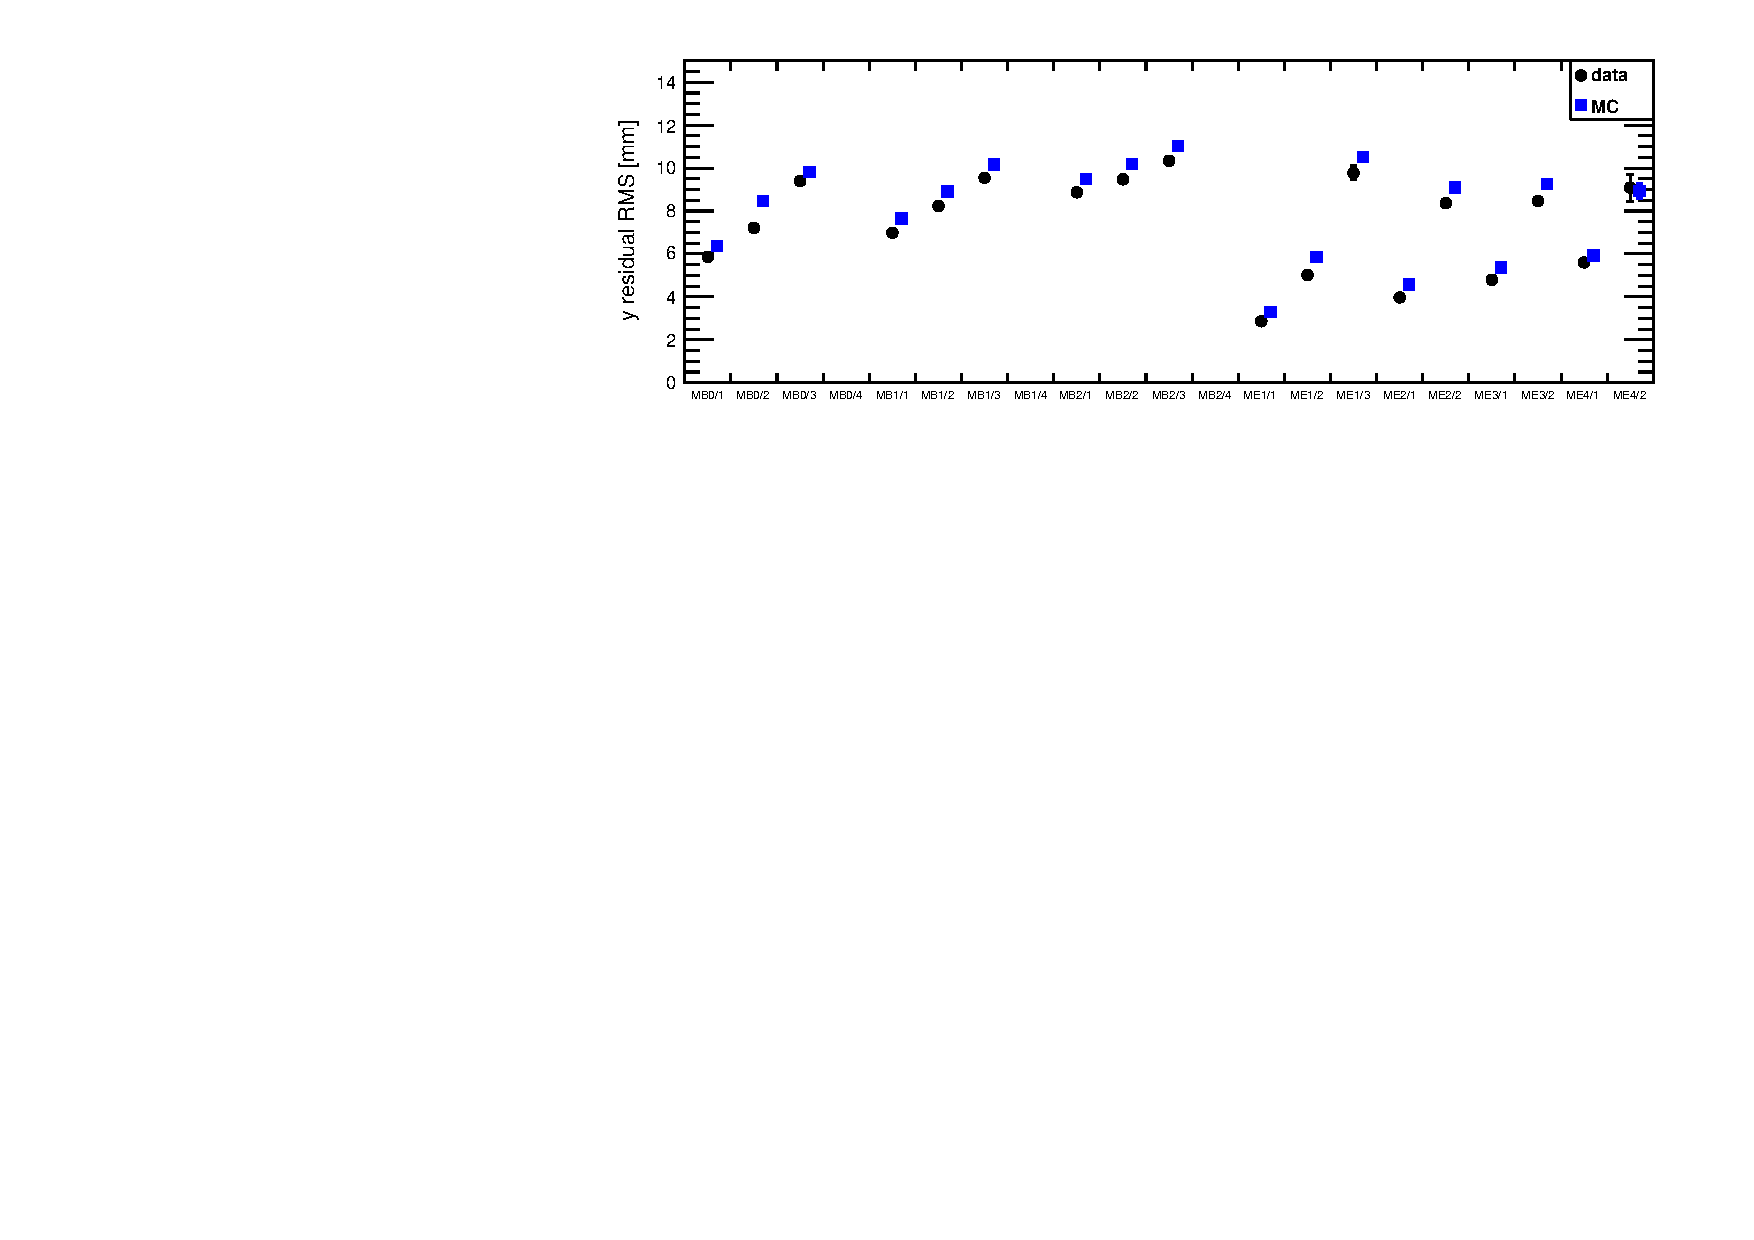
\includegraphics[width=0.9\linewidth]{summaryY.pdf}

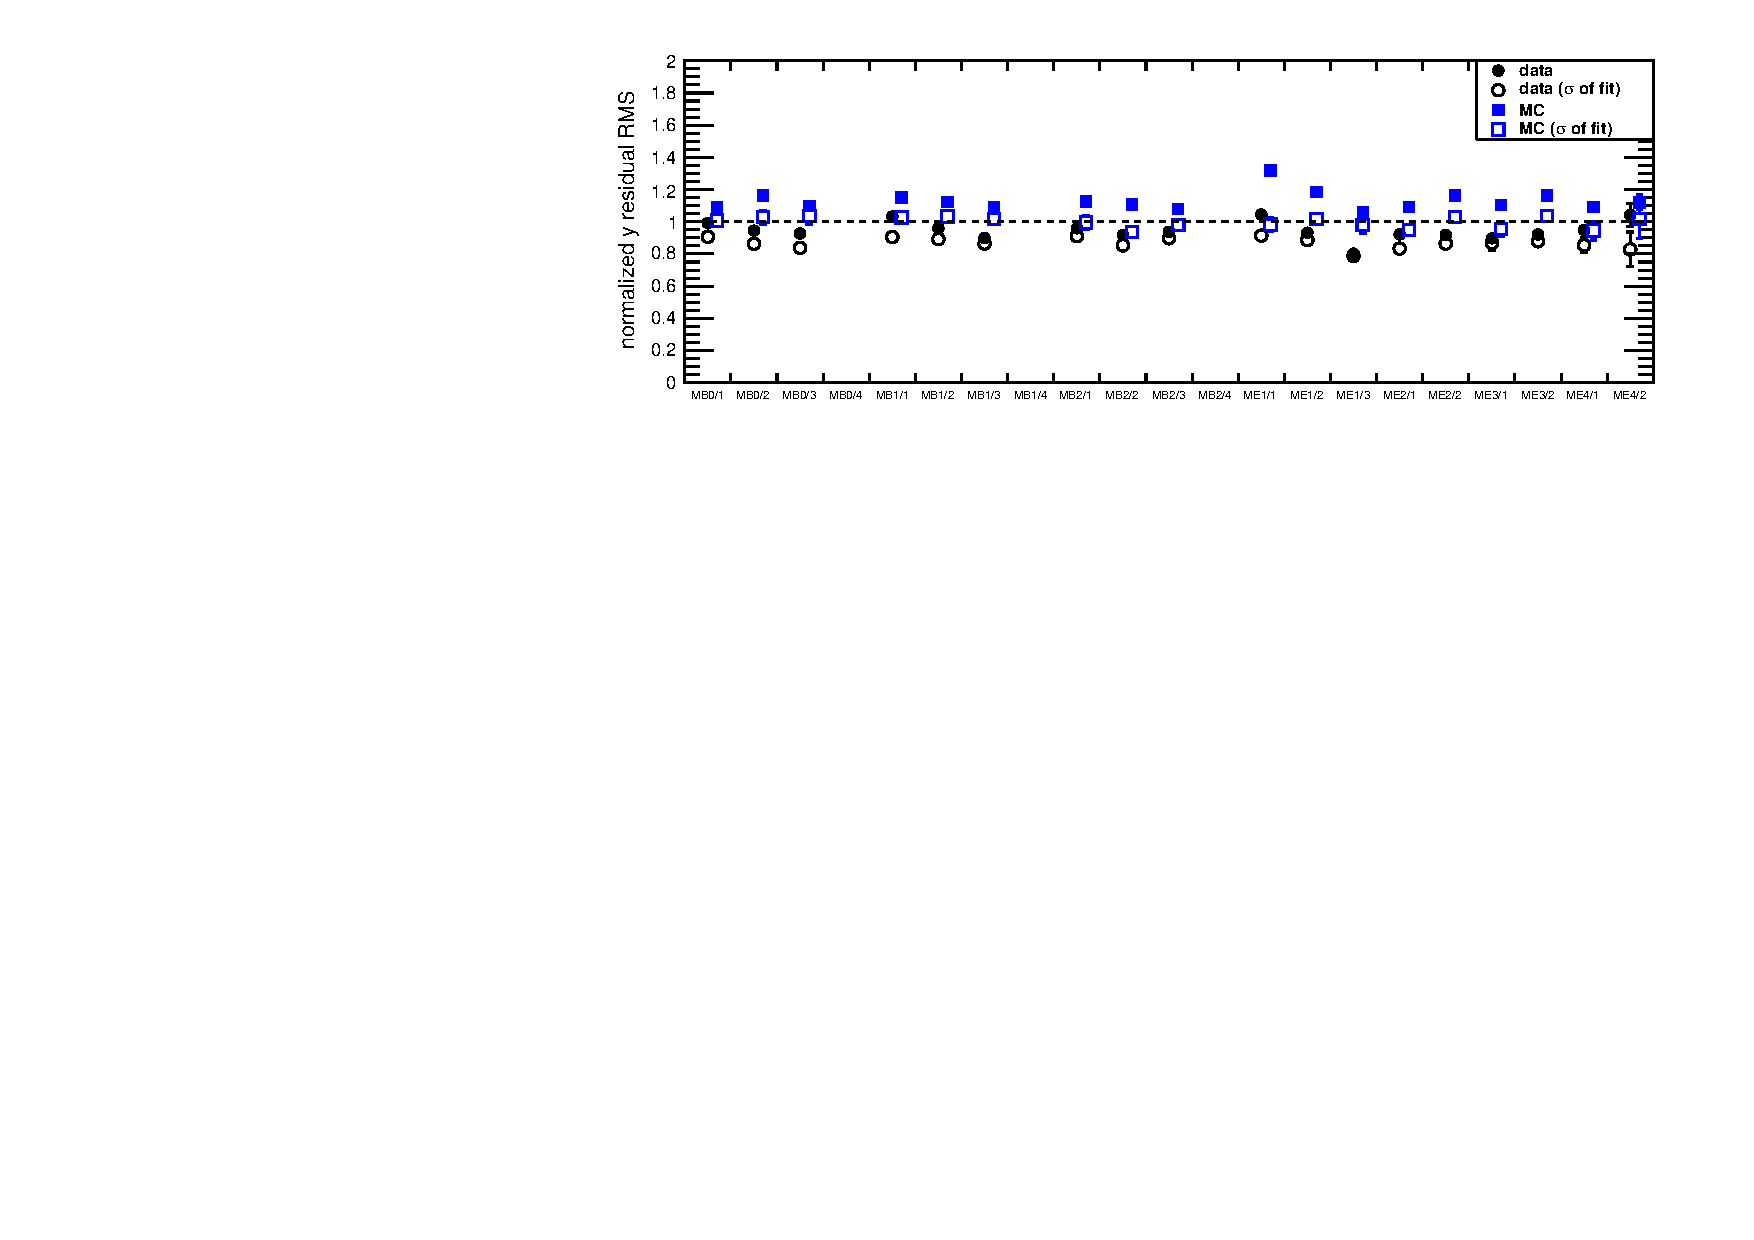
\includegraphics[width=0.9\linewidth]{summaryYnorm.pdf}
\end{center}
\end{frame}

\begin{frame}
\frametitle{Dependence on detectors}

\begin{itemize}
\item Endcap normalized dx/dz distributions have tails (RMS $>$ $\sigma$)
\item $dx/dz$ has not been aligned in the endcap
\item But this pattern is reproduced in MC--- doesn't seem like misalignment is the problem
\end{itemize}
\begin{columns}
\column{0.8\linewidth}
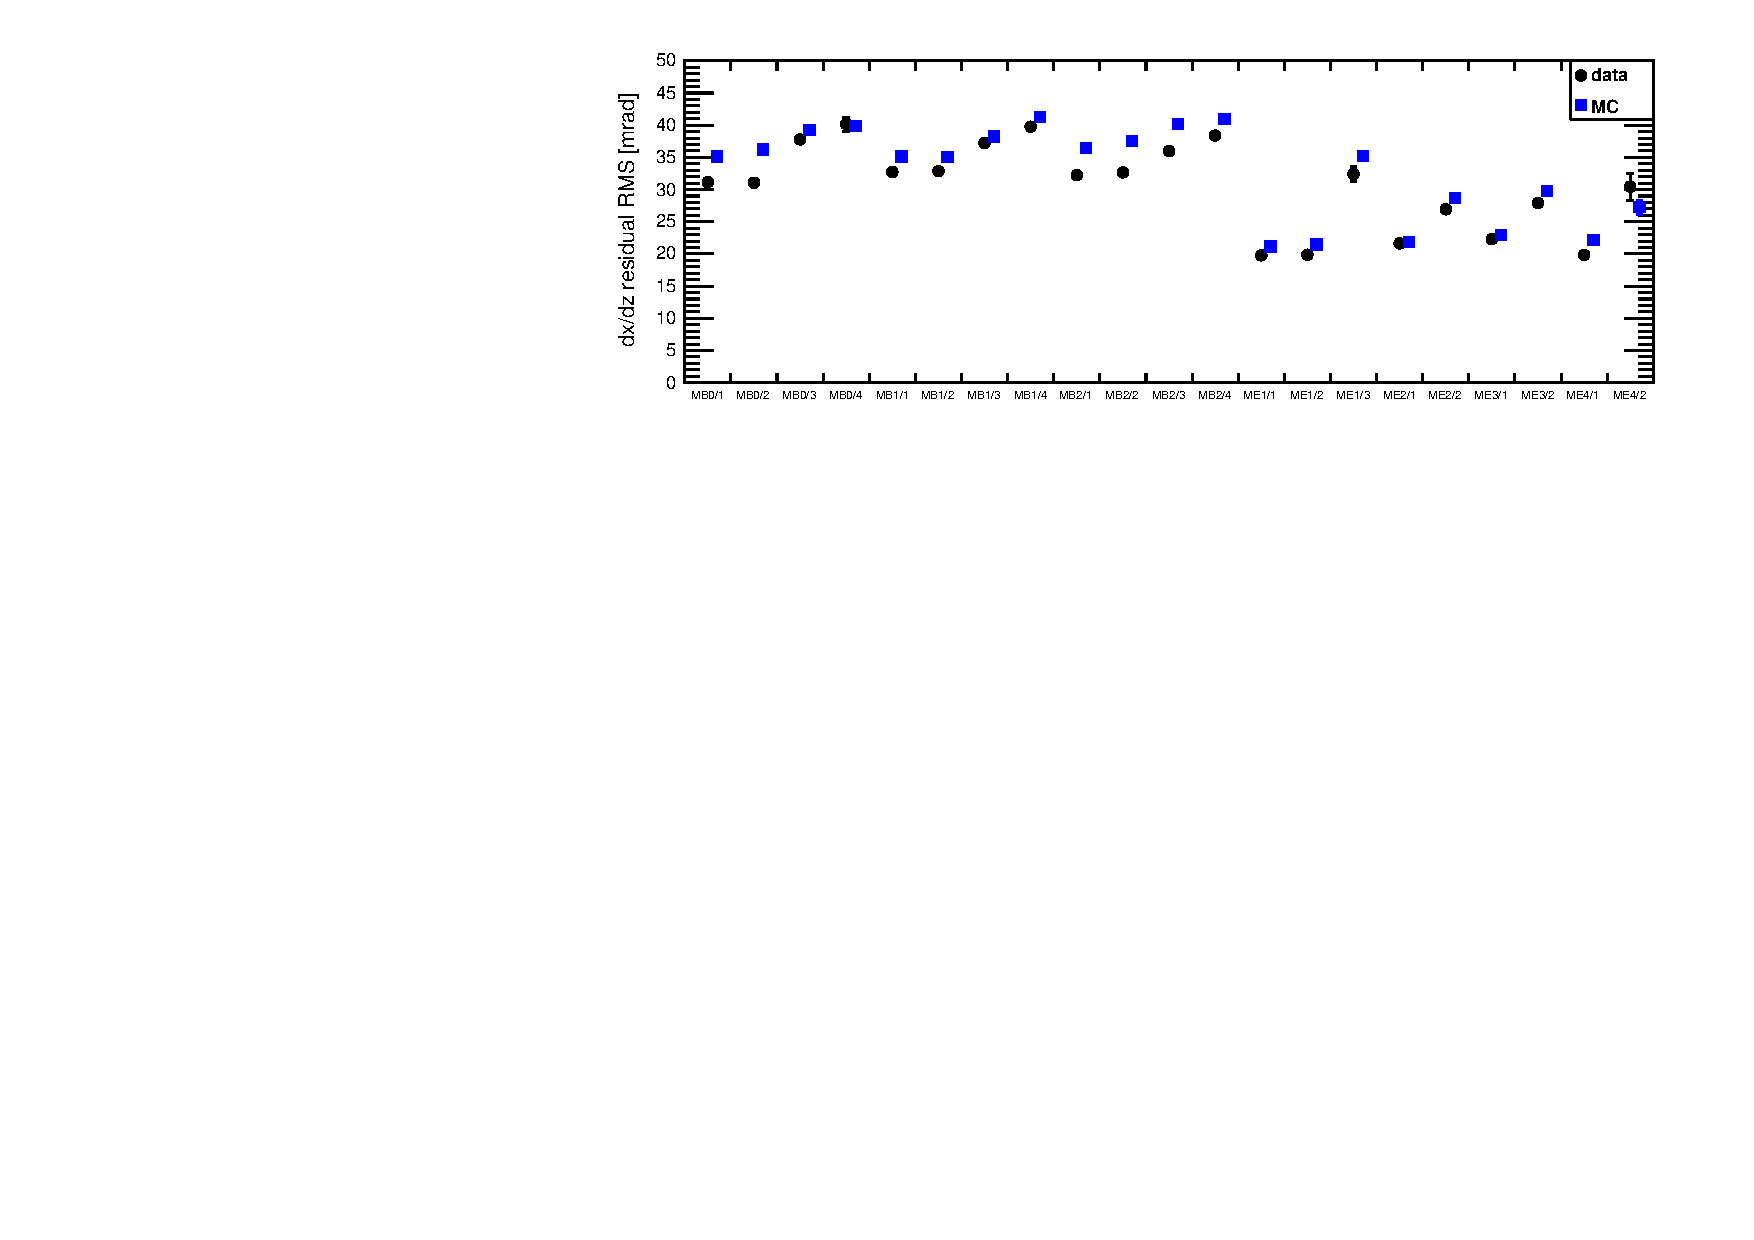
\includegraphics[width=\linewidth]{summarydXdZ.pdf}

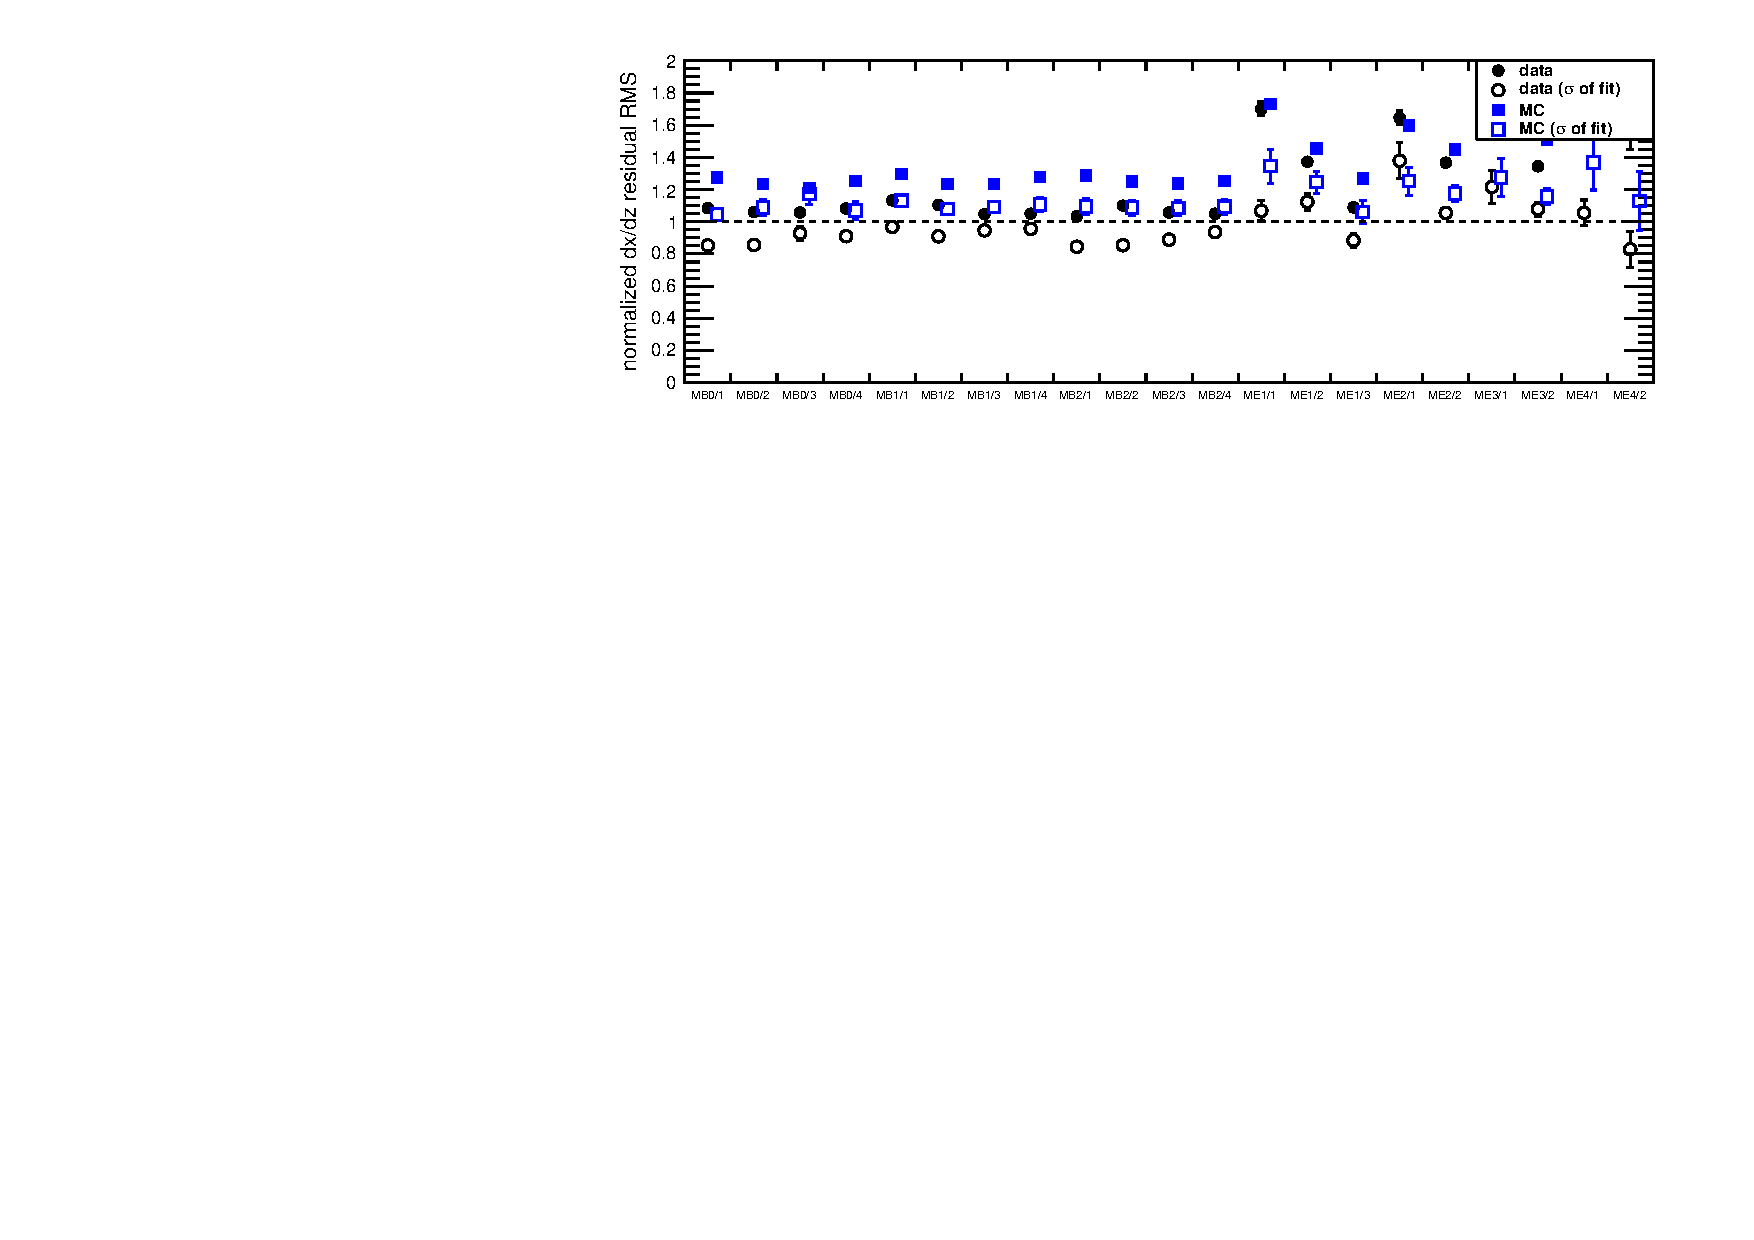
\includegraphics[width=\linewidth]{summarydXdZnorm.pdf}

\column{0.2\linewidth}
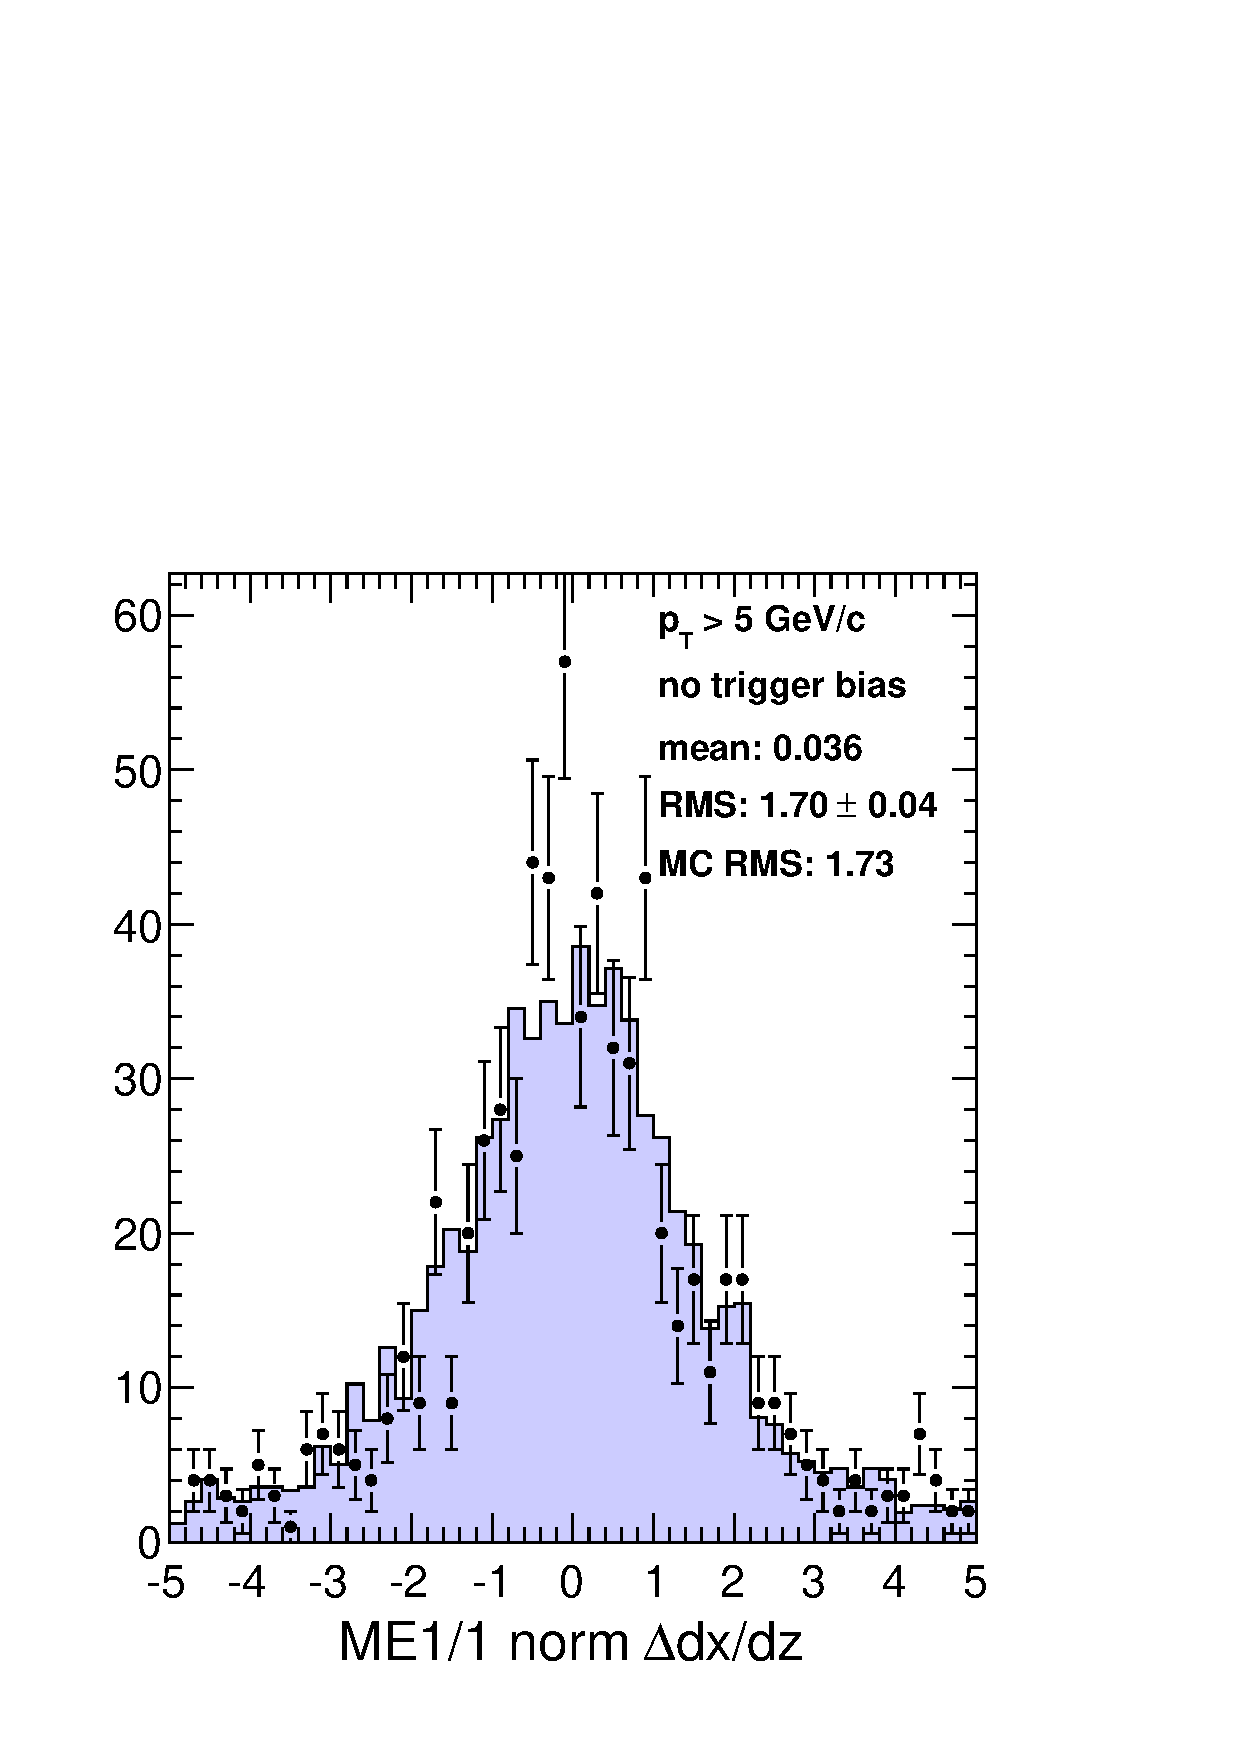
\includegraphics[width=\linewidth]{me11_dXdZnorm.pdf}

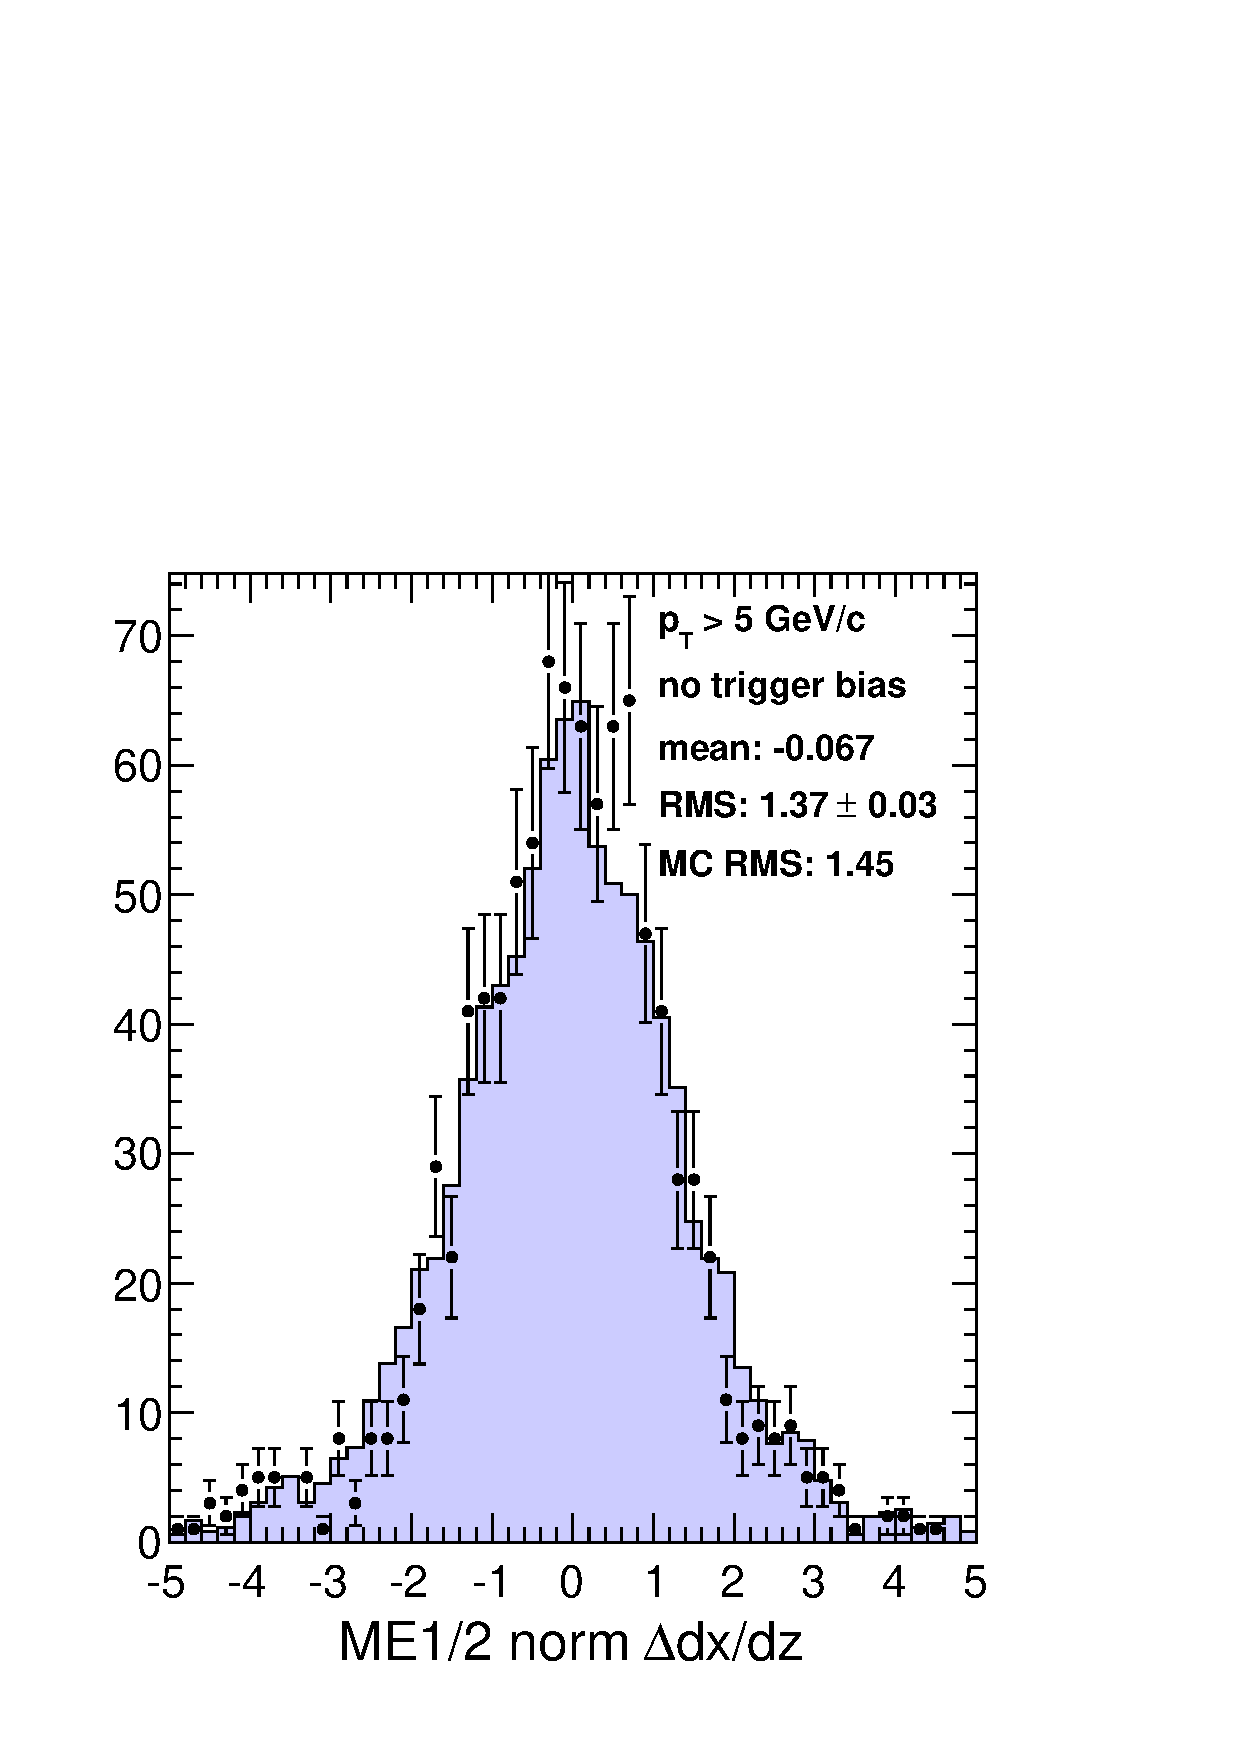
\includegraphics[width=\linewidth]{me12_dXdZnorm.pdf}
\end{columns}
\end{frame}

\begin{frame}
\frametitle{Dependence on detectors}

\begin{itemize}
\item The same can be said for $dy/dz$ in the barrel
\item Discrepancy in MB0/2 and MB0/3: MC has large tails\ldots?
\end{itemize}
\begin{columns}
\column{0.8\linewidth}
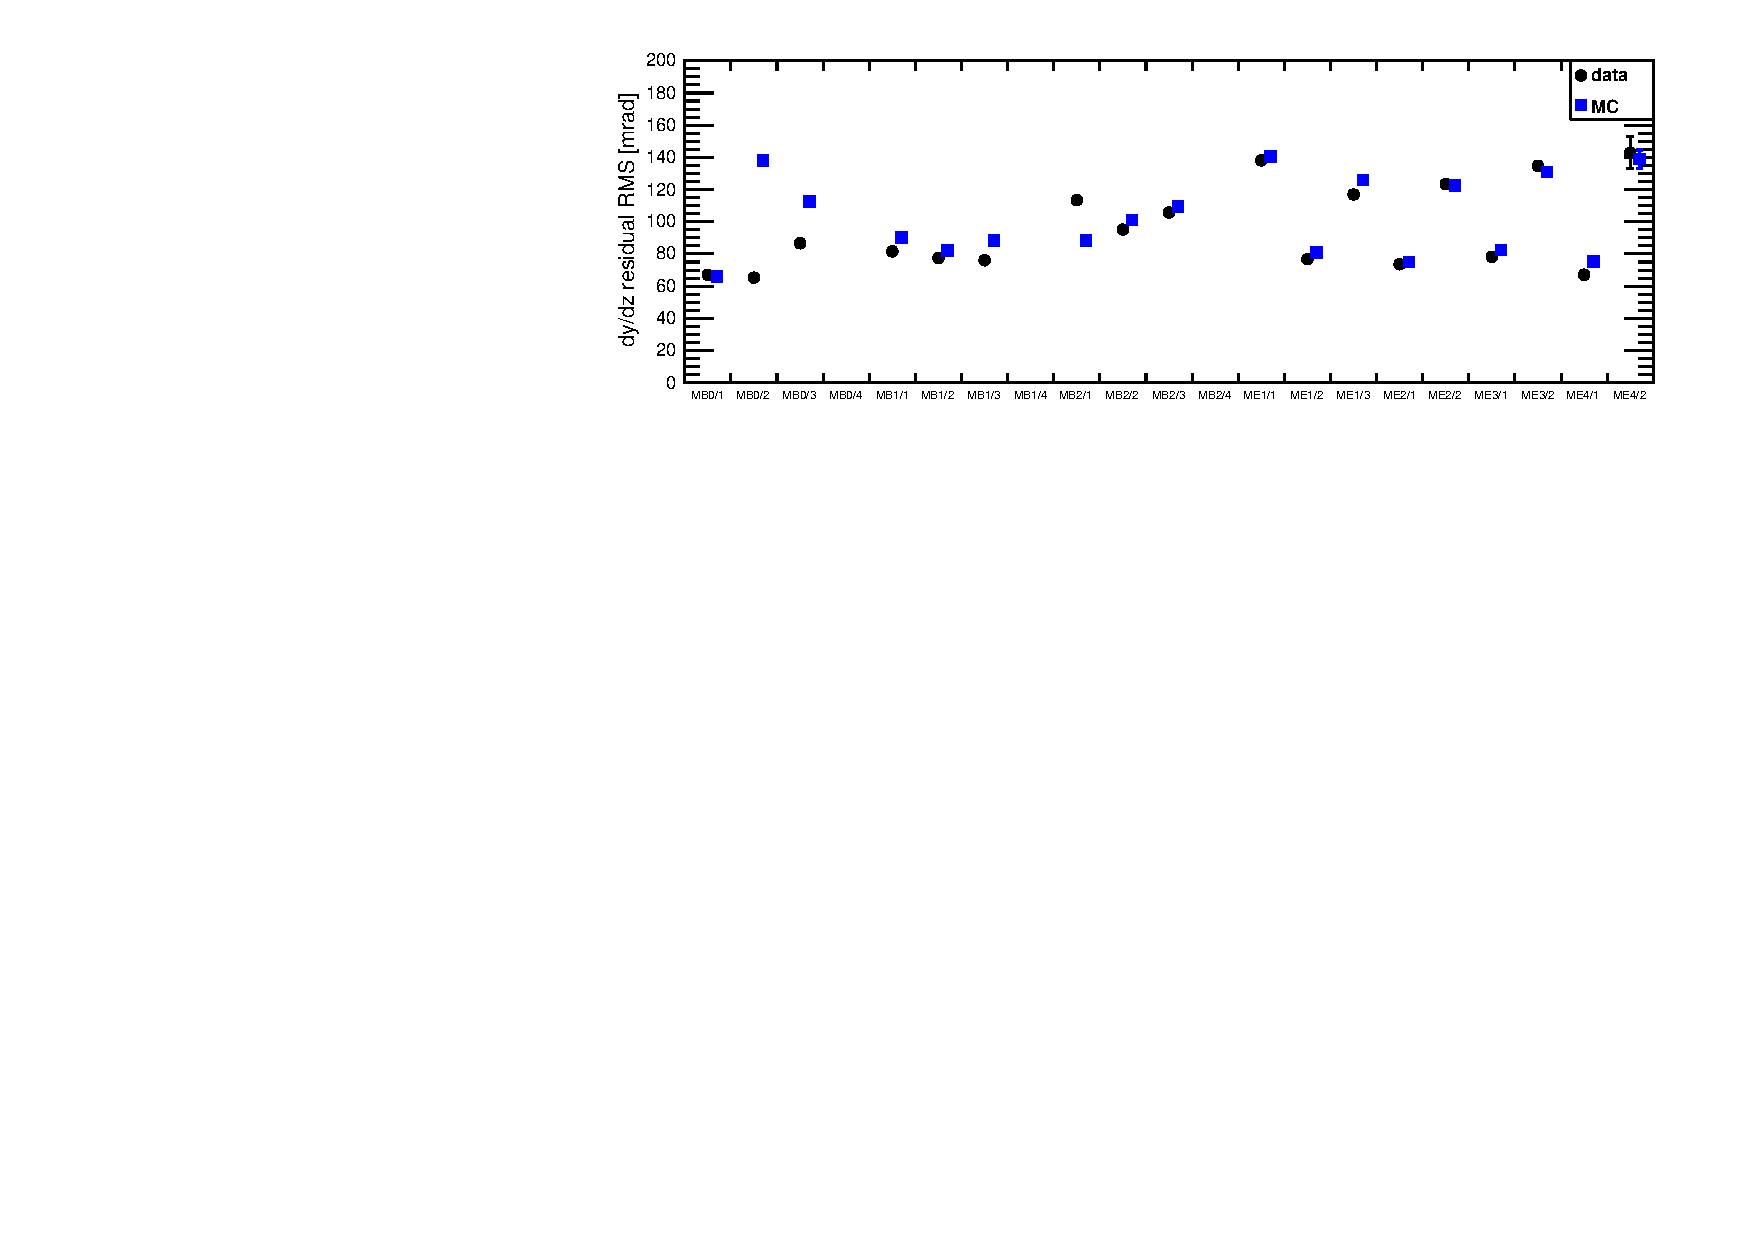
\includegraphics[width=\linewidth]{summarydYdZ.pdf}

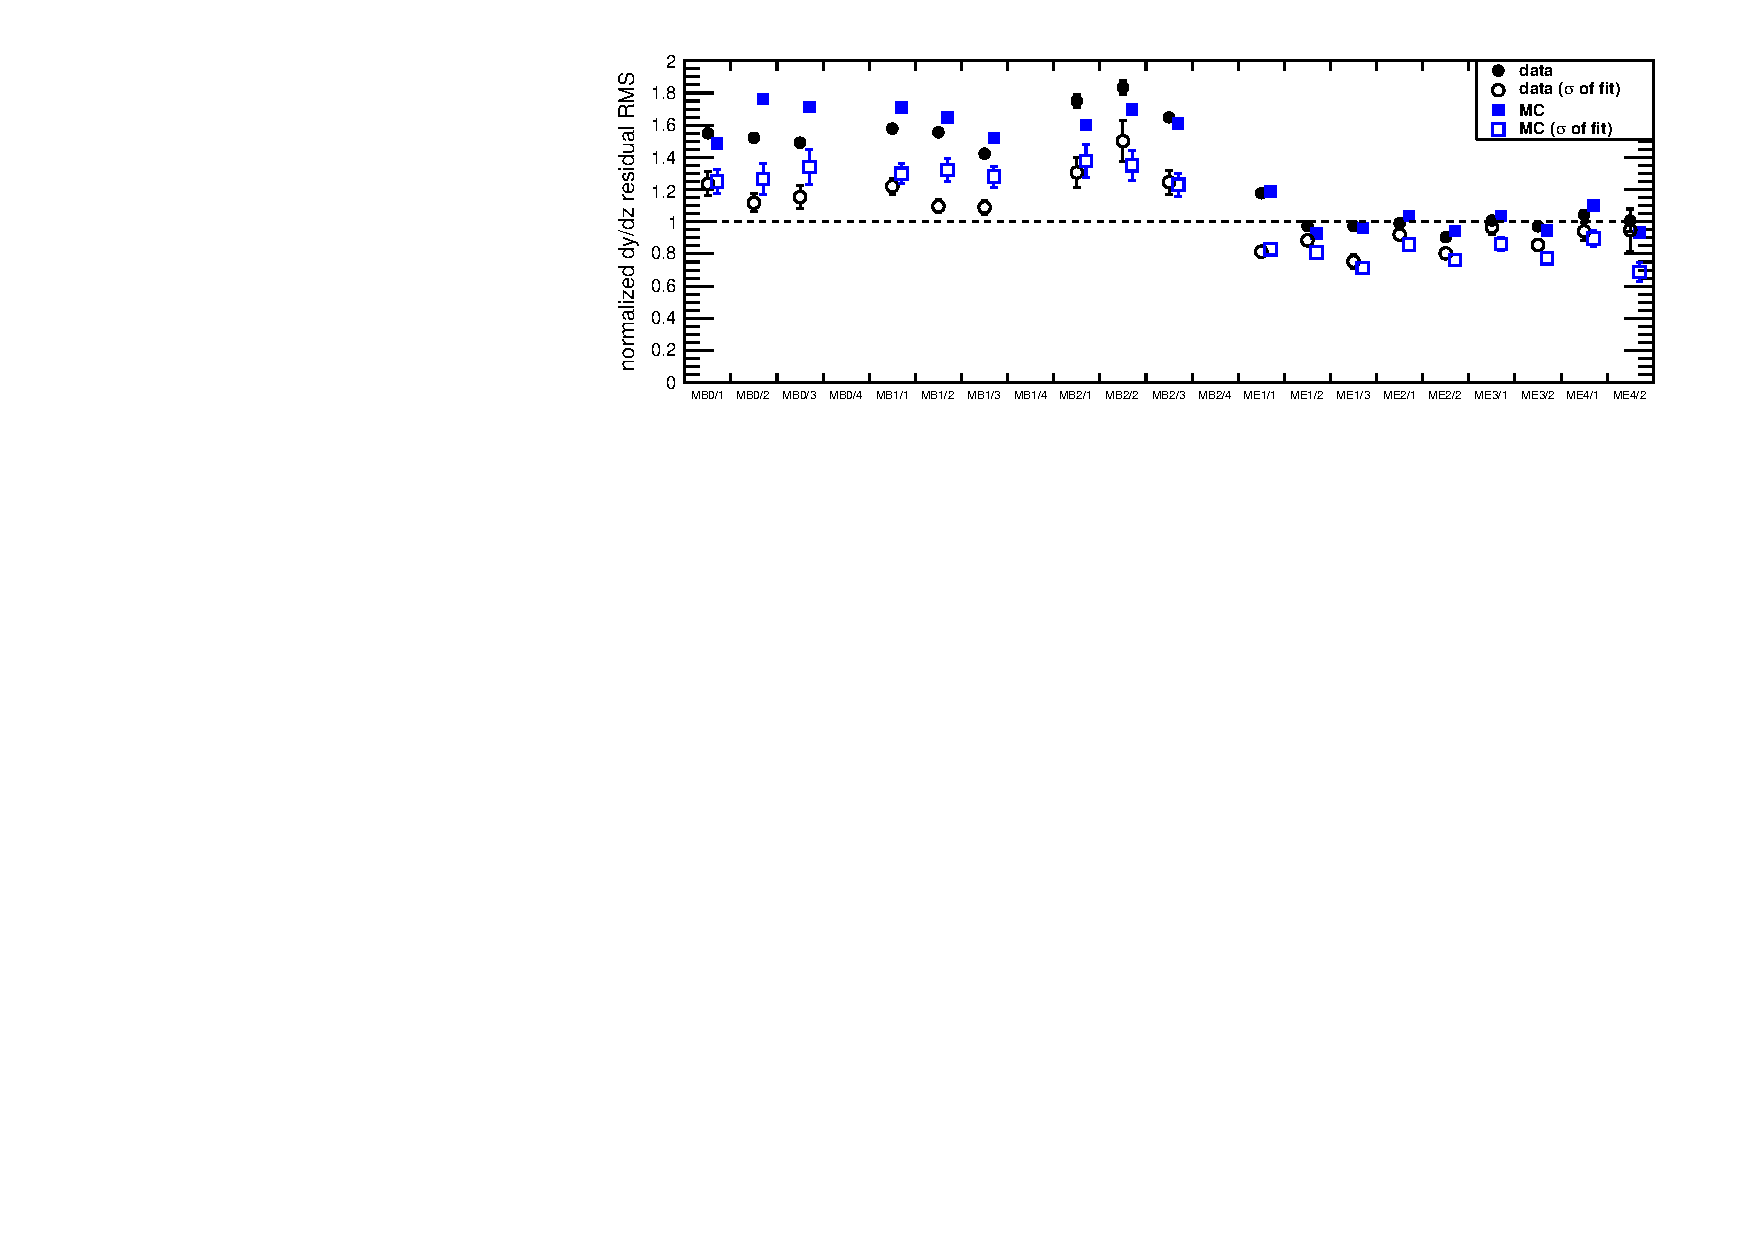
\includegraphics[width=\linewidth]{summarydYdZnorm.pdf}

\column{0.2\linewidth}

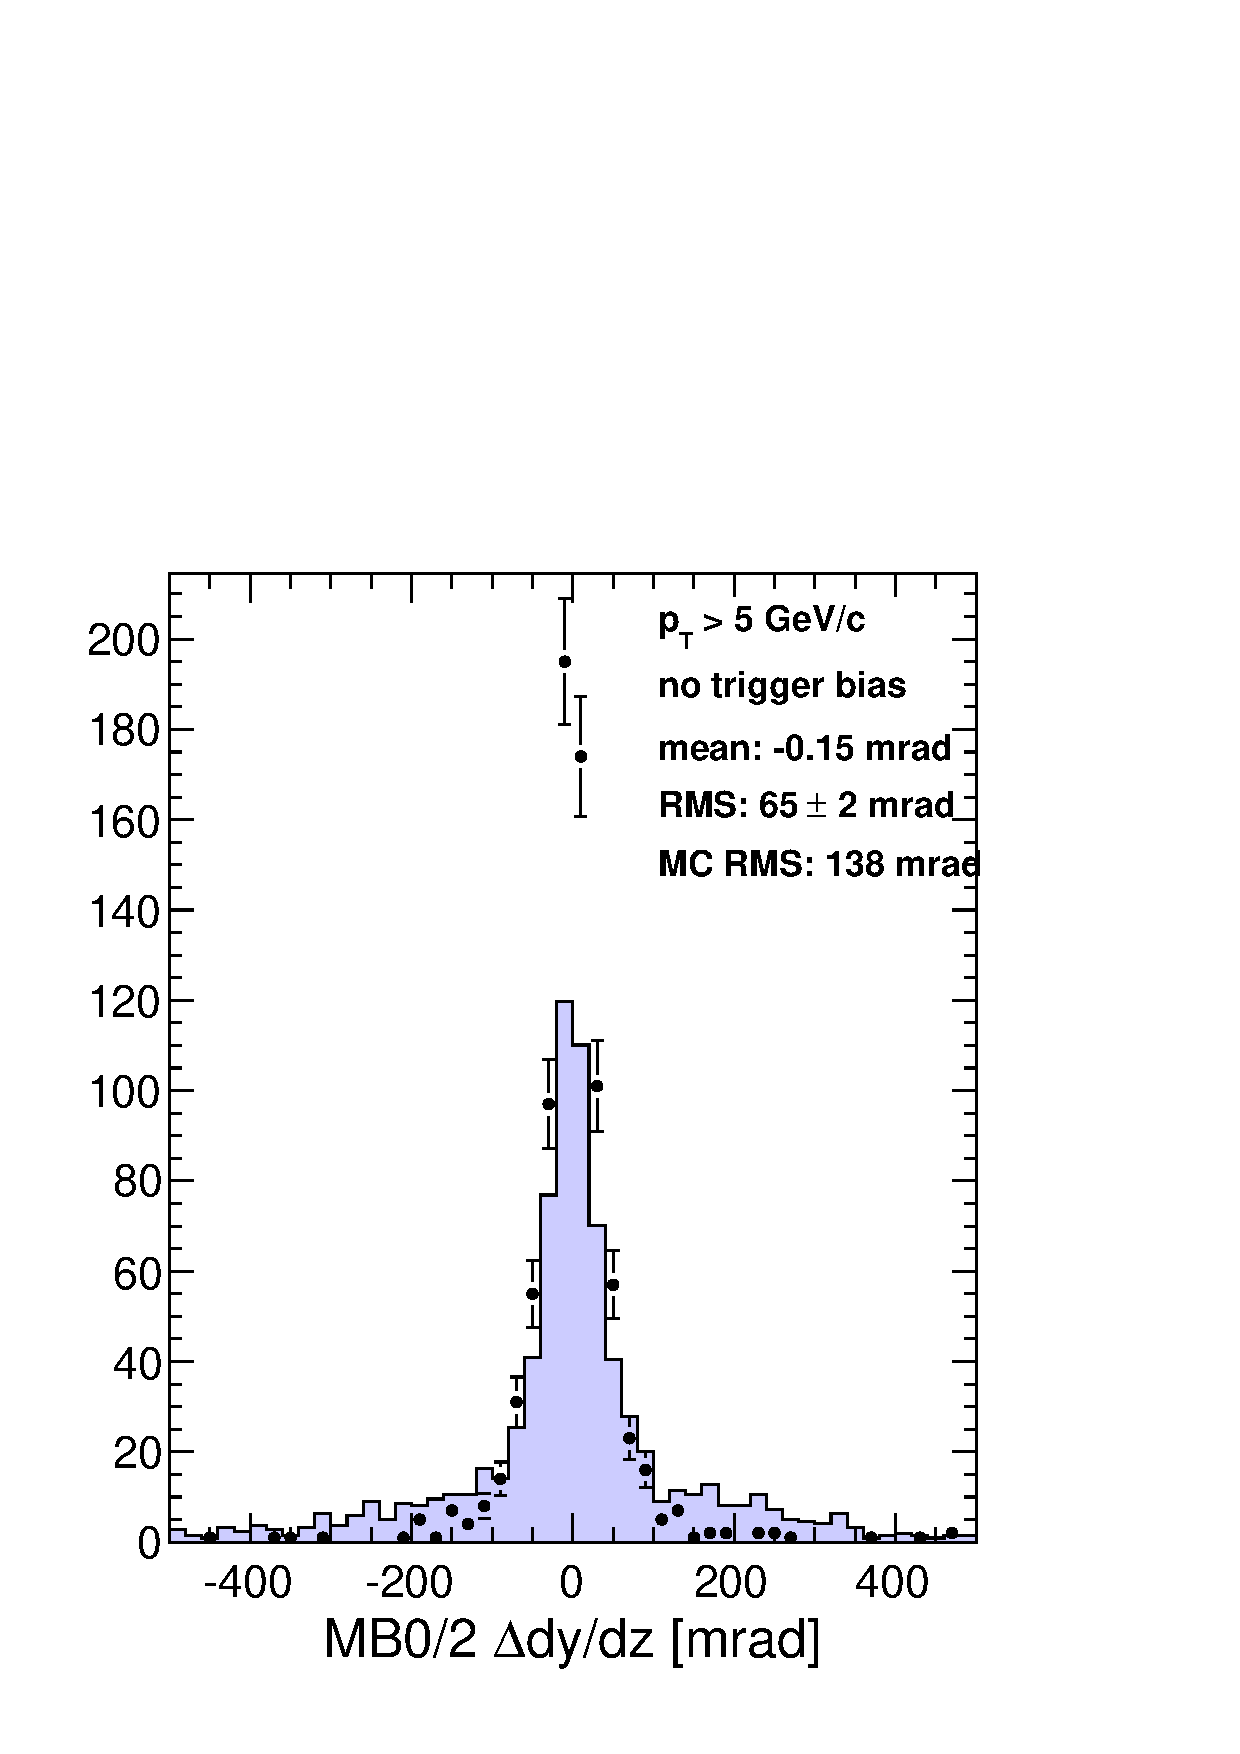
\includegraphics[width=\linewidth]{mb02_dYdZ.pdf}

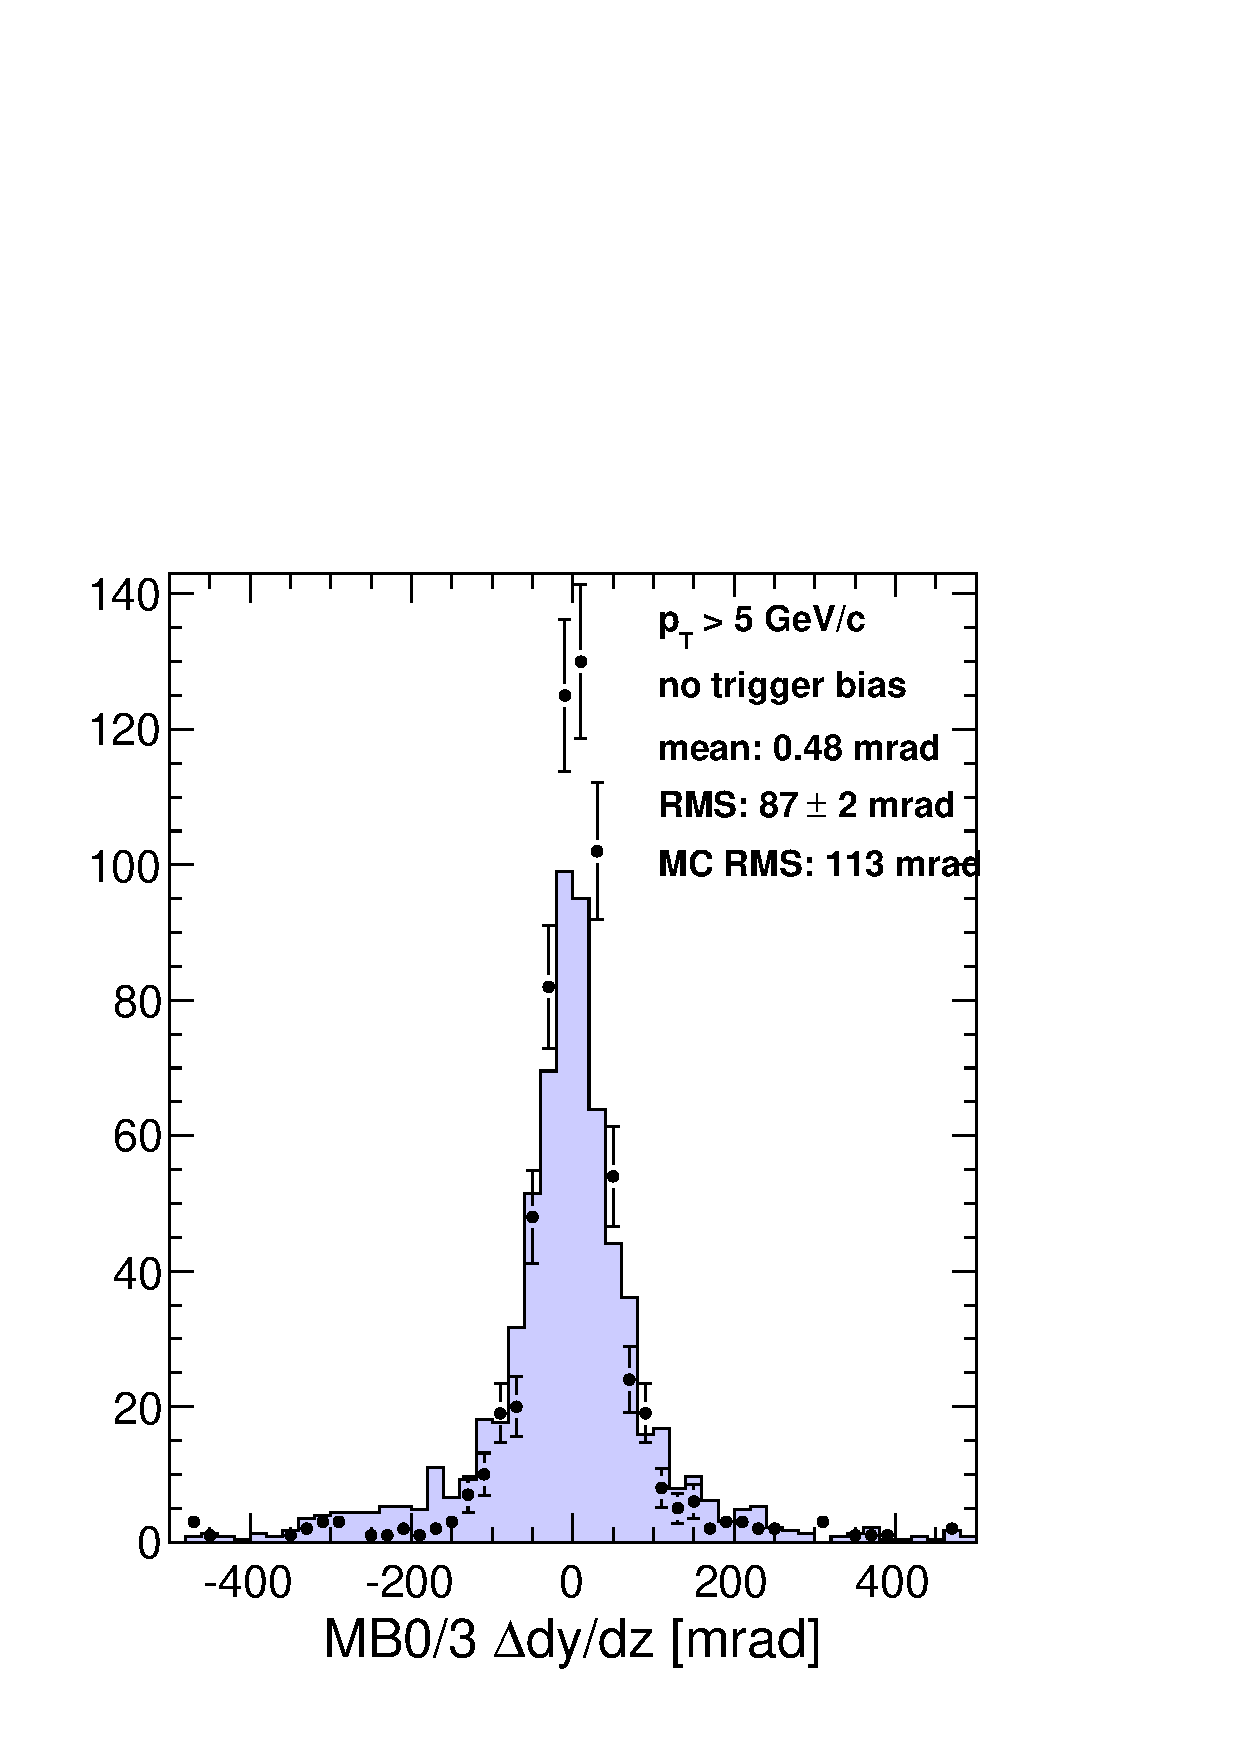
\includegraphics[width=\linewidth]{mb03_dYdZ.pdf}
\end{columns}
\end{frame}

\begin{frame}
\frametitle{Dependence on detectors}

\begin{itemize}
\item Oddity in endcap: discrete peaks in $dy/dz$ residuals, reproduced by Monte Carlo and observed in standard RelVal plots (right)
\item Could be related to granularity of CSC wire-groups?
\end{itemize}

\vfill
\begin{center}
\mbox{ } \hfill 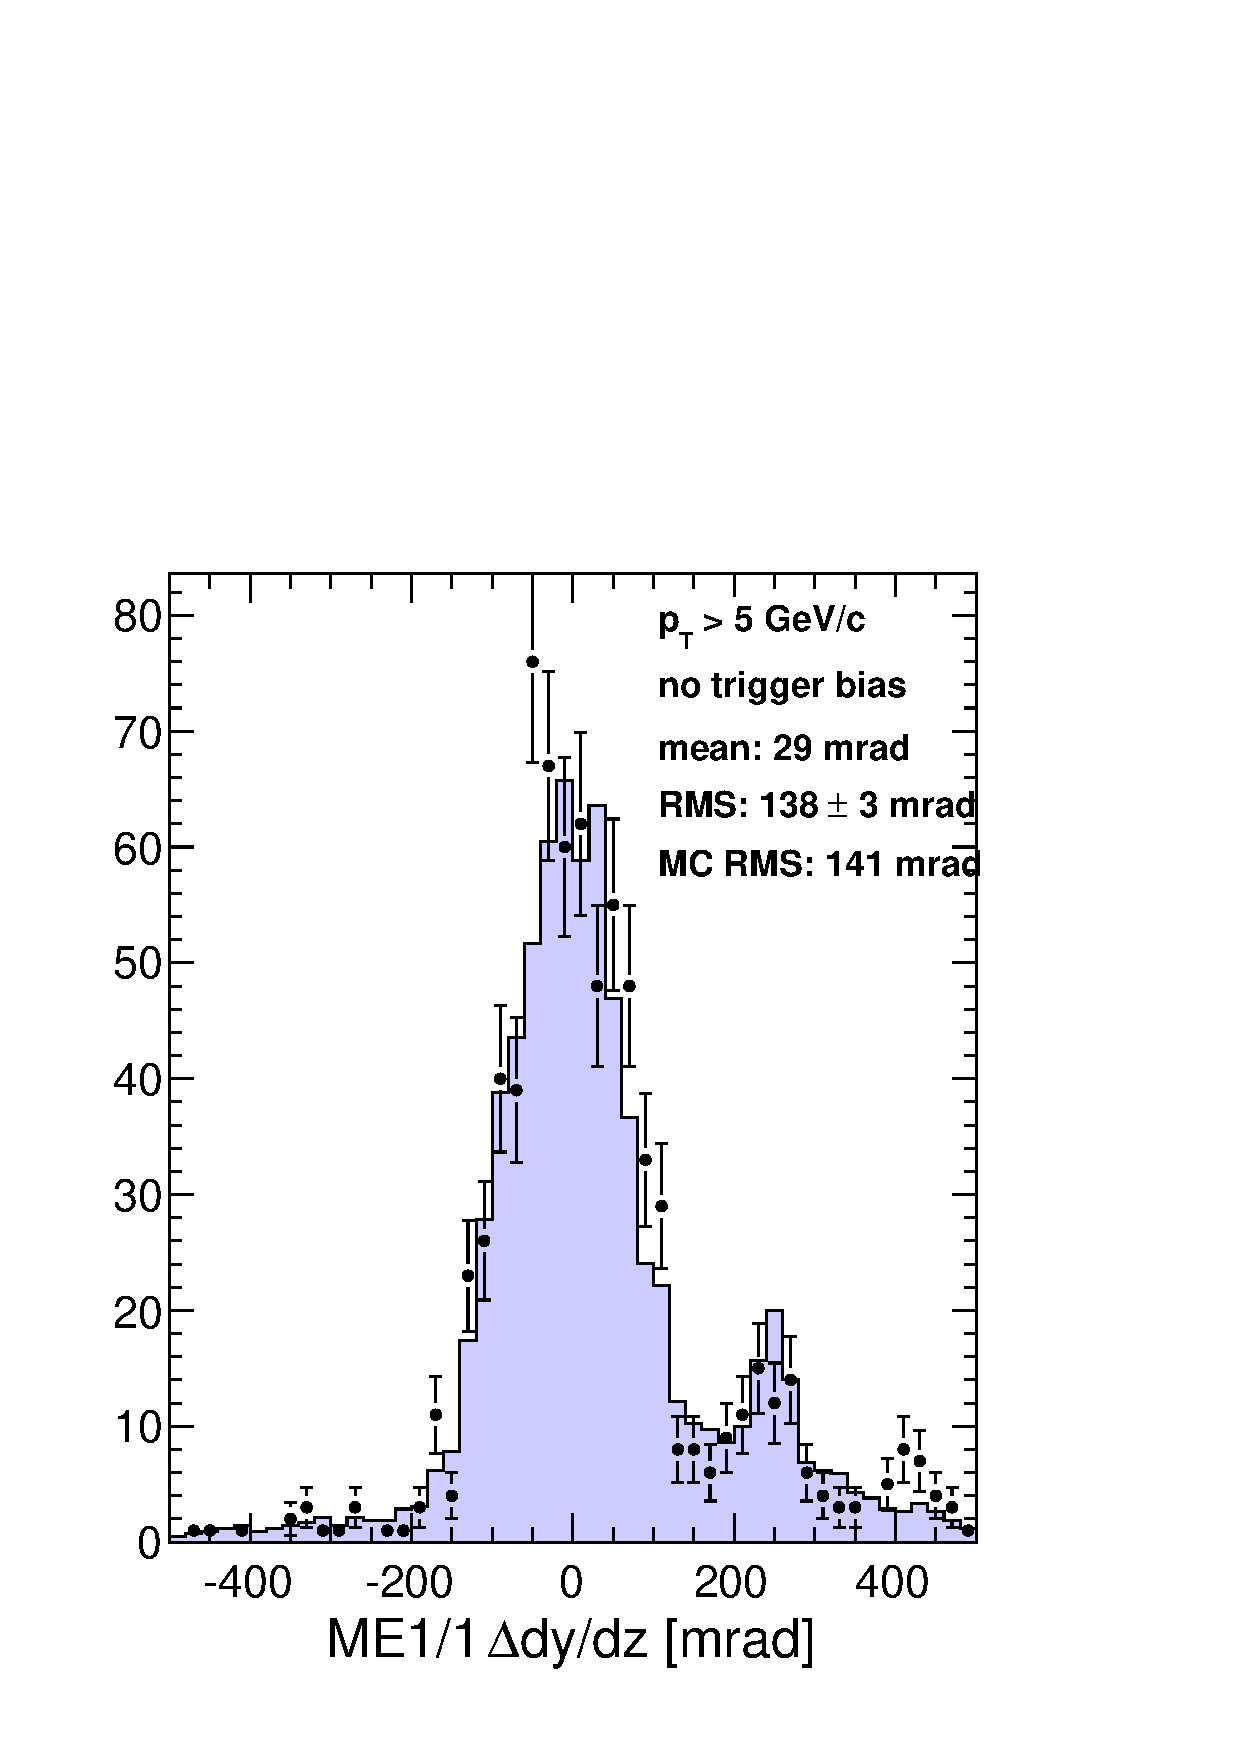
\includegraphics[height=3.2 cm]{me11_dYdZ.pdf} \hfill 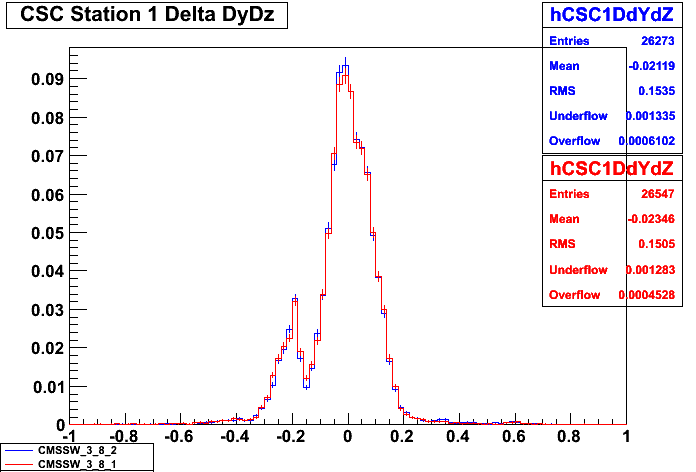
\includegraphics[height=3.2 cm]{me11_dydz_relvals.png} \hfill \mbox{ }
\end{center}
\end{frame}

\begin{frame}
\frametitle{Next steps}
\begin{itemize}
\item Data/MC comparisons
\begin{enumerate}\setlength{\itemsep}{0.2 cm}
\item \sout{check residuals distributions with these track/event cuts}
\item modifications to residuals distributions when two muons cross (pair-gun MC; enough statistics to check data, too?)
\item compare kinematic quantities (momenta, angular distributions)
\item find all missing background samples (particularly the mysterious low-mass contribution)
\end{enumerate}
\item Trigger efficiency study
\begin{enumerate}
\item reconstructing one $p_T > 11$~GeV/$c$, $|\eta| < 2.1$
  StandAloneMuon in the presence of nearby/overlapping muons
\item HLT and L1 efficiencies, given the above
\end{enumerate}
\item Estimating backgrounds from data
\item Efficiency from tag-and-probe of boosted $J/\psi$?
\end{itemize}
\end{frame}


\begin{frame}
\frametitle{Conclusions}
\begin{itemize}
\item Basically good data/MC agreement out-of-the-box
\item Discrepancies:
\begin{itemize}\setlength{\itemsep}{0.1 cm}
\item missing prompt $J/\psi$, $\psi'$ (not a problem; just add them)
\item underproduced $\phi(1020)$ and missing $\omega(782)$ {\scriptsize (possibly produce prompt samples by following example of prompt $J/\psi$? is it necessary?  only at few-percent level\ldots)}
\item excess of $m_\s{inv} < 0.3$~GeV/$c^2$ events: {\it needs to be understood}
\item residual vs.\ momentum bias in data and not Monte Carlo
\item residuals distributions are generally narrower in data
\end{itemize}

\item Discrepancies in residuals are not large enough to make much
  difference in cut efficiencies, since cuts are wide
\begin{itemize}
\item if efficiencies are taken from $J/\psi$ tag-and-probe in the
  future, it won't matter at all
\end{itemize}

\item Residuals information will be useful for muon alignment studies,
  but for this analysis, I can move on to higher-level distributions
\end{itemize}

\label{numpages}
\end{frame}

\end{document}
